\documentclass[a4paper, 10pt]{article}
\usepackage[margin=1in]{geometry}
\usepackage{amsfonts, amsmath, amssymb, amsthm}
%\usepackage[none]{hyphenat}
\usepackage[utf8]{inputenc}
\usepackage[english, main=ukrainian]{babel}
\usepackage{pgfplots}
\usepgfplotslibrary{fillbetween}
\usepackage{bm}
\usepackage{physics}
\usepackage[unicode]{hyperref}
\usepackage{scalerel,stackengine}
\usepackage{multicol}
\usepackage{tikz-cd}
\usetikzlibrary{fit,matrix}
\usepackage{enumitem}
\usepackage{graphicx}
\usepackage{centernot}


\usepackage{pdfpages}
\usepackage{caption}
\usepackage{float}
\usepackage{bbm}
\usepackage{physics}
\usetikzlibrary{spy}

\def\rightproof{$\boxed{\Rightarrow}$ }

\def\leftproof{$\boxed{\Leftarrow}$ }

\newtheoremstyle{theoremdd}% name of the style to be used
  {\topsep}% measure of space to leave above the theorem. E.g.: 3pt
  {\topsep}% measure of space to leave below the theorem. E.g.: 3pt
  {\normalfont}% name of font to use in the body of the theorem
  {0pt}% measure of space to indent
  {\bfseries}% name of head font
  {}% punctuation between head and body
  { }% space after theorem head; " " = normal interword space
  {\thmname{#1}\thmnumber{ #2}\textnormal{\thmnote{ \textbf{#3}\\}}}

\theoremstyle{theoremdd}
\newtheorem{theorem}{Theorem}[subsection]
\newtheorem{definition}[theorem]{Definition}
\newtheorem{example}[theorem]{Example}
\newtheorem{proposition}[theorem]{Proposition}
\newtheorem{remark}[theorem]{Remark}
\newtheorem{lemma}[theorem]{Lemma}
\newtheorem{corollary}[theorem]{Corollary}
\newtheorem*{definition*}{Definition.}
\newtheorem*{proposition*}{Proposition.}
\newtheorem*{remark*}{Remark.}
\newtheorem*{corollary*}{Corollary.}

\newcommand\thref[1]{\textbf{Th.~\ref{#1}}}
\newcommand\defref[1]{\textbf{Def.~\ref{#1}}}
\newcommand\exref[1]{\textbf{Ex.~\ref{#1}}}
\newcommand\prpref[1]{\textbf{Prp.~\ref{#1}}}
\newcommand\rmref[1]{\textbf{Rm.~\ref{#1}}}
\newcommand\lmref[1]{\textbf{Lm.~\ref{#1}}}
\newcommand\crlref[1]{\textbf{Crl.~\ref{#1}}}

\renewcommand{\qedsymbol}{$\blacksquare$}
\DeclareMathOperator{\card}{card}
\newcommand\tomeasure[1]{\overset{{#1}}{\to}}
\newcommand\nottomeasure[1]{\overset{{#1}}{\centernot\to}}
\DeclareMathOperator{\sgn}{sgn}
\DeclareMathOperator*{\esssup}{ess\,sup}

\makeatletter
\renewenvironment{proof}[1][Proof.\\]{\par
\pushQED{\hfill \qed}%
\normalfont \topsep6\p@\@plus6\p@\relax
\trivlist
\item\relax
{\bfseries
#1\@addpunct{.}}\hspace\labelsep\ignorespaces
}{%
\popQED\endtrivlist\@endpefalse
}
\makeatother
\newcommand{\symdif}{\,\triangle\,} % symmetric difference

    	
\begin{document}
\thispagestyle{empty}
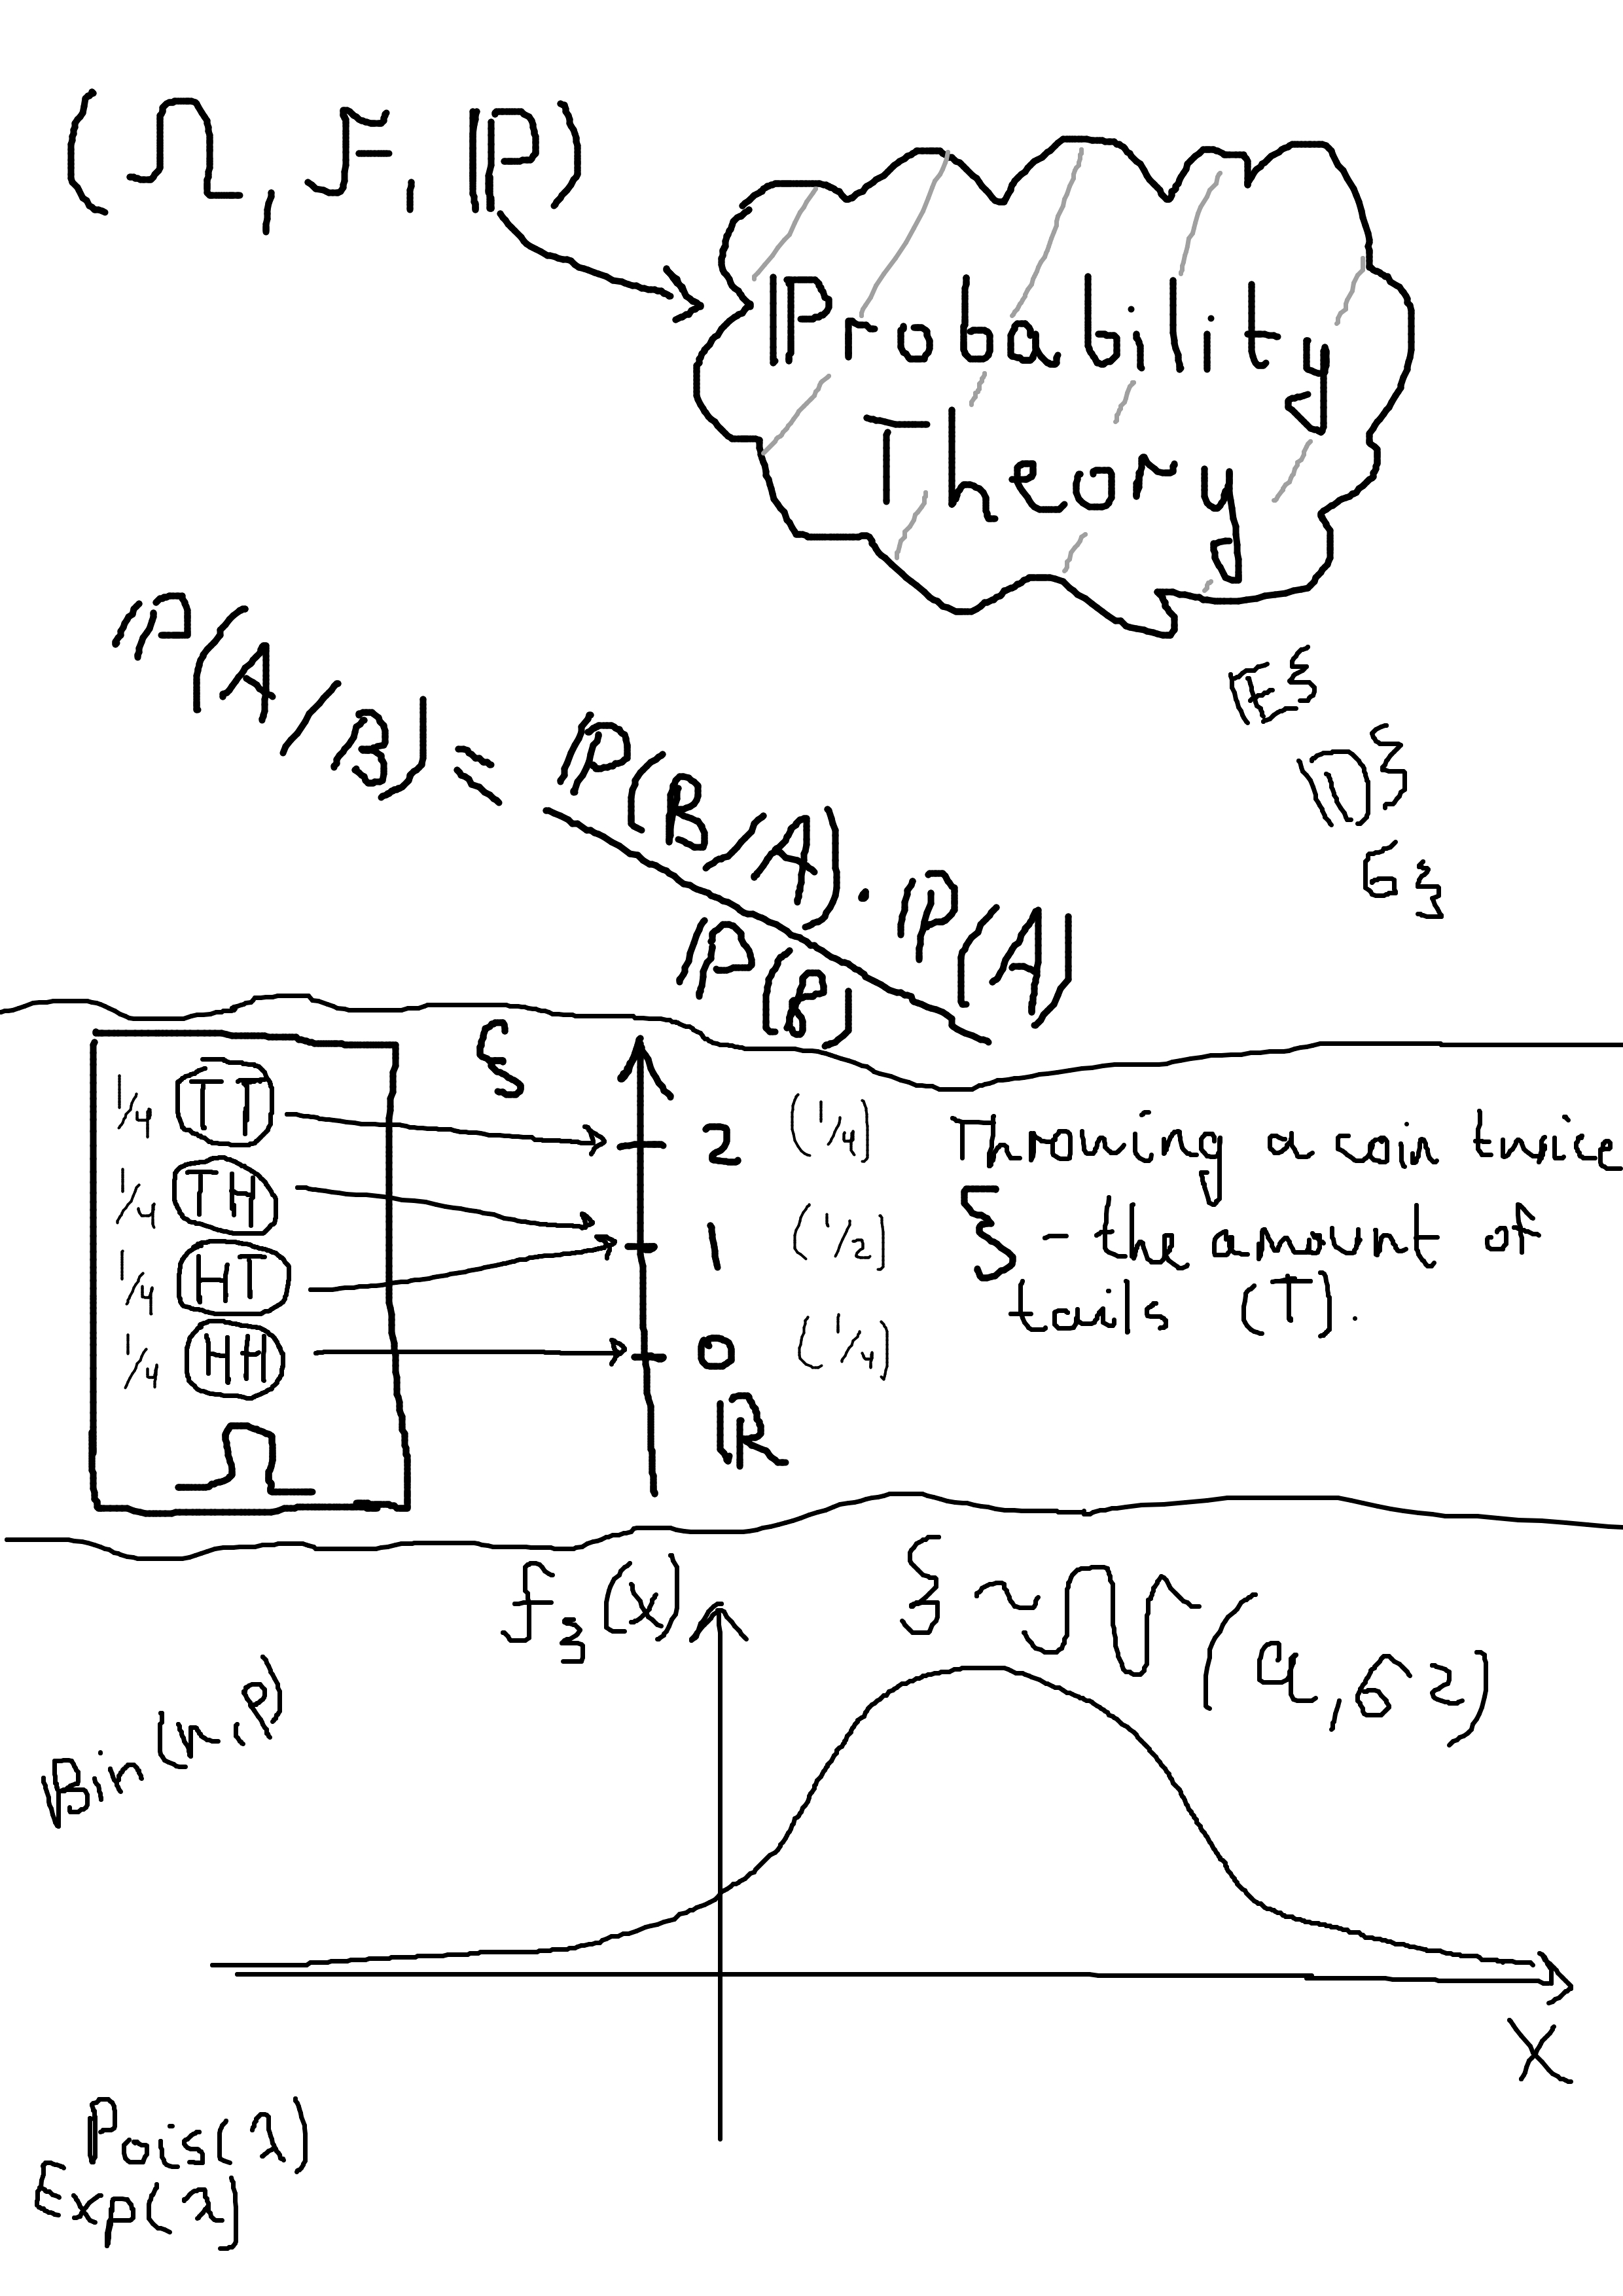
\includepdf[scale=1]{preview.jpg}
\thispagestyle{empty}
\tableofcontents
\newpage

\section{Класи множин}
\subsection{Основні класи множин}
\begin{definition}
Задано $X$ -- деяка множина та $\mathcal{K} \subset 2^X$ -- клас підмножин.\\
Непорожній клас $\mathcal{K}$ називається \textbf{кільцем}, якщо
\begin{align*}
\forall A,B \in \mathcal{K}: A \cup B \in \mathcal{K} \\
\forall A,B \in \mathcal{K}: A \setminus B \in \mathcal{K}
\end{align*}
\end{definition}

\begin{proposition}[Властивості кільця]
Задано $X$ та $\mathcal{K}$ -- кільце на цій множині. Тоді виконуються такі пункти:
\begin{enumerate}[nosep,wide=0pt,label={\arabic*)}]
\item $\emptyset \in \mathcal{K}$;
\item $\forall A,B \in \mathcal{K}: A \cap B \in \mathcal{K}$;
\item $\forall A_k \in \mathcal{K}, k = \overline{1,n}: \displaystyle\bigcup_{k=1}^n A_k \in \mathcal{K}, \displaystyle\bigcap_{k=1}^n A_k \in \mathcal{K}$.
\end{enumerate}
\end{proposition}

\begin{proof}
Покажемо виконання кожної властивості:
\begin{enumerate}[wide=0pt,label={\arabic*)}]
\item Оскільки $\mathcal{K}$ -- непорожня, то існує елемент $A \in \mathcal{K}$. Зокрема $A \setminus A = \emptyset \in \mathcal{K}$;
\item $\forall A,B \in \mathcal{K}: A \cap B = A \setminus (A \setminus B)$. За умовою кільця, $A \setminus B \in \mathcal{K}$ та $A \in \mathcal{K}$, а тому $A \cap B \in \mathcal{K}$.
\item Перше випливає з означення кільця, а друге випливає з властивості 2).
\end{enumerate}
Всі властивості доведені.
\end{proof}

\begin{definition}
Задано $X$ -- деяка множина та $\mathcal{A} \subset 2^X$ -- клас підмножин.\\
Непорожній клас $\mathcal{A}$ називається \textbf{алгеброю}, якщо
\begin{align*}
\mathcal{A} \text{ -- кільце} \\
X \in \mathcal{A}
\end{align*}
\end{definition}

\begin{definition}
Задано $X$ -- деяка множина та $\mathcal{P}$ -- клас підмножин.\\
Непорожній клас $\mathcal{P}$ назвемо \textbf{півкільцем}, якщо
\begin{align*}
\forall A,B \in \mathcal{P}: A \cap B \in \mathcal{P} \\
\forall A,B \in \mathcal{P}: A \setminus B = \bigsqcup_{i=1}^n C_i,\ C_i \in \mathcal{P}
\end{align*}
\end{definition}

\begin{remark}
$\emptyset \in \mathcal{P}$, тому що в силу непорожньості $A \in \mathcal{P}$, а тому за другою умовою, з одного боку, $A \setminus A = \displaystyle\bigsqcup_{i=1}^n C_i$ при $C_i \in \mathcal{P}$; а з іншого боку, $A \setminus A = \emptyset$. Тому рівність виконується лише при $C_i = \emptyset \in \mathcal{P}$.
\end{remark}

\begin{example}
Розглянемо $\mathcal{P}_1 = \{ (a,b] \mid a,b \in \mathbb{R} \}$ -- клас підмножин $\mathbb{R}$. Воно утворює півкільце.\\
Нехай $(a,b] \in \mathcal{P}_1$ та $(c,d] \in \mathcal{P}_1$. Тоді звідси $(a,b] \cap (c,d]$ кілька опцій:\\
1) $(a,b] \cap (c,d] = \emptyset \in \mathcal{P}_1$, якщо ці напівінтервали не перетинаються;\\
2) $(a,b] \cap (c,d] = (c,b] \in \mathcal{P}_1$, якщо (не втрачаючи загальності) $a < c < b < d$;\\
3) $(a,b] \cap (c,d] = (c,d] \in \mathcal{P}_1$, якщо (не втрачаючи загальності) $(c,d] \subset (a,b]$.
\begin{figure}[H]
\centering
\begin{tikzpicture}
\draw[->] (0,0)--(4.5,0);
\node at (0.5,0) {$($};
\node at (0.5,-0.5) {$a$};
\node at (1,0) {$]$};
\node at (1,-0.5) {$b$};
\node at (2,0) {$($};
\node at (2,-0.5) {$c$};
\node at (4,0) {$]$};
\node at (4,-0.5) {$d$};
\end{tikzpicture}
\qquad
\begin{tikzpicture}
\draw[->] (0,0)--(4.5,0);
\node at (0.5,0) {$($};
\node at (0.5,-0.5) {$a$};
\node at (3,0) {$]$};
\node at (3,-0.5) {$b$};
\node at (2,0) {$($};
\node at (2,-0.5) {$c$};
\node at (4,0) {$]$};
\node at (4,-0.5) {$d$};
\end{tikzpicture}
\qquad
\begin{tikzpicture}
\draw[->] (0,0)--(4.5,0);
\node at (2.5,0) {$($};
\node at (2.5,-0.5) {$c$};
\node at (3,0) {$]$};
\node at (3,-0.5) {$d$};
\node at (2,0) {$($};
\node at (2,-0.5) {$a$};
\node at (4,0) {$]$};
\node at (4,-0.5) {$b$};
\end{tikzpicture}
\caption*{Відповідно зліва направо: 1), 2), 3).}
\end{figure}
\noindent
Далі розглянемо $(a,b] \setminus (c,d]$. Знову кілька опцій:\\
1) $(a,b] \setminus (c,d] = (a,b]$, якщо ці напівінтервали не перетинаються;\\
2) $(a,b] \setminus (c,d] = (a,c]$, якщо (не втрачаючи загальності) $a < c < b < d$;\\
3) $(a,b] \setminus (c,d] = (a,c] \sqcup (b,d]$, якщо (не втрачаючи загальності) $(c,d] \subset (a,b]$.\\
Усі вони розклалися не неперетинне об'єднання елементів з $\mathcal{P}_1$.\\
Отже, $\mathcal{P}_1$ -- дійсно утворює півкільце.
\end{example}

\begin{theorem}
\label{product_of_semirings_is_semiring}
Задані $\mathcal{P}'$ та $\mathcal{P}''$ -- два півкільця на відповідних множинах $X_1,X_2$. Визначимо $\mathcal{P}' \times \mathcal{P}'' = \{ A_1 \times A_2 \mid A_1 \in \mathcal{P}', A_2 \in \mathcal{P}'' \}$. Тоді $\mathcal{P}' \times \mathcal{P}''$ буде півкільцем на множині $X_1 \times X_2$.
\end{theorem}

\begin{proof}
Нехай $A,B \in \mathcal{P}' \times \mathcal{P}''$, тобто $A = A_1 \times A_2$ та $B = B_1 \times B_2$, де $A_1,B_1 \in \mathcal{P}'$ та $A_2,B_2 \in \mathcal{P}''$.\\
$A \cap B = (A_1 \times A_2) \cap (B_1 \times B_2) = (A_1 \cap B_1) \times (A_2 \cap B_2)$.\\
Причому $A_1 \cap B_1 \in \mathcal{P}'$ та $A_2 \cap B_2 \in \mathcal{P}''$ за визначеннями півкілець. А за визначенням $\mathcal{P}' \times \mathcal{P}''$, звідси $A \cap B \in \mathcal{P}' \times \mathcal{P}''$.\\
$A \setminus B = [(A_1 \setminus B_1) \times A_2] \sqcup [(A_1 \cap B_1) \times (A_2 \setminus B_2)]$ (вправа: довести рівність).\\
Зауважимо, що $A_1 \setminus B_1 = \displaystyle\bigsqcup_{i=1}^n C_i$ та $A_2 \setminus B_2 = \displaystyle\bigsqcup_{k=1}^m D_k$, причому $C_i \in \mathcal{P}',D_k \in \mathcal{P}''$. Значить, рівність можна дописати:\\
$A \setminus B = \displaystyle\bigsqcup_{i=1}^n (C_i \times A_2) \sqcup \bigsqcup_{k=1}^m ((A_1 \cap B_1) \times D_k)$.\\
У нас записані елементи з $\mathcal{P}' \times \mathcal{P}''$, а сама множина $A \setminus B$ записалася як неперетинне об'єднання елементів з $\mathcal{P}' \times \mathcal{P}''$.\\
Висновок: $\mathcal{P}' \times \mathcal{P}''$ задає півкільце на $X_1 \times X_2$.
\end{proof}

\begin{remark}
Зрозуміло, що твердження працює для скінченного числа півкілець.
\end{remark}

\begin{example}
Зокрема $\mathcal{P}_1$ -- півкільце на $\mathbb{R}$. Визначимо нову множну $\mathcal{P}_d = \left\{ \displaystyle\prod_{i=1}^d (a_i,b_i] \mid a_i,b_i \in \mathbb{R} \right\}$. Тоді $\mathcal{P}_d$ буде півкільцем множини $\mathbb{R}^d$, просто тому що $\mathcal{P}_d = \mathcal{P}_1 \times \dots \times \mathcal{P}_1$.
\end{example}

\begin{remark}
Будь-яке кільце $\mathcal{K}$ -- автоматично півкільце.\\
Адже перша умова виконана за властивістю 2) кільця. А також за означенням, $A \setminus B = A \setminus B$, де $A \setminus B \in \mathcal{K}$ -- тобто цей елемент розписали не неперетинне об'єднання з одного елемента з даного класу.
\end{remark}

\begin{definition}
Задано $X$ -- деяка множина та $\sigma \mathcal{K} \subset 2^X$ -- клас підмножин.\\
Непорожній клас $\sigma \mathcal{K}$ називається \textbf{$\sigma$-кільцем}, якщо
\begin{align*}
\forall A_n \in \sigma\mathcal{K}, n \geq 1: \bigcup_{n=1}^\infty A_n \in \sigma\mathcal{K} \\
\forall A,B \in \sigma\mathcal{K}: A \setminus B \in \sigma\mathcal{K}
\end{align*}
\end{definition}

\begin{proposition}[Властивості $\sigma$-кільця]
Задано $X$ та $\sigma\mathcal{K}$ -- $\sigma$-кільце на цій множині. Тоді виконуються такі пункти:
\begin{enumerate}[nosep,wide=0pt,label={\arabic*)}]
\item $\sigma \mathcal{K}$ -- буде (просто) кільецм;
\item $\forall A_n \in \sigma\mathcal{K}, n \geq 1: \displaystyle\bigcap_{n=1}^\infty A_n \in \sigma\mathcal{K}$.
\end{enumerate}
\end{proposition}

\begin{proof}
Покажемо виконання кожної властивості:
\begin{enumerate}[wide=0pt,label={\arabic*)}]
\item Візьмемо $A,B \in \sigma \mathcal{K}$, тоді звідси $A \cup B = A \cup B \cup B \cup B \cup \dots \in \sigma \mathcal{K}$.
\item $\forall A_n \in \sigma \mathcal{K}, n \geq 1: \displaystyle\bigcap_{n=1}^\infty A_n = A_1 \setminus \bigcup_{n=2}^\infty (A_1 \setminus A_n) \in \sigma \mathcal{K}$.
\end{enumerate}
Всі властивості доведені.
\end{proof}

\begin{definition}
Задано $X$ -- деяка множина та $\sigma\mathcal{A} \subset 2^X$ -- клас підмножин.\\
Непорожній клас $\sigma\mathcal{A}$ називається $\sigma$-\textbf{алгеброю}, якщо
\begin{align*}
\sigma\mathcal{A} \text{ -- $\sigma$-кільце} \\
X \in \sigma\mathcal{A}
\end{align*}
\end{definition}

\begin{definition}
Задамо послідовність множин $\{A_n, n \geq 1\}$.\\
Вона буде називатися \textbf{зростаючою}, якщо $A_{n+1} \supset A_n$. \\
У такому випадку ми позначимо $\displaystyle\bigcup_{n=1}^\infty A_n \overset{\text{def.}}{=} \lim_{n \to \infty} A_n$.\\
Вона буде називатися \textbf{спадною}, якщо $A_{n+1} \subset A_n$. \\
У такому випадку ми позначимо $\displaystyle\bigcap_{n=1}^\infty A_n \overset{\text{def.}}{=} \lim_{n \to \infty} A_n$.\\
Обидві послідовності множин будемо називати \textbf{монотонними}.
\end{definition}

\begin{definition}
Задано $X$ -- деяка множина та $\mathcal{M} \subset 2^X$ -- клас підмножин.\\
Непорожній клас $m$ називається \textbf{монотонним}, якщо
\begin{align*}
\forall \{A_n \in \mathcal{M}, n \geq 1\} \text{ -- монотонна}: \displaystyle\lim_{n \to \infty} A_n \in \mathcal{M}
\end{align*}
\end{definition}

\begin{theorem}
\label{monotonic_ring_is_sigma_ring}
Задано $\mathcal{H}$ -- кільце та монотонний клас множин $X$. Тоді $\mathcal{H}$ -- $\sigma$-кільце.
\end{theorem}

\begin{proof}
Нехай $A_n \in \mathcal{H}, n \geq 1$. Розглянемо послідовність множин $\{B_n, n \geq 1\}$, що задається таким чином:\\
$B_1 = A_1$,\ $B_1 = A_1 \cup A_2$,\ $B_3 = A_1 \cup A_2 \cup A_3$, \dots\\
Зауважимо, що $\{B_n \overset{!}{\in} \mathcal{H}\}$ зростає, а в силу монотонності, звідси $\displaystyle\bigcup_{n=1}^\infty B_n = \bigcup_{n=1}^\infty A_n \in \mathcal{P}$.\\
Ну й якщо $A,B \in \mathcal{H}$, то за означенням кільце, $A \setminus B \in \mathcal{H}$.\\
Висновок: $\mathcal{H}$ -- $\sigma$-кільце.
\end{proof}

\subsection{Породжені класи множин}
\begin{definition}
Задано $X$ -- множина та $\mathcal{H}$ -- непорожня множина.\\
\textbf{Кільцем, породженим класом $\mathcal{H}$}, називається така множина:
\begin{align*}
k(\mathcal{H}) \overset{\text{def.}}{=} \bigcap_{\substack{\mathcal{K}_\alpha \supset \mathcal{H} \\ \mathcal{K}_\alpha \text{ -- кільце}}} \mathcal{K}_\alpha
\end{align*}
\textbf{$\sigma$-кільцем, породженим класом $\mathcal{H}$}, називається така множина:
\begin{align*}
\sigma k(\mathcal{H}) \overset{\text{def.}}{=} \bigcap_{\substack{(\sigma\mathcal{K})_\alpha \supset \mathcal{H} \\ (\sigma\mathcal{K})_\alpha \text{ -- $\sigma$-кільце}}} (\sigma\mathcal{K})_\alpha
\end{align*}
\textbf{Алгеброю, породженим класом $\mathcal{H}$}, називається така множина:
\begin{align*}
a(\mathcal{H}) \overset{\text{def.}}{=} \bigcap_{\substack{\mathcal{A}_\alpha \supset \mathcal{H} \\ \mathcal{A}_\alpha \text{ -- алгебра}}} \mathcal{A}_\alpha
\end{align*}
\textbf{$\sigma$-алгеброю, породженим класом $\mathcal{H}$}, називається така множина:
\begin{align*}
\sigma a(\mathcal{H}) \overset{\text{def.}}{=} \bigcap_{\substack{(\sigma\mathcal{A})_\alpha \supset \mathcal{H} \\ (\sigma\mathcal{A})_\alpha \text{ -- $\sigma$-алгебра}}} (\sigma\mathcal{A})_\alpha
\end{align*}
\textbf{Монотонним класом, породженим класом $\mathcal{H}$}, називається така множина:
\begin{align*}
m(\mathcal{H}) \overset{\text{def.}}{=} \bigcap_{\substack{\mathcal{M}_\alpha \supset \mathcal{H} \\ \mathcal{M}_\alpha \text{ -- монотонний клас}}} \mathcal{M}_\alpha
\end{align*}
\end{definition}

\begin{remark}
Я зосереджуся лише на породжених кільцях. Нижче будуть зазначені властивості породжених кілець -- аналогічно ті властивості переписуються для інших породжених класів.
\end{remark}

\begin{remark}
Зауважимо, що $k(\mathcal{H}) \neq \emptyset$. Оскільки $\mathcal{K}_\alpha$ -- кільця, то тоді $\emptyset \in \mathcal{K}_\alpha$ при всіх $\alpha$, а тому $\emptyset \in k(\mathcal{H})$.
\end{remark}

\begin{proposition}[Властивості породженого кільця]
Задано $X$ -- множина та $\mathcal{H}$ -- непорожня множина. Тоді виконуються такі пункти:
\begin{enumerate}[nosep, wide=0pt, label={\arabic*)}]
\item $k(\mathcal{H})$ -- дійсно, кільце;
\item $k(\mathcal{H}) \supset \mathcal{H}$;
\item Нехай $\mathcal{K}$ -- якесь кільце, де $\mathcal{K} \supset \mathcal{H}$. Тоді звідси $\mathcal{K} \supset k(\mathcal{H})$.
\end{enumerate}
\end{proposition}

\begin{proof}
Доведемо виконання всіх пунктів:
\begin{enumerate}[wide=0pt, label={\arabic*)}]
\item Нехай $A,B \in k(\mathcal{H})$, тобто звідси $A,B \in \mathcal{K}_\alpha$ при всіх $\alpha$. Оскільки $\mathcal{K}_\alpha$ -- кільце при всіх $\alpha$, то звідси $A \cup B \in \mathcal{K}_\alpha$ при всіх $\alpha$. Тобто звідси $A \cup B \in k(\mathcal{H})$.\\
Аналогічно доводимо, що $A \setminus B \in k(\mathcal{H})$.

\item це випливає з того, що всі $\mathcal{K}_\alpha \supset \mathcal{H}$, а далі перетнути треба по $\alpha$.

\item Маємо $\mathcal{K} \supset \mathcal{H}$ -- якесь кільце. Тоді $\mathcal{K}$ бере участь у перетинні всіх кілець в $k(\mathcal{H})$, просто за умовою такого кільця. Значить, $k(\mathcal{H}) = \displaystyle\bigcap_{\substack{\mathcal{K}_\alpha \supset \mathcal{H} \\ \mathcal{K}_\alpha \text{ -- кільце} \\ \mathcal{K}_\alpha \neq \mathcal{K}}} \mathcal{K}_\alpha \cap \mathcal{K} \subset \mathcal{K}$.
\end{enumerate}
Всі властивості доведені.
\end{proof}

\begin{corollary}
$k(\mathcal{H})$ -- найменше кільце, що містить $\mathcal{H}$ -- непорожній клас підмножин $X$.
\end{corollary}

\begin{theorem}
\label{ring_generated_by_semiring}
Задано $\mathcal{P}$ -- півкільце. Тоді $k(\mathcal{P}) = \{ A_1 \sqcup \dots \sqcup A_k \mid A_n \in \mathcal{P} \}$.
\end{theorem}

\begin{proof}
Для спрощення позначимо клас множин $\mathcal{L} = \{A_1 \sqcup \dots \sqcup A_k \mid A_n \in \mathcal{P}\}$. Хочемо довести, що $k(\mathcal{P}) = \mathcal{L}$.\\
$\mathcal{L} \subset k(\mathcal{P})$.\\
Дійсно, якщо $D \in \mathcal{D}$, то звідси $D = A_1 \sqcup \dots \sqcup A_k$, де всі $A_n \in \mathcal{P}$. Але $\mathcal{P} \subset k(\mathcal{P})$, звідси, за означенням кільця, $D \in k(\mathcal{H})$.\\
$\mathcal{L} \supset k(\mathcal{P})$.\\
Зрозуміло цілком, що $\mathcal{L} \supset \mathcal{P}$. Нам треба довести, що $\mathcal{L}$ буде кільцем -- і тоді звідси, за властивістю 3) породжених кілець, $\mathcal{L} \supset k(\mathcal{P})$.\\
Нехай $A,B \in \mathcal{L}$, тобто звідси $A = \displaystyle\bigsqcup_{i=1}^n C_i,\ B = \displaystyle\bigsqcup_{k=1}^m D_k$ та всі $C_i, D_k \in \mathcal{P}$.\\
$A \sqcup B \in \mathcal{L}$ (це якщо $A \cap B = \emptyset$, а тому звідси кожний $C_i \cap D_k = \emptyset$). Дійсно, $A \sqcup B = C_1 \sqcup \dots \sqcup D_m$, всі ці елементи з $\mathcal{P}$.\\
$A \cap B \in \mathcal{L}$. Дійсно, $A \cap B = \displaystyle\bigsqcup_{\substack{1 \leq i \leq n \\ 1 \leq k \leq m}} (C_i \cap D_k)$, причому кожний $C_i \cap D_k \in \mathcal{P}$ за означенням півкільця.\\
$A \setminus B \in \mathcal{L}$ (перша вимога кільця). Спочатку зауважимо, що $A \setminus B = \displaystyle\bigsqcup_{i=1}^n (C_i \setminus B)$, а далі кожний $C_i \setminus B = \displaystyle\bigcap_{k=1}^m (C_i \setminus D_k)$. Але оскільки $C_i,D_k \in \mathcal{P}$, то тоді $C_i \setminus D_k = \displaystyle\bigsqcup_{r=1}^{s_{ik}} G_r$ та кожний $G_r \in \mathcal{P}$. Звідси випливає $C_i \setminus D_k \in \mathcal{L}$, а тому далі $C_i \setminus B \in \mathcal{L}$ як перетин, а після $A \setminus B \in \mathcal{L}$ як диз'юнктивне об'єднання.\\
$A \cup B \in \mathcal{L}$ (друга вимога кільця). Дійсно, розпишемо $A \cup B = (A \setminus B) \sqcup (A \cap B) \sqcup (B \setminus A)$.\\
Отже, нарешті довели, що $\mathcal{L}$ утворює кільце, що завершує доведення.
\end{proof}

\begin{example}
Зокрема $k(\mathcal{P}_1) = \displaystyle\left\{ \bigsqcup_{k=1}^n (a_k,b_k] \mid (a,k,b_k] \subset \mathbb{R} \right\}$. Аналогічно визначається $k(\mathcal{P}_d)$.
\end{example}

\begin{theorem}
\label{monotonic_class_generated_by_ring_is_sigma_ring_generated_by_ring}
Задано $\mathcal{K}$ -- кільце. Тоді $m(\mathcal{K}) = \sigma k(\mathcal{K})$.
\end{theorem}

\begin{proof}
$m(\mathcal{K}) \subset \sigma k(\mathcal{K})$.\\
Дійсно, $\sigma k(\mathcal{K}) \supset \mathcal{K}$, за властивістю породжених $\sigma$-кілець. Також $\sigma k(\mathcal{K})$ буде монотонним класом, тому що під $\displaystyle\lim_{n \to \infty} A_n, A_n \in \mathcal{K}$, ми маємо на увазі зліченне об'єдання або перетин, що допустимо. Звідси випливає, що $\sigma k(\mathcal{K}) \supset m(\mathcal{K})$.
\bigskip \\
$m(\mathcal{K}) \supset \sigma k(\mathcal{K})$.\\
Маємо $m(\mathcal{K}) \supset \mathcal{K}$, за властивістю породжених монотонних класів. Нам треба довести, що $m(\mathcal{K})$ буде $\sigma$-кільцем -- і тоді звідси $m(\mathcal{K}) \supset \sigma k(\mathcal{K})$. А щоб довести, що $m(\mathcal{K})$ буде $\sigma$-кільцем, достатньо за \thref{monotonic_ring_is_sigma_ring} довести, що $m(\mathcal{K})$ -- просто кільце.\\
Нехай $A \in m(\mathcal{K})$. Розглянемо клас множин $\mathcal{L}(A) = \{B \subset X \mid A \cup B, A \setminus B, B \setminus A \in m(\mathcal{K})\}$. Покажемо, що це -- монотонний клас.\\
Нехай $C_n \in \mathcal{L}(A)$, причому $C_n$ зростає. Позначимо $\displaystyle\bigcup_{n=1}^\infty C_n = C$. Тоді\\
$A \cup C = \displaystyle\bigcup_{n=1}^\infty (A \cup C_n)$, причому $(A \cup C_n) \in m(\mathcal{K})$ (за визначенням $\mathcal{L}(A)$), а також $(A \cup C_n)$ монотонно зростає до $(A \cup C)$, звідси $A \cup C \in m(\mathcal{K})$.\\
$A \setminus C = \displaystyle\bigcap_{n=1}^\infty (A \setminus C_n)$, причому $A \setminus C_n \in m(\mathcal{K})$ (за визначенням $\mathcal{L}(A)$), а також $(A \setminus C_n)$ монотонно спадає до $(A \setminus C)$, звідси $A \setminus C \in m(\mathcal{K})$.\\
$C \setminus A = \displaystyle\bigcup_{n=1}^\infty (C_n \setminus A)$, причому $C_n \setminus A \in m(\mathcal{K})$ (за визначенням $\mathcal{L}(A)$), а також $(A \setminus C_n)$ монотонно зростає до $(C \setminus A)$, звідси $C \setminus A \in m(\mathcal{K})$.\\
Із цих трьох випливає, що $C \in \mathcal{L}(A)$. Цілком аналогічно доводиться, що якщо $C_n \in \mathcal{L}(A)$ та $C_n$ спадає, то $C = \displaystyle\bigcap_{n=1}^\infty C_n \in \mathcal{L}(A)$ (тут $A \in \mathcal{K}$!).\\
Нехай $A \in \mathcal{K}$. Оскільки $\mathcal{K}$ -- це кільце, то для кожної $B \in \mathcal{K}$ отримаємо $A \cup B, A \setminus B, B \setminus A \in \mathcal{K}$, а звідси $A \cup B, A \setminus B, B \setminus A \in m(\mathcal{K})$. Із цього випливає, що $B \in \mathcal{L}(A)$. Тобто із цього випливає, що для фіксованого $A \in \mathcal{K}$ маємо $\mathcal{K} \subset \mathcal{L}(A)$. Але оскільки $\mathcal{L}(A)$ -- монотонний, то $m (\mathcal{K}) \subset \mathcal{L}(A)$.\\
Отже, для фіксованого $A \in \mathcal{K}$ і для будь-якої множини $B \in m(\mathcal{K})$, маємо $B \in \mathcal{L}(A)$, тобто $A \cup B, A \setminus B, B \setminus A \in m(\mathcal{K})$. Але конкретно цей запис означає, що $A \in \mathcal{L}(B)$. Тобто $A \in \mathcal{K} \implies A \in \mathcal{L}(B)$, а тому звідси $\mathcal{K} \subset \mathcal{L}(B)$. Аналогічно отримаємо $m(\mathcal{K}) \subset \mathcal{L}(B)$ (тут $A \in m(\mathcal{K})$! Важлива різниця!).\\
Тепер нехай $A \in m(\mathcal{K})$, тоді $A \in \mathcal{L}(B)$. Це означає, що $A \cup B, A \setminus B \in m(\mathcal{K})$. Дана штука виконується для будь-яких $A,B \in m(\mathcal{K})$, що й доводить означення кільця.
\end{proof}

\subsection{Борельові множини}
\begin{definition}
Задано $(X,\rho)$ -- метричний простір та $\mathcal{G}$ -- набір усіх відкритих підмножин $X$.\\
\textbf{Борельовою $\sigma$-алгеброю} в $X$ називається наступна $\sigma$-алгебра:
\begin{align*}
\mathcal{B}(X) \overset{\text{def.}}{=} \sigma a(\mathcal{G})
\end{align*}
Тобто ми взяли клас відкритих підмножин в $Y$ та породили $\sigma$-алгебру.\\
Всі множини з $\mathcal{B}(X)$ називаються \textbf{борельовими}.
\end{definition}

\begin{remark}
Переважно будемо користуватися стандартною метрикою, де це можливо.
\end{remark}

\begin{example}
Розглянемо кілька прикладів борельових множин:\\
1) Якщо $U$ -- відкрита, то $U$ -- борельова.\\
Дійсно, $U$ -- відкрита, тобто $U \in \mathcal{G}$, але звідси $U \in \sigma a(\mathcal{G}) = \mathcal{B}(X)$ за властивістю породжених $\sigma$-алгебр.
\bigskip \\
2) Якщо $V$ -- замкнена, то $U$ -- борельова.\\
Дійсно, $V$ -- замкнена, тому $X \setminus V$ -- відкрита. Розпишемо $V = X \setminus (X \setminus V)$. У нас множина $X \setminus V$ уже борельова за 1). Також $X$ -- відкрита множина, а тому знову борельова. Значить, $X, X \setminus V \in \sigma a(\mathcal{G}) \implies X \setminus (X \setminus V) = V \in \sigma a(\mathcal{G}) = \mathcal{B}(X)$ -- борельова.
\bigskip \\
3. Одноточкова множина $\{x\}$ -- борельова.\\
Дійсно, $\{x\}$ -- замкнена множина, а тому за 2), уже борельова.
\bigskip \\
4. Скінченні, зліченні множини -- всі вони борельові.\\
Усі ці множини отримуються через одноточкові множин, а далі 3).
\end{example}

\begin{theorem}
Для півкільця $\mathcal{P}_d$ підмножин $\mathbb{R}^d$ виконується $\sigma k(\mathcal{P}_d) = \sigma a(\mathcal{P}_d) = \mathcal{B}(\mathbb{R}^d)$.
\end{theorem}

\begin{proof}
$\sigma k(\mathcal{P}_d) = \sigma a(\mathcal{P}_d)$.\\
Дійсно, $\sigma a(\mathcal{P}_d) \supset \mathcal{P}_d$, але $\sigma$-алгебра уже є $\sigma$-кільцем, тому звідси $\sigma a(\mathcal{P}_d) \supset \sigma k(\mathcal{P}_d)$.\\
Далі $\sigma k(\mathcal{P}) \supset \mathcal{P}_d$, залишилося довести, що $\sigma k(\mathcal{P})$ утворює $\sigma$-алгебру -- і тоді $\sigma k(\mathcal{P}_d) \supset \sigma a(\mathcal{P}_d)$. \\
Для цього зауважимо, що $\mathbb{R}^d = \displaystyle\bigcup_{n =1}^\infty (-n,n]^d$, де всі $(-n,n]^d \in k(\mathcal{P}_d)$, а тому звідси $\mathbb{R}^d \in k(\mathcal{P}_d)$.
\bigskip \\
$\sigma a(\mathcal{P}_d) = \mathcal{B}(\mathbb{R}^d)$.\\
Спочатку покажемо, що $\mathcal{B}(\mathbb{R}^d) \supset \sigma a(\mathcal{P}_d)$. Щоб це довести, необіхдно довести, що $\mathcal{B}(\mathbb{R}^d) \supset \mathcal{P}_d$. А далі, зважаючи на той факт, що $\mathcal{B}(\mathbb{R}^d)$ утворює $\sigma$-алгебру, доведемо, що $\mathcal{B}(\mathbb{R}^d) \supset \sigma a(\mathcal{P}_d)$.\\
Нехай $A \in \mathcal{P}_d$, тобто $A = \displaystyle\prod_{i=1}^d (a_i,b_i]$. Зауважимо, що $(a_i,b_i] = \displaystyle\bigcap_{n=1}^\infty \left(a_i,b_i+\dfrac{1}{n}\right)$. Далі\\
$A = \displaystyle\prod_{i=1}^d \bigcap_{n=1}^\infty \left( a_i, b_i + \dfrac{1}{n} \right) = \bigcap_{n=1}^\infty \prod_{i=1}^d \left( a_i, b_i+\dfrac{1}{n}\right)$.\\
Декартів добуток відкритих множин -- відкрита, а кожна відкрита -- уже борельова. А оскільки там $\sigma$-алгебра, то допускається зліченний перетин, звідси $A \in \mathcal{B}(\mathbb{R}^d)$. Отже, $\mathcal{B}(\mathbb{R}^d) \supset \mathcal{P}_d$.\\
Нарешті, покажемо, що $\mathcal{B}(\mathbb{R}^d) \subset \sigma a(\mathcal{P}_d)$. Щоб це довести, треба довести, що $\sigma a(\mathcal{P}_d) \supset \mathcal{G}$, де $\mathcal{G}$ -- всі відкриті підмножини $\mathbb{R}^d$. Після цього ми отримуємо $\sigma a(\mathcal{P}_d) \supset \sigma a(\mathcal{G}) = \mathcal{B}(\mathbb{R}^d)$.\\
Отже, нехай $U \in \mathcal{G}$, тобто нехай $U$ -- відкрита множина. Запишемо її таким чином:\\
$U = \displaystyle\bigcup_{\substack{\prod_{i=1}^d (p_i,q_i] \subset U \\ p_i,q_i \in \mathbb{Q}}} \prod_{i=1}^d (p_i,q_i]$.\\
Якщо $\vec{x}$ лежить в цьому об'єднанні, то тоді автоматично $\vec{x} \in U$.\\
Якщо $\vec{x} \in U$, то вона внутрішня, тож існує куля $B(\vec{x},\varepsilon) \subset U$. А там $\forall \vec{y}: \| \vec{x} - \vec{y} \| < \varepsilon$. Тобто звідси $|x_i-y_i| < \dfrac{\varepsilon}{\sqrt{d}} \implies y_i - \dfrac{\varepsilon}{\sqrt{d}} < x_i < y_i + \dfrac{\varepsilon}{\sqrt{d}}$. Між кожним з цих нерівностей можна знайти раціональні числа $p_i,q_i \in \mathbb{Q}$, тоді звідси $p_i < x_i < q_i$. Звідси $\vec{x} \in \displaystyle\prod_{i=1}^d (p_i,q_i]$. Але також важливо зауважити, що $\displaystyle\prod_{i=1}^d (p_i,q_i] \subset U$. Отже, $\vec{x}$ лежить в цьому об'єднанні.\\
Множина $U$ записалась як зліченне об'єднання елементів з $\mathcal{P}_d \subset \sigma a(\mathcal{P}_d$. Отже, звідси $U \in \sigma a(\mathcal{P}_d)$. Отже, $\mathcal{G} \subset \sigma a(\mathcal{P}_d)$.
\end{proof}
\newpage

\section{Міри}
\subsection{Основні функції множин}
\begin{definition}
Задано $X$ -- деяка множина та $\mathcal{H} \subset 2^X$ -- клас підмножин.\\
\textbf{Функцією множин} називатимемо відображення $f \colon \mathcal{H} \to (-\infty,+\infty]$. Ми будемо вважати надалі, що $-\infty$ неможливий.
\end{definition}

\begin{definition}
Задано функцію множин $f$ на $\mathcal{H} \subset 2^X$.\\
Функція множин $f$ називається \textbf{невід'ємною}, якщо
\begin{align*}
\forall A \in \mathcal{H}: f(A) \geq 0
\end{align*}
Функція множин $f$ називається \textbf{адитивною}, якщо
\begin{align*}
\forall A_1,\dots,A_k \in \mathcal{H}, \text{причому } \bigsqcup_{n=1}^k A_n \in \mathcal{H}: f\left( \bigsqcup_{n=1}^k A_n \right) = \sum_{n=1}^k f(A_n)
\end{align*}
Функція множин $f$ називається \textbf{$\sigma$-адитивною}, якщо
\begin{align*}
\forall A_1,A_2,\dots \in \mathcal{H}, \text{причому } \bigsqcup_{n=1}^\infty A_n \in \mathcal{H}: f\left( \bigsqcup_{n=1}^\infty A_n \right) = \sum_{n=1}^\infty f(A_n)
\end{align*}
Функція множин $f$ називається \textbf{напівадитивною}, якщо
\begin{align*}
\forall A_1,\dots,A_k \in \mathcal{H}, \text{причому } \bigcup_{n=1}^k A_n \in \mathcal{H}: f\left( \bigcup_{n=1}^k A_n \right) \leq \sum_{n=1}^k f(A_n)
\end{align*}
Функція множин $f$ називається \textbf{$\sigma$-напівадитивною}, якщо
\begin{align*}
\forall A_1,A_2,\dots \in \mathcal{H}, \text{причому } \bigcup_{n=1}^\infty A_n \in \mathcal{H}: f\left( \bigcup_{n=1}^\infty A_n \right) \leq \sum_{n=1}^\infty f(A_n)
\end{align*}
Функція множин $f$ називається \textbf{скінченною}, якщо
\begin{align*}
\forall A \in \mathcal{H}: f(A) < +\infty
\end{align*}
Функція множин $f$ називається \textbf{$\sigma$-скінченною}, якщо
\begin{align*}
\exists A_1,A_2, \dots \in \mathcal{H}: \bigcup_{n=1}^\infty A_n = X,\ f(A_n) < +\infty
\end{align*}
Функція множин $f$ називається \textbf{монотонною}, якщо
\begin{align*}
\forall A,B \in \mathcal{H}: A \subset B \implies f(A) \leq f(B)
\end{align*} 
\end{definition}

\begin{remark}
Домовленність: ми не будемо далі розглядати функції множин $f$, для яких $f \equiv +\infty$. Це означає, що в кожній функції множин $f$ буде існувати множина $A \in \mathcal{H}$, для якої $f(A) < +\infty$.
\end{remark}

\begin{remark}
Зрозуміло, що якщо функція множин скінченна, то вона автоматично $\sigma$-скінченна.
\end{remark}

\subsection{Означення міри}
\begin{definition}
Задано $\mathcal{P}$ -- півкільце.\\
\textbf{Мірою} ми називатимемо функцію множин $\lambda \colon \mathcal{P} \to [0,+\infty]$, де 
\begin{align*}
\lambda \text{ -- невід'ємною та $\sigma$-адитивна.}
\end{align*}
\end{definition}

\begin{proposition}[Властивості мір]
Задано $\lambda$ -- міра на півкільці $\mathcal{P}$. Тоді виконуються такі пункти:\\
\begin{enumerate}[nosep,wide=0pt,label={\arabic*)}]
\item $\lambda(\emptyset) = 0$;
\item $\lambda$ -- адитивна;
\item $\lambda$ -- монотонна;
\item $\lambda$ -- $\sigma$-напівадитивна;
\item $\forall A \in \mathcal{P}, \forall A_1,A_2,\dots \in \mathcal{P}: A \subset \displaystyle\bigcup_{n=1}^\infty A_n: \lambda(A) \leq \displaystyle\sum_{n=1}^\infty \lambda(A_n)$.
\end{enumerate}

\begin{proof}
Доведемо виконання всіх пунктів:
\begin{enumerate}[wide=0pt, label={\arabic*)}]
\item Тут на допомогу приходить узгодження в підпункті вище. У нас існує $A \in \mathcal{P}$, для якої $\lambda(A) < +\infty$. Розпишемо $A =  A \sqcup \emptyset \sqcup \emptyset \sqcup \dots$, причому $\emptyset \in \mathcal{P}$. Звідси, за $\sigma$-адитивністю, $\lambda(A) = \lambda(A) + \lambda(\emptyset) + \lambda(\emptyset) + \dots$ Але оскільки $\lambda(A) < +\infty$, то ряд збіжний, а для рівності треба вимагати $\lambda(\emptyset) = 0$.

\item Нехай $A_1,\dots,A_k \in \mathcal{P}$, причому $\displaystyle\bigcup_{n=1}^k A_n \in \mathcal{P}$. Тоді за $\sigma$-адитивністю міри та за властивістю 1),\\ $\displaystyle\lambda\left( \bigsqcup_{n=1}^\infty A_n \right) = \lambda(A_1 \sqcup \dots \sqcup A_n \sqcup \emptyset \sqcup \emptyset \sqcup \dots) = \lambda(A_1) + \dots + \lambda(A_n) + \lambda(\emptyset) + \dots = \sum_{n=1}^k \lambda(A_n)$.

\item Нехай $A,B \in \mathcal{P}$ таким чином, що $A \subset B$. Тоді звідси $B = (B \setminus A) \sqcup A$. На півкільці $A \setminus B = \displaystyle\bigsqcup_{i=1}^n C_i$ при $C_i \in \mathcal{P}$. Отже, звідси $B = \displaystyle\bigsqcup_{i=1}^n C_i \sqcup A$, а за властивістю 2) та невід'ємності міри, маємо \\ $\lambda(B) = \displaystyle\sum_{i=1}^n \lambda(C_i) + \lambda(A) \geq \lambda(A)$.

\item Нехай $A_1,A_2,\dots \in \mathcal{P}$, причому $\displaystyle\bigcup_{n=1}^\infty A_n \in \mathcal{P}$. Ми розглянемо $B_1 = A_1,\ B_2 = A_2 \setminus A_1,\ B_1 = A_3 \setminus (A_1 \cup A_2), \dots$ -- перейшли до системи неперетинних множин. Зауважимо, що $\displaystyle\bigsqcup_{n=1}^\infty B_n = \bigcup_{n=1}^\infty A_n \in \mathcal{P}$ (але при цьому неправильно казати, що $B_n \in \mathcal{P}$, тому юзаємо $\sigma$-адитивність!). Всі $A_n \in k(\mathcal{P})$, а тому звідси всі $B_n \in k(\mathcal{P})$, але тоді звідси $B_n = \displaystyle\bigsqcup_{i=1}^{i_n} C_{in}$ при $C_{in} \in \mathcal{P}$. Також зауважимо, що $A_n \setminus B_n \in k(\mathcal{P})$, а тому звідси $A_n \setminus B_n = \displaystyle\bigsqcup_{j=1}^{j_n} D_{jn}$ при $D_{jn} \in \mathcal{P}$.\\
Разом уже маємо $\displaystyle\bigcup_{n=1}^\infty A_n = \bigsqcup_{n=1}^\infty \bigsqcup_{i=1}^{i_n} C_{in} \in \mathcal{P}$, причому всі $C_{in} \in \mathcal{P}$, тому скористаємось $\sigma$-адитивністю:\\
$\displaystyle\lambda\left( \bigcup_{n=1}^\infty A_n \right) = \sum_{n=1}^\infty \sum_{i=1}^{i_n} \lambda(C_{in})$.\\
Водночас $A_n = A_n \setminus B_n \sqcup B_n = \displaystyle\bigsqcup_{j=1}^{j_n} D_{jn} \sqcup \bigsqcup_{i=1}^{i_n} C_{in} \in \mathcal{P}$, причому всі $C_{in},D_{jn} \in \mathcal{P}$ -- дійсно неперетинні всі між собою. Тому можна скористатися $\sigma$-адитивністю:\\
$\displaystyle\sum_{n=1}^\infty \lambda(A_n) = \sum_{n=1}^\infty \left( \sum_{j=1}^{j_n} \lambda(D_{jn}) + \sum_{i=1}^{i_n} \lambda(C_{in}) \right) \geq \sum_{n=1}^\infty \sum_{i=1}^{i_n} \lambda(C_{in}) = \lambda\left( \bigcup_{n=1}^\infty A_n \right)$.

\item Нехай $A \in \mathcal{P}$, а також задано покриття $A \subset \displaystyle\bigcup_{n=1}^\infty A_n$, де $A_n \in \mathcal{P}$. Зауважимо, що $A = A \cap \displaystyle\bigcup_{n=1}^\infty A_n = \bigcup_{n=1}^\infty (A \cap A_n)$, де $A \in \mathcal{P}$, а також $A \cap A_n \in \mathcal{P}$ за означенням півкільця. Тоді за 4),\\
$\displaystyle\lambda(A) = \lambda\left( \bigcup_{n=1}^\infty (A \cap A_n) \right) \leq \sum_{n=1}^\infty \lambda(A \cap A_n) \leq \sum_{n=1}^\infty \lambda(A_n)$.\\
\textit{До речі, властивість 5) -- це певне узагальнення властивості 4), тобто $\sigma$-напівадитивності.}
\end{enumerate} 
Всі властивості доведені.
\end{proof}
\end{proposition}

\begin{remark}
Якби $\lambda$ була невід'ємною та просто адитивною, то властивості 1),3),4),5) також би виконувалися, тільки там скінченна кількість замість зліченної.
\end{remark}

\begin{corollary}
Якщо $\lambda$ задана на кільці $\mathcal{K}$, то $\forall A,B \in \mathcal{K}: A \subset B: \lambda(A \setminus B) - \lambda(A) - \lambda(B)$.\\
\textit{Вказівка: $A \sqcup (B \setminus A) = B$, у цьому випадку $B \setminus A \in \mathcal{K}$, тому все легітимно.}
\end{corollary}

\begin{theorem}[Неперервність міри знизу]
Задано $\lambda$ -- міра уже на кільці $\mathcal{K}$. Нехай задана зростаюча послідовність $\{A_n \in \mathcal{K}, n \geq 1\}$, причому $\displaystyle\lim_{n \to \infty} A_n \in \mathcal{K}$. Тоді $\displaystyle\lambda\left(\lim_{n \to \infty} A_n\right) = \lim_{n \to \infty} \lambda(A_n)$.
\end{theorem}

\begin{proof}
Розглянемо $B_1 = A_1,\ B_2 = A_2 \setminus A_1,\ B_3 = A_3 \setminus A_2, \dots$ -- система неперетинних множин в силу зростання $\{A_n\}$. Зауважимо, що всі $B_n \in \mathcal{K}$, а також $\displaystyle\bigsqcup_{n=1}^\infty B_n = \bigcup_{n=1}^\infty A_n \in \mathcal{K}$. Тоді\\
$\displaystyle\lambda\left(\lim_{n \to \infty} A_n\right) = \lambda\left( \bigsqcup_{n=1}^\infty B_n \right) = \sum_{n=1}^\infty \lambda(B_n) = \\ =\lim_{j \to \infty} \sum_{n=1}^j \lambda(B_n) = \lim_{j \to \infty} (\lambda(A_1) + \lambda(A_2) - \lambda(A_1) + \lambda(A_3) - \lambda(A_2) + \dots + \lambda(A_j) - \lambda(A_{j-1})) = \lim_{j \to \infty} \lambda(A_j)$.\\
Мабуть, окремо зауважу, що в сумі я скористався наслідком вище.
\end{proof}

\begin{theorem}[Неперервність міри зверху]
Задано $\lambda$ -- міра уже на кільці $\mathcal{K}$. Нехай спадна зростаюча послідовність $\{A_n \in \mathcal{K}, n \geq 1\}$, причому $\displaystyle\lim_{n \to \infty} A_n \in \mathcal{K}$, а також $\lambda(A_1) < +\infty$! Тоді $\displaystyle\lambda\left(\lim_{n \to \infty} A_n\right) = \lim_{n \to \infty} \lambda(A_n)$.
\end{theorem}

\begin{proof}
Позначимо $A = \displaystyle\bigcap_{n=1}^\infty A_n$ та розглянемо послідовність $\{C_n \in \mathcal{K}, n \geq 1\}$ як $C_n = A_1 \setminus A_n$. Тепер послідовність зростає, при цьому $\displaystyle\bigcup_{n=1}^\infty C_n = A_1 \setminus A \in \mathcal{K}$. Тоді за неперервністю міри знизу,\\
$\lambda(A_1 \setminus A) = \displaystyle\lambda\left( \bigcup_{n=1}^\infty C_n \right) = \lim_{n \to \infty} \lambda\left(C_n\right) = \lim_{n \to \infty} \lambda(A_1 \setminus A_n)$.\\
Скорситавшись зауваженням вище, а також фактом, що $\lambda(A_1) < +\infty$, маємо\\
$\displaystyle\lambda(A_1) - \lambda(A) = \lambda(A_1) - \lim_{n \to \infty} \lambda(A_n) \implies \lambda(A) = \lambda\left( \lim_{n \to \infty} A_n \right) = \lim_{n \to \infty} \lambda(A_n)$.
\end{proof}

\begin{example}
Наведу приклад, де умова $\lambda(A_1) < +\infty$ є дуже важливою.\\
Розглянемо міру $\lambda(A) = \card (A \cap \mathbb{Z})$ на $2^{\mathbb{R}}$. Далі розглянемо спадну послідовність $\{ [n,+\infty), n \geq 1 \}$, причому в цьому випадку $\lambda([1,+\infty)) = \card \mathbb{N} = +\infty$. Тоді\\
$\displaystyle\lambda\left( \lim_{n \to \infty} [n,+\infty) \right) = \lambda\left( \bigcap_{n=1}^\infty [n,+\infty) \right) = \lambda(\emptyset) = 0$.\\
$\displaystyle\lim_{n \to \infty} \lambda([n,+\infty)) = \lim_{n \to \infty} \card (\mathbb{N} \setminus \{1,2,\dots,n\}) = +\infty$.\\
Отже, $\displaystyle\lambda\left( \lim_{n \to \infty} [n,+\infty) \right) \neq \lim_{n \to \infty} \lambda([n,+\infty))$ у даному випадку.
\end{example}

\subsection{Про міру Жордана}
Із курсу математичного аналізу відомо, що з себе представляє міра Жордана та клас вимірних множин $\mathcal{K}_d$. Даний контент можна подивитися в іншому пдф більш детально. Однак я зазначу, що міра Жордана $m$ -- ще не міра в сенсі означення, що було задано вище. Нам бракує лише $\sigma$-адитивності. Це питання розв'яжеться згодом.

\begin{lemma}
Нехай $A \in \mathcal{K}_d$. Тоді $\forall \varepsilon > 0: \exists F_\varepsilon, U_\varepsilon \in \mathcal{K}_d$ -- відповідно замкнена та відкрита множина: $\begin{cases} m(A) - m(F_\varepsilon) < \varepsilon \\ m(U_\varepsilon) - m(A) < \varepsilon \end{cases}$. Причому до всього цього $F_\varepsilon \subset A \subset U_\varepsilon$.\\
Тобто вимірну за Жорданом множину можна наблизити замкненим всередині множиною та відкритою зовні множиною.
\end{lemma}

\begin{proof}
I. \textit{Існування замкненої множини}.\\
$A$ -- вимірна за Жорданом, тоді $m(A) = \displaystyle\sup_{n \geq 0} m(F_{(n)})$, тоді існує $N$, для якого $m(F_{(N)}) > m(A) - \varepsilon$. Покладемо $F_\varepsilon = F_{(N)} \subset A$. Тоді звідси миттєво $m(A) - m(F_\varepsilon) < \varepsilon$. Ясно, що $F_\varepsilon$ вимірна за Жорданом.
\bigskip \\
II. \textit{Існування відкритої множини}.\\
Знову $A$ вимірна за Жорданом, то $m(A) = \displaystyle\inf_{n \geq 0} m(F^{(n)})$, тоді існує $\tilde{N}$, для якого $m(F^{(\tilde{N})}) < m(A) + \dfrac{\varepsilon}{2}$. У нас зараз $F^{(\tilde{N})} \supset A$, але поки що замкнена множина.\\
Згадаємо, що $F^{(\tilde{N})}$ складається зі скінченного об'єднання брусів вигляду $R = \displaystyle\prod_{i=1}^d \left[ \dfrac{k_i}{2^{\tilde{N}}}, \dfrac{k_i+1}{2^{\tilde{N}}} \right]$. Нехай $\delta > 0$ та замінимо замкнені бруси $R$ на відкриті бруси $R(\delta) =\displaystyle \prod_{i=1}^d \left( \dfrac{k_i}{2^{\tilde{N}}} - \delta, \dfrac{k_i+1}{2^{\tilde{N}}}+\delta \right)$. Зрозуміло, що $R(\delta) \supset R$, а тому звідси $F^{(\tilde{N})}(\delta) \supset F^{(\tilde{N})}$, де ось $F^{(\tilde{N})}(\delta)$ -- об'єднання відкритих брусів. Оскільки $m$ -- монотонна міра, то $m(F^{(\tilde{N})}) \leq m(F^{(\tilde{N})}(\delta))$. Звідси маємо наступне:\\
$m(F^{(\tilde{N})}) \leq m(F^{(\tilde{N})}(\delta)) \overset{m \text{ -- напівадитивна}}{\leq} \displaystyle\sum m(R(\delta)) = \sum \prod_{i=1}^d \left( \dfrac{k_i+1}{2^{\tilde{N}}} + \delta - \left(\dfrac{k_i}{2^{\tilde{N}}} - \delta  \right)\right) = \\ = \sum \left( \dfrac{1}{2^{\tilde{N}}} + 2 \delta \right)^d \xrightarrow{\delta \to 0} \sum \left( \dfrac{1}{2^{\tilde{N}}} \right)^d = \sum \prod_{i=1}^d \left[ \dfrac{k_i+1}{2^{\tilde{N}}} - \dfrac{k_i}{2^{\tilde{N}}} \right] = \sum m(R) = m(F^{(\tilde{N})})$.\\
Значить, звідси існує $\delta_1 > 0$, для якого $m(F^{(\tilde{N})}(\delta_1)) - m(F^{(\tilde{N})}) < \dfrac{\varepsilon}{2}$.\\
Нарешті, покладемо $U_\varepsilon = F^{(\tilde{N})}(\delta_1) \supset F^{(\tilde{N})} \supset A$. Ясно, що це відкрита множина (як об'єднання відкритих) та вимірна за Жорданом. Тоді звідси\\
$m(U_\varepsilon) - m(A) = (m(U_\varepsilon) - m(F^{(\tilde{N})})) + (m(F^{(\tilde{N})}) - m(A)) < \varepsilon$.
%TODO see text and format brackets
\end{proof}

\begin{theorem}
Міра Жордана $m$ -- міра (в сенсі означення вище) на кільці $\mathcal{K}_d$.
\end{theorem}

\begin{proof}
Уже відомо, що $m$ -- невід'ємна функція множин, тому залишається $\sigma$-адитивність.\\
Нехай $A_n \in \mathcal{K}_d$ -- неперетинні, причому $\displaystyle\bigsqcup_{n=1}^\infty A_n = A \in \mathcal{K}_d$. Ми хочемо довести $m(A) = \displaystyle\sum_{n=1}^\infty m(A_n)$.\\
Зауважимо, що $\displaystyle\bigsqcup_{n=1}^j A_n \subset A$, тоді за монотонністю та скінченною адитивністю міри Жордана, $\displaystyle\sum_{n=1}^j m(A_n) \leq m(A)$. Якщо спрямуємо $j \to \infty$, то отримаємо $m(A) \geq \displaystyle\sum_{n=1}^\infty m(A_n)$.\\
Далі застосуємо щойно доведену лему кілька разів. Нехай $\varepsilon > 0$. Для множини $A$ оберемо замкнену вимірну за Жорданом множину $F_\varepsilon \subset A$, для якої $m(A) - m(F_\varepsilon) < \varepsilon$. Для кожної множини $A_n$ оберемо відкриту вимірну за Жорданом множину $U_{\frac{\varepsilon}{2^n}} \supset A_n$, для якої $m(U_{\frac{\varepsilon}{2^n}}) - m(A) < \dfrac{\varepsilon}{2^n}$. Зауважимо, що $\displaystyle\bigcup_{n=1}^\infty U_{\frac{\varepsilon}{2^n}} \supset \bigcup_{n=1}^\infty A_n = A \supset F_\varepsilon$, тобто для $F_\varepsilon$ у нас є відкрите покриття $\left\{ U_{\frac{\varepsilon}{2^n}}, n \geq 1\right\}$. Оскільки $F_\varepsilon$ замкнена та обмежена, то вона є компактом. Значить, за лемою Гейне-Бореля, ми можемо відокремити скінченне підпокриття $\{U_1,\dots,U_k\}$, тобто $\displaystyle\bigcup_{i=1}^k U_i \supset F_\varepsilon$. Таким чином,\\
$m(F_\varepsilon) \leq \displaystyle\sum_{i=1}^k m(U_i) \leq \sum_{i=1}^\infty m(U_i) < \sum_{i=1}^\infty \left(m(A) + \dfrac{\varepsilon}{2^i} \right) = \sum_{i=1}^\infty m(A) + \varepsilon$.\\
Отже, $\displaystyle m(A) < \varepsilon + m(F_\varepsilon) < \sum_{i=1}^\infty m(A) + 2 \varepsilon$, а тому при $\varepsilon \to 0+0$ отримаємо $m(A) \leq \displaystyle\sum_{i=1}^\infty m(A_n)$.
\end{proof}

\begin{corollary}
Розглянемо півкільце $\mathcal{P}_d = \displaystyle \left\{ \prod_{k=1}^d (a_k,b_k] \mid a_k,b_k \in \mathbb{R} \right\}$, а на ній функцію множин $\displaystyle \lambda_d \left( \prod_{k=1}^d (a_k,b_k] \right) = \prod_{k=1}^d (b_k-a_k)$. Тоді $\lambda_d$ задає міру на $\mathcal{P}_d$.
\end{corollary}

\begin{proof}
Дійсно, $\mathcal{P}_d \subset \mathcal{K}_d$, тому звідси $\lambda_d(A) = m(A)$.
\end{proof}

\subsection{Зовнішні міри}
\begin{definition}
Задано $X$ -- деяка множина та $\lambda^*$ -- функція множин на $2^X$.\\
Функція множин $\lambda^* \colon [0,+\infty]$ називається \textbf{зовнішньою мірою}, якщо
\begin{align*}
\lambda^*(\emptyset) = 0 \\
\forall A \subset X: \forall A_1,A_2,\dots \subset X: A \subset \displaystyle\bigcup_{n=1}^\infty A_n: \lambda^*(A) \leq \sum_{n=1}^\infty \lambda^*(A_n)
\end{align*}
Друга умова -- це узагальнення $\sigma$-напівадитивності.
\end{definition}

\begin{definition}
Задано $X$ -- деяка множина та $\lambda^*$ -- функція множин на $2^X$.\\
Функція множин $\lambda^* \colon [0,+\infty]$ називається \textbf{зовнішньою мірою}, якщо
\begin{align*}
\lambda^*(\emptyset) = 0 \\
\lambda^* \text{ -- монотонна та $\sigma$-напівадитивна}
\end{align*}
\end{definition}

\begin{proposition}
Обидва означення еквівалентні.
\end{proposition}

\begin{proof}
\rightproof Дано: перше означення. \\
Нехай $A,B \subset X$ так, що $A \subset B$. Тоді з другої умови означення випливає, що $\lambda^*(A) \leq \lambda^*(B)$, якщо розписати $A \subset B \cup \emptyset \cup \emptyset \cup \dots$.\\
Нехай $A_1,A_2,\dots \subset X$, але тоді, формально кажучи, $\displaystyle\bigcup_{n=1}^\infty A_n \subset \displaystyle\bigcup_{n=1}^\infty A_n$. Тоді за другою умовою означення, $\displaystyle\lambda^*\left(\bigcup_{n=1}^\infty A_n\right) \leq \sum_{n=1}^\infty \lambda^*(A_n)$.
\bigskip \\
\leftproof Дано: друге означення.\\
Нехай $A_1,A_2,\dots \subset X$ та $A \subset X$ так, щоб $A \subset \displaystyle\bigcup_{n=1}^\infty A_n$. Наспраді кажучи, бажана нерівність доводиться аналогічним чином, як це було при доведенні властивості 5) міри. Але (конкретно в цьому випадку) є доведення дещо простіше.\\
Оскільки $A \subset \displaystyle\bigcup_{n=1}^\infty A_n$, то із другої умови та третьої умови означення випливає миттєво, що \\ $\displaystyle\lambda^*(A) \leq \lambda^*\left( \bigcup_{n=1}^\infty A_n \right) \leq \sum_{n=1}^\infty \lambda^*(A_n)$.\\
Чому ми не могли так само простіше зробити в 5) властивості, залишаю як вправу.
\end{proof}

\begin{remark}
Поняття "зовнішня міра" не пов'язана з тим, що це -- міра, із властивістю зовнішньості. Це просто вже такий сталий термін.
\end{remark}

\begin{example}
Розглянемо $\lambda^*(A) = \begin{cases} 0, & A = \emptyset \\ 1, & \text{інакше} \end{cases}$. Вона -- зовнішня міра (неважко довести).\\
Водночас вона не є мірою, тому що, обравши $A,B \neq \emptyset$ -- неперетинні, порушиться адитивність.
\end{example}

\begin{remark}
Зрозуміло, що $\lambda^*$ також просто напівадитивна (у загальному сенсі теж).
\end{remark}

\begin{definition}
Задано $\lambda$ -- міра на півкільці $\mathcal{P}$.\\
\textbf{Зовнішньою мірою, породженою мірою $\lambda$}, називається функція множин $\lambda^*$, яка визначається таким правилом:
\begin{align*}
\lambda^*(A) = \begin{cases} \displaystyle\inf_{\substack{A \subset \bigcup_{n=1}^\infty A_n \\ A_n \in \mathcal{P}}} \sum_{n=1}^\infty \lambda(A_n), & \text{якщо існує хоча б одне зліченне покриття множини $A$ елементами з $\mathcal{P}$} \\
+\infty, & \text{інакше} \end{cases}
\end{align*}
\end{definition}

\begin{proposition}
Задано $\lambda$ -- міра на півкільці $\mathcal{P}$. Маємо $\lambda^*$ -- зовнішня міра, породжена мірою $\lambda$. Тоді $\lambda^*$ -- справді зовнішня міра (за означенням).
\end{proposition}

\begin{proof}
Зауважимо, що $\lambda^*$ визначена на $2^X$. Також зазначимо, що $\lambda^*(A) \geq 0$, просто тому що $\lambda$ -- міра, що є невід'ємною.
\bigskip \\
$\lambda^*(\emptyset) = \emptyset$.\\
Зауважимо, що $\emptyset \subset \displaystyle\bigcup_{n=1}^\infty \emptyset$. де $\emptyset \in \mathcal{P}$. Звідси випливає, що $\lambda^*(\emptyset) \leq \displaystyle\sum_{n=1}^\infty \lambda(\emptyset) = 0 \implies \lambda^*(\emptyset) = 0$.
\bigskip \\
Нехай тепер $A \subset X$, а також $A_1,A_2,\dots \subset X$, причому $A \subset \displaystyle\bigcup_{n=1}^\infty A_n$. Треба $\lambda^*(A) \leq \displaystyle\sum_{n=1}^\infty \lambda^*(A_n)$.\\
Нехай існує $A_N$, для якого не знайдеться покриття елементами з $\mathcal{P}$. Тоді $\lambda^*(A_N) = +\infty$, а тому $\lambda^*(A) \leq +\infty$ автоматично. Тому надалі припускається, що для всіх $A_n$ є покриття.\\
Нехай $\varepsilon > 0$, тоді для $A_n$ існує покриття $A_n \subset \displaystyle\bigcup_{k=1}^\infty B_{kn}$, для якого $\displaystyle\sum_{k=1}^\infty \lambda(B_{kn}) < \lambda^*(A_n) + \dfrac{\varepsilon}{2^n}$. Зауважимо, що $A \subset \displaystyle\bigcup_{n=1}^\infty A_n \subset \bigcup_{n=1}^\infty \bigcup_{k=1}^\infty B_{kn}$, тобто є таке покриття. Тоді звідси\\
$\lambda^*(A) \leq \displaystyle\sum_{n=1}^\infty \sum_{k=1}^\infty \lambda(B_{kn}) < \sum_{n=1}^\infty \left( \lambda^*(A_n) + \dfrac{\varepsilon}{2^n} \right) = \sum_{n=1}^\infty \lambda^*(A_n) + \varepsilon$.\\
Якщо далі $\varepsilon \to 0+0$, то отримаємо бажану оцінку:\\
$\lambda^*(A) \leq \displaystyle\sum_{n=1}^\infty \lambda^*(A_n)$.
\end{proof}

\begin{remark}
В означенні породженої зовнішньої міри $\lambda^*$ можна обмежитися наборами неперетинних множин із півкільця $\mathcal{P}$, об'єднання яких містить множину $A$. Тоді при цьому $\lambda^*(A)$ не зміниться.
\end{remark}

\begin{proof}
Справді, хочемо знайти $\lambda^*(A)$. Нехай $\left\{ A \subset \displaystyle\bigcup_{n=1}^\infty A_n \mid A_n \in \mathcal{P}\right\} = \mathcal{C}$ -- множина всіх можливих покриття $A$, а також $\left\{ A \subset \displaystyle\bigsqcup_{n=1}^\infty A_n \mid A_n \in \mathcal{P}\right\} = \mathcal{C}_\sqcup$ -- множина всіх покриття $A$ неперетинним чином. Зауважимо, що $\mathcal{C}_{\sqcup} \subset \mathcal{C}$. Звідси випливає, що $\displaystyle\inf_{\mathcal{C}_{\sqcup}} \sum_{n=1}^\infty \lambda(A_n) \geq \displaystyle\inf_{\mathcal{C}} \sum_{n=1}^\infty \lambda(A_n) =\lambda^*(A)$.\\
Із іншого боку, нехай $A \subset \displaystyle\bigcup_{n=1}^\infty A_n$, тоді запшемо $B_1 = A_1,\ B_2 = A_2 \setminus A_1,\ B_3 = A_3 \setminus (A_1 \cup A_2), \dots$ -- система неперетинних множин. Аналогічно (як це було під час доведення властивості 4) міри) отримаємо $B_n = \displaystyle\bigsqcup_{i=1}^{i_n} C_{in}$ при $C_{in} \in \mathcal{P}$. Отримали $\displaystyle A \subset \bigsqcup_{n=1}^{\infty} \bigsqcup_{i=1}^{i_n} C_{in}$. Звідси\\
$\displaystyle\inf_{\mathcal{C}_{\sqcup}} \sum_{n=1}^\infty \lambda(U_n) \leq \sum_{n=1}^\infty \sum_{i=1}^{i_n} \lambda(C_{in}) \overset{?}{\leq} \sum_{n=1}^\infty \lambda(A_n) = \lambda^*(A)$.\\
Нерівність отрималася наступним чином: у нас $A_n \supset B_n \displaystyle\bigsqcup_{n=1}^\infty C_{in}$, а тому звідси випливає, що $\displaystyle A_n = B_n = \sqcup (A_n \setminus B_n) = \bigsqcup_{i=1}^{i_n} C_{in} \sqcup \bigsqcup_{j=1}^{j_n} D_{jn}$ при $D_{jn} \in \mathcal{P}$, але тоді\\
$\lambda(A_n) = \displaystyle\sum_{i=1}^{i_n} \lambda(C_{in}) + \sum_{j=1}^{j_n} \lambda(D_{jn}) \geq \sum_{i=1}^{i_n} \lambda(C_{in})$.
\end{proof}

\subsection{Вимірність за Каратеодорі}
\begin{definition}
Задано $\lambda^*$ -- зовнішня міра.\\
Множина $A \subset X$ називається \textbf{вимірною за Каратеодорі відносно $\lambda^*$}, якщо
\begin{align*}
\forall E \subset X: \lambda^*(E) = \lambda^*(E \cap A) + \lambda^*(E \cap \tilde{A})
\end{align*}
Позначення: $\mathcal{S}$ -- клас усіх вимірних множин за Каратеодорі (відносно зовнішньої міри).
\end{definition}

\begin{remark}
$\mathcal{S} \neq \emptyset$, тому що порожня множина $\emptyset$ завжди вимірна за Каратеодорі, тобто $\emptyset \in \mathcal{S}$.
\end{remark}

\begin{remark}
Означення вимірних множин за Каратеодорі можна дещо послабити ось так:
\begin{align*}
\forall E \subset X: \lambda^*(E) \geq \lambda^*(E \cap A) + \lambda^*(E \cap \tilde{A})
\end{align*}
Дійсно, зауважимо, що $(E \cap A) \cup (E \cap \bar{A}) = E$, тобто мається покриття для множини $E$, а тому за напівадитивністю зовнішьої міри,\\
$\lambda^*(E) \leq \lambda^*(E \cap A) + \lambda^*(E \cap \bar{A})$.
\end{remark}

\begin{theorem}[Теорема Каратеодорі]
Задано $\lambda^*$ -- зовнішня міра. Тоді $\mathcal{S}$ утворює $\sigma$-алгебру, а також $\lambda^*|_{\mathcal{S}}$ буде мірою.
\end{theorem}

\begin{proof}
Доведення даної теореми будемо розбивати на три етапи.\\
I. \textit{$\mathcal{S}$ буде алгеброю.}\\
Нехай $A,B \in \mathcal{S}$, тобто $A,B$ -- вимірні за Каратеодорі, а тому $\forall E \subset X$:\\
$\lambda^*(E) = \lambda^*(E \cap A) + \lambda^*(E \cap \overline{A})$ \qquad $\lambda^*(E) = \lambda^*(E \cap B) + \lambda^*(E \cap \overline{B})$.\\
Ми хочемо довести, що $\lambda^*(E) = \lambda^*(E \cap (A \cup B)) + \lambda^*(E \cap \overline{A \cup B})$, це й буде означати $A \cup B \in \mathcal{S}$.\\
$\lambda^*(E) = \lambda^*(E \cap A) + \lambda^*(E \cap \overline{A}) \overset{B \in \mathcal{S}}{=} \lambda^*(E \cap A) + [\lambda^*(E \cap \overline{A} \cap B) + \lambda^*(E \cap \overline{A} \cap \overline{B})] = \\
= [\lambda^*(E \cap A) + \lambda^*(E \cap \overline{A} \cap B)] + \lambda^*(E \cap \overline{A \cup B})$.\\
Хочеться показати, що ця дужка $[\lambda^*(E \cap A) + \lambda^*(E \cap \overline{A} \cap B)] = \lambda^*(E \cap (A \cup B))$. Дійсно,
$\lambda^*(E \cap (A \cup B)) \overset{A \in \mathcal{S}}{=} \lambda^*(E \cap (A \cup B) \cap A) + \lambda^*(E \cap (A \cup B) \cap \overline{A}) = \lambda^*(E \cap A) + \lambda^*(E \cap \overline{A} \cap B)$.\\
Отже, $\lambda^*(E) = \lambda^*(E \cap (A \cup B)) + \lambda^*(E \cap \overline{A \cup B})$ виконано для всіх $E \subset X$. Довели $A \cup B \in \mathcal{S}$.\\
Із означення вимірності за Каратеодорі випливає, що $A \in \mathcal{S} \iff \overline{A} \in \mathcal{S}$. Оскільки $\emptyset \in \mathcal{S}$, то $X \in \mathcal{S}$.\\
Нарешті, якщо $A,B \in \mathcal{S}$, то звідси $A \setminus B = A \cap \overline{B} = \overline{A \cup \overline{B}} \in \mathcal{S}$.
\bigskip \\
II. \textit{$\mathcal{S}$ буде $\sigma$-алгеброю.}\\
Нехай $A_1,A_2,\dots \in \mathcal{S}$ -- поки неперетинні множини. Хочемо довести, що $\displaystyle\bigsqcup_{n=1}^\infty A_n \in \mathcal{S}$, тобто $\forall E \subset X$:\\
$\displaystyle\lambda^*(E) \geq \lambda^*\left( E \cap \bigsqcup_{n=1}^\infty A_n \right) + \lambda^*\left( E \cap \overline{\bigsqcup_{n=1}^\infty A_n} \right)$.\\
Спочатку доведемо рівність $\displaystyle\lambda^*\left( E \cap \bigsqcup_{n=1}^k A_n \right) = \sum_{n=1}^k \lambda^*(E \cap A_n)$ за МІ по числу $k \geq 1$.\\
База індукції: $k = 1$ -- нема шо доводити.\\
Припущення індукції: нехай задана нерівність виконується для $k-1$.\\
Крок індукції: $\displaystyle\lambda^*\left( E \cap \bigsqcup_{n=1}^k A_n \right) \overset{A_k \in \mathcal{S}}{=} \lambda^*\left( E \cap \bigsqcup_{n=1}^k A_n \cap A_k \right) + \lambda^*\left( E \cap \bigsqcup_{n=1}^k A_n \cap \overline{A_k}\right) = \\
= \lambda^*(E \cap A_k) + \lambda^*\left( E \cap \bigsqcup_{n=1}^{k-1} A_n \right) \overset{\text{припущення МІ}}{=} \lambda^*(E \cap A_k) + \sum_{n=1}^{k-1} \lambda^*(A_n) = \sum_{n=1}^k \lambda^*(E \cap A_n)$.\\
МІ доведено. Тепер повернімось до бажаного.\\
Нам, за кроком І, уже відомо, що $\bigsqcup_{n=1}^k A_n \in \mathcal{S}$, тому звідси маємо:\\
$\displaystyle\lambda^*(E) = \lambda^*\left(E \cap \bigsqcup_{n=1}^k A_n \right) + \lambda^*\left( E \cap \overline{\bigsqcup_{n=1}^k A_n} \right) \geq \sum_{n=1}^k \lambda^*(E \cap A_n) + \lambda^*\left( E \cap \overline{\bigsqcup_{n=1}^\infty A_n} \right)$ \quad (!).\\
Остання нерівність отрималась за монотонністю, бо $\displaystyle E \cap \overline{\bigsqcup_{n=1}^k A_n} \supset E \cap \overline{\bigsqcup_{n=1}^\infty A_n}$. Нарешті, спрямуємо $k \to \infty$ -- отримаємо:\\
$\displaystyle\lambda^*(E) \geq \sum_{n=1}^\infty \lambda^*(E \cap A_n) + \lambda^*\left( E \cap \overline{\bigsqcup_{n=1}^\infty A_n} \right) \geq \lambda^*\left( E \cap \bigsqcup_{n=1}^\infty A_n \right) + \lambda^*\left( E \cap \overline{\bigsqcup_{n=1}^\infty A_n} \right)$.\\
Остання нерівність випливає з $\sigma$-напівадитивності зовнішньої міри.\\
Власне, отримали $\displaystyle\bigsqcup_{n=1}^\infty A_n \in \mathcal{S}$, це був лише випадок неперетинних множин.\\
Нехай $A_1,A_2,\dots \in \mathcal{S}$ -- уже довільні. Розглянемо множини $B_1 = A_1,\ B_2 = A_2 \setminus A_1,\ B_3 = A_3 \setminus (A_1 \cup A_2), \dots$ -- система неперетинних множин. Причому всі $B_1,B_2,\dots \in \mathcal{S}$, а звідси $\displaystyle \bigcup_{n=1}^\infty A_n = \bigsqcup_{n=1}^\infty B_n \in \mathcal{S}$.
\bigskip \\
\textit{III. $\lambda^*|_{\mathcal{S}}$ утворює міру.}\\
Залишилося довести, що $\lambda^*$ буде $\sigma$-адитивною на $\mathcal{S}$.\\
Нехай $A_1,A_2,\dots \in \mathcal{S}$ -- неперетинні (уже автоматично $\displaystyle\bigsqcup_{n=1}^\infty A_n \in \mathcal{S}$). Скористаємося нерівністю (!) при $k \to \infty$, але замість $E$ підставимо $E = \displaystyle\bigsqcup_{n=1}^\infty A_n$ -- отримаємо наступне:\\
$\displaystyle\lambda^*\left(\bigsqcup_{n=1}^\infty A_n \right) \geq \sum_{n=1}^\infty \lambda^*\left(\bigsqcup_{n=1}^\infty A_n \cap A_n\right) + \lambda^*\left(\bigsqcup_{n=1}^\infty A_n \cap \overline{\bigsqcup_{n=1}^\infty A_n} \right) = \sum_{n=1}^\infty \lambda^*(A_n)$.\\
Водночас, за $\sigma$-напівадитивністю зовнішьої міри, $\displaystyle\lambda^*\left(\bigsqcup_{n=1}^\infty A_n\right) \leq \sum_{n=1}^\infty \lambda^*(A_n)$. А тому звідси\\
$\displaystyle\lambda^*\left(\bigsqcup_{n=1}^\infty A_n\right) = \sum_{n=1}^\infty \lambda^*(A_n)$.
\end{proof}

\begin{definition}
Задано $\lambda$ -- міра на $\sigma$-алгебрі $\mathcal{F}$.\\
Міра $\lambda$ називається \textbf{повною}, якщо
\begin{align*}
\forall A \in \mathcal{F}: \lambda(A) = 0: \forall B \subset A: B \in \mathcal{F}
\end{align*}
Із цього випливає, що $\lambda(B) = 0$.\\
Інколи ще говорять, що $\sigma$-алгебра $\mathcal{F}$ \textbf{повна відносно міри $\lambda$}.
\end{definition}

\begin{example}
Зокрема маємо $\mathcal{F} = \{\emptyset,X\}$, а міра $\lambda$ на ній визначається як $\lambda(X) = \lambda(\emptyset) = 0$. У цьому випадку міра $\lambda$ не буде повною, бо якщо $\{x\} \subset X$, то не випливає $\{x\} \notin \mathcal{F}$.
\end{example}

\begin{corollary}
Міра $\lambda^*|_{\mathcal{S}} \overset{\text{позн.}}{=} \lambda$ із теореми Каратеодорі -- повна.
\end{corollary}

\begin{proof}
Нехай $A \in \mathcal{S}$ так, щоб $\lambda^*(A) = 0$ та оберемо множину $B \subset A$. Доведемо, що $B \in \mathcal{S}$.\\
Зауважимо, що $B \subset A, E \subset X$, звідси $E \cap B \subset A$, тому $\lambda^*(E \cap B) \leq \lambda^*(A) = 0 \implies \lambda^*(E \cap B) = 0$.\\
$\lambda^*(E \cap B) + \lambda^*(E \setminus B) = \lambda^*(E \setminus B) \leq \lambda^*(E)$.
\end{proof}

\subsection{Продовження міри}
\begin{theorem}
Задано $\lambda$ -- міра на півкільці $\mathcal{P}$ та $\lambda^*$ -- зовнішня міра, породжена мірою $\lambda$. Тоді $\mathcal{P} \subset \mathcal{S}$, а також $\lambda^*|_\mathcal{P} \equiv \lambda$.
\end{theorem}

\begin{proof}
$\mathcal{P} \subset \mathcal{S}$.\\
Нехай $A \in \mathcal{P}$, нам треба довести, що $A \in \mathcal{S}$, інакше кажучи, $\lambda^*(E) \geq \lambda^*(E \cap A) + \lambda^*(E \cap \overline{A})$.\\
Маємо $E \subset X$, якщо для нього не існує покриття, то $\lambda*(E) = +\infty$, тоді автоматично нерівність виконана. Тому залишилося розглянути $E \subset X$, для яких є покриття.\\
Нехай $\varepsilon > 0$, тоді існує покриття $E \subset \displaystyle\bigcup_{n=1}^\infty E_n$, де $E_n \in \mathcal{P}$, для яких $\displaystyle\sum_{n=1}^\infty \lambda(E_n) < \lambda^*(E) + \varepsilon$. Тобто звідси $\lambda^*(E) > \displaystyle\sum_{n=1}^\infty \lambda(E_n) - \varepsilon$. Тепер розглянемо праву частину нерівності з Каратеодорі.\\
Зауважимо, що $E \cap A \subset \displaystyle\bigcup_{n=1}^\infty (E_n \cap A)$, а також $E \cap \overline{A} \subset \displaystyle\bigcup_{n=1}^\infty (E_n \cap \overline{A})$, причому $E_n \cap A \in \mathcal{P}$, водночас $E_n \cap \overline{A} = E \setminus A = \displaystyle\bigsqcup_{i=1}^{i_n} B_{in}$, тож $E \cap \overline{A} \subset \displaystyle\bigcup_{n=1}^\infty \bigsqcup_{i=1}^{i_n} B_{in}$, де $B_{in} \in \mathcal{P}$. За визначенням зовнішьої міри,\\
$\lambda^*(E \cap A) + \lambda^*(E \cap \overline{A}) \leq \displaystyle\sum_{n=1}^\infty \lambda(E_n \cap A) + \sum_{n=1}^\infty \sum_{i=1}^{i_n} \lambda(B_{in}) = \sum_{n=1}^\infty \lambda(E_n)$.\\
Окремо варто пояснити, чому $\lambda(E_n \cap A) + \displaystyle\sum_{i=1}^{i_n} \lambda(B_{in}) = \lambda(E_n)$. У нас $E_n \in \mathcal{P}$, але водночас $\displaystyle E_n = (E_n \cap A) \sqcup (E_n \cap \overline{A}) = (E_n \cap A) \sqcup \bigsqcup_{i=1}^{i_n}B_{in}$, тут $E_n \cap A, B_{in} \in \mathcal{P}$, а тому можна застосовувати $\sigma$-адитивність міри.\\
Отже, $\lambda^*(E \cap A) + \lambda^*(E \cap \overline{A}) < \lambda^*(E) + \varepsilon$, а далі $\varepsilon \to 0+0$ -- отримали бажану нерівність.
\bigskip \\
$\lambda^*|_\mathcal{P} \equiv \lambda$.\\
Нехай $A \in \mathcal{P}$, нам треба $\lambda^*(A) = \lambda(A)$.\\
Зауважимо, що $A \subset A \cup \emptyset \cup \emptyset \cup \dots$, тому за зовнішьою мірою, $\lambda^*(A) \leq \lambda(A) + \lambda(\emptyset) + \lambda(\emptyset) + \dots \implies \lambda^*(A) \leq \lambda(A)$.\\
Тепер беремо будь-яке покриття $A \subset \displaystyle\bigcup_{n=1}^\infty A_n, A_n \in \mathcal{P}$, які є. Зв властивістю 5) міри,\\
$\lambda(A) \leq \displaystyle\sum_{n=1}^\infty \lambda(A_n)$ -- виконано для кожного покриття. Тому звідси $\lambda(A) \geq \lambda^*(A)$.\\
Із двох нерівностей випливає, що $\lambda^*(A) = \lambda(A)$, для всіх $A \in \mathcal{P}$.
\end{proof}

\subsubsection*{Схема продовження міри за Каратеодорі}
\begin{enumerate}[nosep,wide=0pt,label={\arabic*)}]
\item Визначаємо міру $\lambda$ на півкільці $\mathcal{P}$ -- клас підмножин $X$;
\item На множині $2^X$ визначаємо зовнішю міру $\lambda^*$, що породжена $\lambda$;
\item $\lambda^*|_{\mathcal{S}}$ буде мірою на $\sigma$-алгебрі (теорема Каратеодорі), причому $\mathcal{S} \supset \mathcal{P}$, а також $\lambda^*|_{\mathcal{P}} \equiv \lambda$. І ось ця міра $\lambda^*|_{\mathcal{S}}$ -- шукане продовження міри $\lambda$. із $\mathcal{P}$ на $\mathcal{S}$.\\ \end{enumerate}
\noindent
Деколи для зручності продовження також позначають за $\lambda$, але враховують визначення зовнішьої міри, якщо множина не з півкільця.

\begin{theorem}[Єдиність продовження міри]
Задано $\lambda$ -- міра на півкільця $\mathcal{P}$, нехай вона є $\sigma$-скінченною. Ми вже за схемою Каратеодорі можемо продовжити її до міри $\lambda^*$, яка визначена на $\sigma$-алгебрі $\mathcal{S}$.\\
Нехай $\tilde{\lambda}$ -- інше продовження міри $\lambda$ з $\mathcal{P}$ на $\mathcal{S}$. Тоді $\tilde{\lambda} \equiv \lambda^*$ на $\mathcal{S}$.
\end{theorem}

\begin{proof}
Доведення розіб'ємо на дві частини.\\
I. \textit{Нехай $\lambda$ -- скінченна міра, при цьому $X \in \mathcal{P}$.}\\
Нехай $A \in \mathcal{S}$, тоді точно існує хоча б одне покриття $A \subset \displaystyle\bigcup_{n=1}^\infty A_n$ при $A_n \in \mathcal{P}$ (можна взяти $A_1 = X$, покриття вже є). Тоді звідси, за властивістю 5) міри,\\
$\tilde{\lambda}(A) \leq \displaystyle\sum_{n=1}^\infty \tilde{\lambda}(A_n) \overset{A_n \in \mathcal{P}}{=} \sum_{n=1}^\infty \lambda(A_n)$ -- виконано для кожного покриття множини $A$. Тоді $\tilde{\lambda}(A) \leq \lambda^*(A)$.\\
Узявши $X \setminus A \in \mathcal{S}$, ми аналогічно отримаємо $\tilde{\lambda}(X \setminus A) \leq \lambda^*(X \setminus A) \implies \tilde{\lambda}(A) \geq \lambda^*(A)$. Але тут суттєво як раз таки, щоб $\lambda(X) = \tilde{\lambda}(X) = \lambda^*(X) < +\infty$.\\
Отже, $\tilde{\lambda}(A) = \lambda^*(A)$ при кожному $A \in \mathcal{S}$.
\bigskip \\
II. \textit{Нехай $\lambda$ -- $\sigma$-скінченна міра.}\\
За умовою, існують $X_n \in \mathcal{P}$, для яких $\displaystyle\bigcup_{n=1}^\infty X_n = X$, а також кожний $\lambda(X_n) < +\infty$. Далі ми розглянемо $Y_1 = X_1,\ Y_2 = X_1 \setminus X_2,\ Y_3 = X_3 \setminus (X_1 \cup X_2)$ -- система неперетинних множин. Тоді $\displaystyle\bigsqcup_{n=1}^\infty Y_n = X$, але також звідси кожний $Y_n \in k(\mathcal{P})$, тому звідси $Y_n = \displaystyle\bigsqcup_{i=1}^{i_n} Z_{in}$, де $Z_{in} \in \mathcal{P}$.\\
Отримали $X = \displaystyle\bigsqcup_{n=1}^\infty \bigsqcup_{i=1}^{i_n} Z_{in}$, де $Z_{in} \in \mathcal{P}$. Причому зауважимо, що $\lambda(Z_{in}) < +\infty$, просто тому що $Z_{in} \subset Y_n \subset X_n$ та $\lambda(X_n) < +\infty$. Тому ми прийшли до випадку I, що було описано вище. Тобто $\tilde{\lambda}(A \cap Z_{in}) = \lambda^*(A \cap Z_{in})$ для всіх множин $A \in \mathcal{S} \cap Z_{in}$. Отже, $\forall A \in \mathcal{S}:$\\
$\displaystyle\tilde{\lambda}(A) = \tilde{\lambda}(A \cap X) = \tilde{\lambda}\left( \bigsqcup_{n=1}^\infty \bigsqcup_{i=1}^{i_n} (A \cap Z_{in}) \right) = \sum_{n=1}^\infty \sum_{i=1}^{i_n} \tilde{\lambda}(A \cap Z_{in}) = \sum_{n=1}^\infty \sum_{i=1}^{i_n} \lambda*(A \cap Z_{in}) \overset{\text{аналог}}{=} \lambda^*(A)$.
\end{proof}

\begin{remark}
Умова $\sigma$-скінченності є надзвичайно важливою для єдиності. Приклад ще не знайшов.
\end{remark}

\begin{theorem}[Наближення міри її значеннями на кільці]
Задано $\lambda$ -- $\sigma$-скінченна міра на півкільці $\mathcal{P}$. Продовжимо її до $\sigma$-алгебри $\mathcal{S}$ (єдиним чином). Тоді\\
$\forall A \in \mathcal{S}, \lambda(A) < +\infty: \forall \varepsilon > 0: \exists B \in k(\mathcal{P}): \lambda(A \symdif B) < \varepsilon$.
\end{theorem}

\begin{proof}
Нехай $A \in \mathcal{S}$ так, щоб $\lambda(A) < +\infty$, а також нехай $\varepsilon > 0$. Тоді в силу визначення зовнішньої міри $\exists A \subset \displaystyle\bigcup_{n=1}^\infty A_n$, щоб $\displaystyle\sum_{n=1}^\infty \lambda(A_n) < \lambda(A) + \varepsilon$. Покриття існує, бо $\lambda(A) < +\infty$.\\
Ряд зліва (що є невід'ємним) також збіжний, просто тому що $\displaystyle\sum_{n=1}^\infty \lambda(A_n) < +\infty$, тож за означення існування ліміту, $\exists K \in \mathbb{N}: \forall k \geq K: \left|\displaystyle\sum_{n=k+1}^{\infty} \lambda(A_n)\right| < \varepsilon$.\\
Покладемо $B = \displaystyle\bigcup_{n=1}^K A_n$, причому зауважимо, що $B \in k(\mathcal{P})$. Залишилося оцінити міру.\\
$\displaystyle\lambda(A \setminus B) = \lambda\left( A \setminus \bigcup_{n=1}^K A_n \right) \leq \lambda\left( \displaystyle\bigcup_{n=1}^\infty A_n \setminus \bigcup_{n=1}^K A_n \right) \leq \lambda\left( \bigcup_{n = K+1}^\infty A_n \right) \leq \sum_{n=K+1}^\infty \lambda(A_n) < \varepsilon$.\\
$\displaystyle\lambda(B \setminus A) = \lambda\left( \bigcup_{n=1}^K A_n \setminus A \right) \leq \lambda\left( \bigcup_{n=1}^\infty A_n \setminus A \right) = \lambda\left( \bigcup_{n=1}^\infty A_n \right) - \lambda(A) \leq \sum_{n=1}^\infty \lambda(A_n) - \lambda(A) < \varepsilon$.\\
$\lambda(B \symdif A) = \lambda(A \setminus B) + \lambda(B \setminus A) <2 \varepsilon$.
\end{proof}

\subsection{Міра Лебега}
Беремо універсальну множину $\mathbb{R}^d$. На неї задаємо півкільце $\displaystyle \mathcal{P}_d = \left\{ \prod_{i=1}^d (a_i,b_i] \mid a_i,b_i \in \mathbb{R} \right\}$, а згодом на ній установимо міру $\lambda$ таким чином: $\displaystyle\lambda\left( \prod_{i=1}^d (a_i,b_i] \right) = \prod_{i=1}^d (b_i-a_i)$. За схемою Каратеодорі, продовжимо міру на $\sigma$-алгебру $\mathcal{S}_d$.

\begin{definition}
Отримана міра на $\sigma$-алгебрі $\mathcal{S}_d$ називається \textbf{мірою Лебега}. Позначатимемо за $\lambda_d$. Всі множини з $\mathcal{S}_d$ називаються \textbf{вимірними за Лебегом}.
\end{definition}

\begin{remark}
Із цього випливає, що $\lambda_d$ -- міра Лебега -- повна.
\end{remark}

\begin{proposition}
Кожна борельова множина -- вимірна за Лебегом.
\end{proposition}

\begin{proof}
Тобто треба довести, що $\mathcal{B}(\mathbb{R}^d) \subset \mathcal{S}_d$.\\
Нам уже відомо, що $\mathcal{P}_d \subset \mathcal{S}_d$, за теоремою про продовежння міри до $\sigma$-алгебри. Але оскільки $\mathcal{S}_d$ є $\sigma$-алгеброю, то тоді $\sigma a(\mathcal{P}_d) = \mathcal{B}(\mathbb{R}^d) \subset \mathcal{S}^d$.
\end{proof}
\noindent
Розглянемо деякі значення міри Лебега на $\mathbb{R}$.\\
1. Оберемо одноточкову множину $\{x\}$, що є борельовою, тому звідси $\lambda_1(\{x\}) =0$. Справді,\\
$\lambda_1(\{x\}) = \displaystyle\lim_{n \to \infty} \lambda_1\left( \left( x-\dfrac{1}{n},x \right]\right) = \lim_{n \to \infty} \left( x - x-\dfrac{1}{n} \right) = 0$.
\bigskip \\
2. Як наслідок, міра будь-якої скінченної або зліченної множини -- нулева. Зокрема $\lambda_1(\mathbb{Q}) = 0$.
\bigskip \\
3. Розглянемо $[a,b],\ (a,b),\ [a,b)$. Тоді їхні міри збігаються з мірою $\lambda_1((a,b]) = b-a$.
\bigskip \\
4. Також маємо $\lambda_1(\mathbb{R}) = +\infty$. Дійсно,\\
$\displaystyle\lambda_1(\mathbb{R}) = \lim_{n \to \infty} \lambda_1((-n,n]) = \lim_{n \to \infty} 2n = +\infty$.

\begin{theorem}[Узагальнення вимірності]
Задано $A$ -- вимірна за Жорданом. Тоді $A$ -- вимірна за Лебегом, при цьому $m(A) = \lambda_d(A)$.\\
\textit{TODO: записати доведення}
\end{theorem}

\subsection{Регулярність мір}
\textit{TODO: додати}
\newpage

\subsection*{Чому міри визначаються переважно на спеціальних класах множин}
За умовою, що виконується так звана \textit{аксіома вибору}, ми зараз побудуємо особливу підмножину $E \subset \mathbb{R}$, яка НЕ є вимірною за Лебегом. Це так звана \textbf{множина Віталі}.
\bigskip \\
На множині $[0,1]$ визначимо відношення еквівалентності таким чином:
\begin{align*}
x \sim y \iff x - y \in \mathbb{Q}
\end{align*}
Побудуємо множину $E$ ось так: із кожного класу еквівалентності оберемо лише одну точку.\\
Зауважимо, що всі $q + E, q \in \mathbb{Q}$ -- неперетинні. Дійсно, припустимо, що деякі дві множини $q_1 + E, q_2 + E$ перетинаються, тобто знайдеться спільна точка $x$, для якої $x = q_1 + y_1,\ x = q_2 + y_2$. Звідси випливає, що $q_1 - q_2 = y_2 - y_1 \in \mathbb{Q}$, тобто елементи $y_1,y_2$ лежать в одному класі еквівалентності. При цьому $y_1,y_2 \in E$, але ми домовлялися обирати лише одну точку з кожного класу еквівалентності.\\
Тепер нехай $y \in [0,1]$. Оскільки $E$ має одну точку з кожного класу еквівалентності, то існує $x \in E$, для якого $x \sim y \implies y - x \in \mathbb{Q}$. Позначимо $q = y - x$, тоді звідси $y = q + x \in q + E$. Причому знайдене $q \in \mathbb{Q} \cap [-1,1]$.\\
Розглянемо множину $A = \displaystyle\bigsqcup_{q \in \mathbb{Q} \cap [-1,1]} (q+E)$. Ми щойно довели, що кожна точка $y \in [0,1]$ потрапляє в одну з множин формату $q+E$. Значить, $[0,1] \subset A$. Із іншого боку, цілком зрозуміло, що $A \subset [-1,2]$, просто тому що елементи з $E$ знаходяться на проміжку $[0,1]$ і плюс раціональне з $[-1,1]$.\\
Отже, $[0,1] \subset A \subset [-1,2]$.
\bigskip \\
!Тепер найважливіше: припустимо, що $E$ -- вимірна за Лебегом. Тоді множини $q+E$ також вимірні за Лебегом як множини зі зсувом. Отже, звідси\\
$\displaystyle\lambda(A) = \lambda\left( \bigsqcup_{q \in \mathbb{Q} \cap [-1,1]} (q+E) \right) = \sum_{q \in \mathbb{Q} \cap [-1,1]} \lambda(q + E)$.\\
У числового ряда ($\mathbb{Q} \cap [-1,1]$ -- зліченна множина) всі доданки однакові. Якщо $\lambda(E) = 0$, то тоді $\lambda(A) = 0$. У протилежному випадку $\lambda(A) = +\infty$. Із іншого боку, міра Лебега -- монотонна теж, тож звідси $\lambda([0,1]) \leq \lambda(A) \leq \lambda([-1,2])$, тобто отримали $1 \leq \lambda(A) \leq 3$. Отримали суперечність!
\bigskip \\
Мораль цього всього така: ми не зможемо побудувати таку функцію множин $\lambda \colon 2^{\mathbb{R}} \to (-\infty,+\infty]$, яка буде невід'ємною, $\sigma$-адитивною та інваріантною відносно зсуву множини. Значить, треба визнати, що $2^{\mathbb{R}}$ необхідно звужувати поступово до класів множин, які були визначені на самому початку.
\newpage

\section{Вимірні функції}
\subsection{Основні означення}
\begin{definition}
\textbf{Вимірним простором} називають пару $(X,\mathcal{F})$, де $X$ -- універсальна множина та $\mathcal{F}$ -- $\sigma$-алгебра. Всі множини з $\sigma$-алгебри будемо називати \textbf{вимірними}.\\
\textbf{Вимірним простором з мірою} називають трійку $(X,\mathcal{F},\lambda)$, тут $\lambda$ -- міра на $\mathcal{F}$.
\end{definition}

\begin{definition}
Задано відображення $f \colon X \to Y$, а також два вимірних простори $(X,\mathcal{F}_X),\ (Y,\mathcal{F}_Y)$.\\
Відображення $f$ називається \textbf{$(\mathcal{F}_X,\mathcal{F}_Y)$-вимірною}, якщо
\begin{align*}
\forall B \in \mathcal{F}_Y: f^{-1}(B) \in \mathcal{F}_X
\end{align*}
Якщо позначити $f^{-1}(\mathcal{F}_Y) \overset{\text{def.}}{=} \left\{ B \in \mathcal{F}_Y : f^{-1}(B) \in \mathcal{F}_X \right\}$, то означення перепишеться так:
\begin{align*}
f^{-1}(\mathcal{F}_Y) \subset \mathcal{F}_X
\end{align*}
\end{definition}

\begin{theorem}
Задано відображення $f \colon X \to Y$, а також два вимірних простори $(X,\mathcal{F}_X),\ (Y,\mathcal{F}_Y)$. Нехай $\mathcal{H}$ -- клас множин $Y$, що задовольняє таким умовам:\\
1. $\forall B \in \mathcal{H}: f^{-1}(B) \in \mathcal{F}_X$;\\
2. $\sigma a(\mathcal{H}) \supset \mathcal{F}_Y$.\\
Тоді відображення $f$ буде $(\mathcal{F}_X,\mathcal{F}_Y)$-вимірною.
\end{theorem}
\noindent Тобто теорема каже, що не обов'язково перевіряти на всій $\sigma$-алгебрі $\mathcal{F}_Y$, щоб було означення вимірності. Достатньо взяти якісь множини та переконатися в них.

\begin{proof}
Розглянемо множину $\mathcal{L} = \{ B \subset Y : f^{-1}(B) \in \mathcal{F}_X \}$. Зрозуміло, що $\mathcal{L} \supset \mathcal{H}$ за умовою. Якщо доведемо, що $\mathcal{L}$ утворює $\sigma$-алгебру, то тоді $\mathcal{L} \supset \sigma a(\mathcal{H}) \supset \mathcal{F}_Y$. І тоді звідси випливатиме, що $\forall B \in \mathcal{F}_Y: B \in \mathcal{L} \implies f^{-1}(B) \in \mathcal{F}_X$, що свідчить про виконання означення $(\mathcal{F}_X,\mathcal{F}_Y)$-вимірності.\\
Отже, нехай $B_n \in \mathcal{L}, n \geq 1$. Із цього випливає, що $f^{-1}(B_n) \in \mathcal{F}_X$, а звідси випливає, що $\displaystyle\bigcup_{n=1}^\infty f^{-1}(B_n) = f\left( \bigcup_{n=1}^\infty B_n \right) \in \mathcal{F}_X$. А це означає, що $\displaystyle\bigcup_{n=1}^\infty B_n \in \mathcal{L}$.\\
Якщо $B_1,B_2 \in \mathcal{L}$, то тоді $f^{-1}(B_1),f^{-1}(B_2) \in \mathcal{F}_X$, а звідси $f^{-1}(B_1) \setminus f^{-1}(B_2) = f^{-1}(B_1 \setminus B_2) \in \mathcal{F}_X$, а тому це означає, що $B_1 \setminus B_2 \in \mathcal{L}$.\\
Нарешті, $f^{-1}(Y) = X$, тому звідси $Y \in \mathcal{L}$.\\
Отже, ми довели, що $\mathcal{L}$ утворює $\sigma$-алгебру.
\end{proof}

\begin{definition}
Задано $(X,\mathcal{F})$ -- вимірний простір.\\
Функція $f \colon X \to \mathbb{R}$ називається \textbf{$\mathcal{F}$-вимірною}, якщо
\begin{align*}
f \text{ буде } (\mathcal{F},\mathcal{B}(\mathbb{R}))\text{-вимірною}
\end{align*}
Конкретно в цьому випадку $(X,\mathcal{F}_X) = (X,\mathcal{F})$ та також $(Y,\mathcal{F}_Y) = (\mathbb{R}, \mathcal{B}(\mathbb{R}))$.
\end{definition}

\begin{corollary}
Задано $(X,\mathcal{F})$ -- вимірний простір.\\
Функція $f \colon X \to \mathbb{R}$ буде $\mathcal{F}$-вимірною $\iff \forall a \in \mathbb{R}: \left[ \begin{gathered} f^{-1}((a,+\infty)) \in \mathcal{F} \\ f^{-1}([a,+\infty)) \in \mathcal{F} \\ f^{-1}((-\infty,a)) \in \mathcal{F} \\ f^{-1}((-\infty,a]) \in \mathcal{F} \\ \end{gathered} \right.$
\end{corollary}

\begin{proof}
\rightproof Дано: $f$ є $\mathcal{F}$-вимірною, тоді автоматично, за означенням, $(a,+\infty),[a,+\infty),(-\infty,a),(-\infty,a]$ вони вже борельові, а тому виконується права частина.
\bigskip \\
\leftproof Дано: $\forall a \in \mathbb{R}: f^{-1}([a,+\infty)) \in \mathcal{F}$.\\
Розглянемо клас множин $\mathcal{H} = \{ [a,+\infty) \mid a \in \mathbb{R} \}$, уже відомо, що $\forall B \in \mathcal{H}: f^{-1}(B) \in \mathcal{F}$. Залишалася інша умова: $\sigma a(\mathcal{H}) \supset \mathcal{B}(\mathbb{R})$.\\
Нехай $(a,b] \in \mathcal{P}_1$, звідси випливає, що $(a,b] = (a,+\infty) \setminus (b,+\infty)$, але водночас кожний $(x,+\infty) = \displaystyle\bigcap_{n=1}^\infty \left[ x+\dfrac{1}{n},+\infty \right) \in \sigma a(\mathcal{H})$, тож звідси $(a,b] \in \sigma a(\mathcal{H})$, тож $\sigma a(\mathcal{H}) \supset \mathcal{P}_1$, але тоді звідси $\sigma a(\mathcal{H}) \supset \sigma a(\mathcal{P}_1) = \mathcal{B}(\mathbb{R})$.\\
Для інших пунктів десь аналогічно, а десь навіть простіше.\\
Отже, за теоремою вище, довели, що $f$ буде $\mathcal{F}$-вимірною.
\end{proof}
\noindent
Надалі користуватимемося позначенням: $f^{-1}((a,+\infty)) \overset{\text{def.}}{=} \{f > a\}$. Решта позначень аналогічні.

\begin{definition}
Задано $(X,\rho)$ -- метричний простір.\\
Функція $f \colon X \to \mathbb{R}$ називається \textbf{борельовою}, якщо
\begin{align*}
f \text{ буде } (\mathcal{B}(X),\mathcal{B}(\mathbb{R}))\text{-вимірною}
\end{align*}
\end{definition}

\begin{definition}
Функція $f \colon A \to \mathbb{R}$, де $A \in \mathcal{S}_d$, називається \textbf{вимірною за Лебегом}, якщо
\begin{align*}
f \text{ буде } (\mathcal{S}_d \cap A)\text{-вимірною}
\end{align*}
Під класом $\mathcal{S}_d \cap A$ мається на увазі всі множини з $\sigma$-алгебри $\mathcal{S}_d$ перетнути з $A$.\\
Це такий особливий клас функцій, для яких визначені міри Лебега $\lambda_d(f^{-1}(B))$ при $B \in \mathcal{B}(\mathbb{R})$, адже, за означенням, $f^{-1}(B)$ має бути вимірною за Лебегом на множині $A$.
\end{definition}

\begin{example}
Будь-яка борельова функція $f \colon \mathbb{R}^d \to \mathbb{R}$ буде вимірною за Лебегом.
\end{example}

\subsection{Дії з вимірними функціями}
\begin{proposition}
Задані $f \colon X \to Y,\ g \colon Y \to Z$ -- два відображення та $(X,\mathcal{F}_X),\ (Y,\mathcal{F}_Y),\ (Z,\mathcal{F}_Z)$ -- два вимірних простори. Відомо, що $f$ є $(\mathcal{F}_X,\mathcal{F}_Y)$-вимірною та $g$ є $(\mathcal{F}_Y,\mathcal{F}_Z)$-вимірною. Тода $g \circ f$ буде $(\mathcal{F}_X,\mathcal{F}_Z)$-вимірною.
\end{proposition}

\begin{proof}
Нехай $B \in \mathcal{F}_Z$. Зауважимо, що $(g \circ f)^{-1}(B) = f^{-1}(g^{-1}(B))$. За умовою твердження, $g^{-1}(B) \in \mathcal{F}_Y$ в силу вимірності $g$, але тоді $f^{-1}(g^{-1}(B)) \in \mathcal{F}_X$ в силу вимірності $f$.
\end{proof}

\begin{corollary}
Задано $(X,\mathcal{F}_X)$ -- вимірний простір та функції $f_k \colon X \to \mathbb{R}$ -- всі $\mathcal{F}_X$-вимірні. Маємо функцію $g \colon \mathbb{R}^d \to \mathbb{R}$ -- борельова. Тоді $h(x) = g(f_1(x),\dots,f_d(x))$ буде $\mathcal{F}_X$-вимірною.
\end{corollary}

\begin{proof}
Розглянемо відображення $\vec{f} \colon X \to \mathbb{R}^d$ та мається уже $g \colon \mathbb{R}^d \to \mathbb{R}$, тоді наша функція $h = g \circ \vec{f}$. Залишилося довести, що $\vec{f}$ буде $(\mathcal{F}_X,\mathcal{B}(\mathbb{R}^d))$-вимірною. Тоді вже за твердженням вище, ми отримаємо $h$, що буде $\mathcal{F}_X$-вимірною.\\
Нехай $\mathcal{P}_d$ -- наш клас множин, уже відомо, що $\sigma a(\mathcal{P}_d) \supset \mathcal{B}(\mathbb{R}^d)$ (насправді, навіть рівні). Залишилося показати, що $\forall B \in \mathcal{P}_d: \vec{f}^{-1}(B) \in \mathcal{F}_X$.\\
Значить, нехай $B \in \mathcal{P}_d$, тобто $B = \displaystyle\prod_{i=1}^d (a_i,b_i]$, а тепер розглянемо його прообраз.\\
$\vec{f}^{-1}(B) = \left\{ x \in X \mid \vec{f}(x) \in B \right\} = \left\{ x \in X \mid f_1(x) \in (a_1,b_1], \dots, f_d(x) \in (a_d,b_d] \right\} = f_1^{-1}((a_1,b_1]) \cap \dots \cap f_d^{-1}((a_d,b_d])$. Але оскільки кожна $f_i$ є $\mathcal{F}_X$-вимірною, то звідси всі ці прообрази $f_i^{-1}((a_i,b_i]) \in \mathcal{F}_X$. Але тоді звідси $\vec{f}^{-1}(B) \in \mathcal{F}_X$.
\end{proof}

\begin{theorem}
Задані $f_1,f_2 \colon X \to \mathbb{R}$ -- є $\mathcal{F}$-вимірними, ткож нехай $c \in \mathbb{R}$. Тоді такі функції, як-от: $f_1+f_2,\ cf_1,\ f_1 \cdot f_2,\ |f_1|,\ \max\{f_1,f_2\},\ \min\{f_1,f_2\},\ \dfrac{f_1}{f_2} \mathbbm{1}_{\{f_2 \neq 0\}}$ -- всі вони будуть $\mathcal{F}$-вимірними також.
\end{theorem}

\begin{proof}
Окрім останньої функції, всі вони випливають з наслідка вище. Покажу не першому прикладі.\\
Маємо $f_1,f_2 \colon X \to \mathbb{R}$, що $\mathcal{F}$-вимірні за умовою. Розглянемо відображення $g \colon \mathbb{R}^2 \to \mathbb{R}$ таким чином: $g(y_1,y_2) = y_1+y_2$. Зрозуміло, що це -- неперервна, а тому буде борельовою. Таким чином, $g(f_1(x),f_2(x)) = f_1(x) + f_2(x)$ буде $\mathcal{F}$-вимірною.
\bigskip \\
Зараз окремо розглянемо функцію $f = \dfrac{f_1}{f_2} \mathbbm{1}_{\{f_2 \neq 0\}}$. Оберемо $a \in \mathbb{R}$ та дослідимо $\{f < a\}$.\\
Запишемо її таким чином: $\{f < a\} = \{f < a, f_2 < 0\} \cup \{f < a, f_2 = 0\} \cup \{f < a, f_2 > 0\}$.\\
Зауважимо, що $\{f < a, f_2 < 0\} = \{ f_1-af_2 > 0, f_2 < 0\}$. Зокрема оскільки $f_1,f_2$ -- $\mathcal{F}$-вимірні, то тоді звідси $f_1-af_2$ також $\mathcal{F}$-вимірні, то звідси, за наслідком, $\{f < a, f_2 < 0\} \in \mathcal{F}$.\\
Так само доводиться $\{f < a, f_2 > 0\} = \{f_1-af_2 < 0, f_2 > 0\} \in \mathcal{F}$.\\
Остання множина $\{f < a, f_2 = 0\} = \{ 0 < a\} = \left[ \begin{gathered}\emptyset \\ X \end{gathered} \right. \in \mathcal{F}$.
\end{proof}

\begin{corollary}
За умовою, що $f_1,f_2$ є $\mathcal{F}$-вимірними, $\{f_1 < f_2\},\ \{f_1 > f_2\},\ \{f_1 = f_2\} \in \mathcal{F}$.\\
\textit{Вказівка: розглянути $f = f_2 - f_1$.}
\end{corollary}

\begin{theorem}
Задані функції $f_n \colon X \to \mathbb{R}, n \geq 1$ -- всі є $\mathcal{F}$-вимірними. Тоді \\ $\displaystyle\inf_{n \geq 1} f_n(x),\ \sup_{n \geq 1} f_n(x),\ \varliminf_{n \to \infty} f_n(x),\ \varlimsup_{n \to \infty} f_n(x)$ -- всі вони будуть $\mathcal{F}$-вимірними. Додатково, $\displaystyle\lim_{n \to \infty} f_n(x)$ буде $\mathcal{F}$-вимірною за умовою, що ліміт існує $\forall x \in X$.
\end{theorem}

\begin{proof}
$\displaystyle g^{(1)}(x) \overset{\text{def.}}{=} \inf_{n \geq 1}f_n(x)$.\\
$\forall a \in \mathbb{R}: \{g^{(1)} \geq a\} = \{ x \in X \mid g^{(1)}(x) \geq a\} = \{ x \in X \mid f_n(x) \geq a, n \geq 1\} = \displaystyle\bigcap_{n=1}^\infty \{f_n \geq a\} \in \mathcal{F}$.
\\
$\displaystyle g^{(2)}(x) \overset{\text{def.}}{=} \sup_{n \geq 1}f_n(x)$.\\
$\forall a \in \mathbb{R}: \{g^{(2)} \leq a\} = \{ x \in X \mid g^{(2)}(x) \leq a\} = \{ x \in X \mid f_n(x) \leq a, n \geq 1\} = \displaystyle\bigcap_{n=1}^\infty \{f_n \leq a\} \in \mathcal{F}$.
\bigskip \\
$g^{(3)}(x) = \displaystyle\varliminf_{n \to \infty} f_n(x)$.\\
Насправді, зауважимо, що $\displaystyle\varliminf_{n \to \infty} f_n(x) = \inf_{n \geq 1} \sup_{k \geq n} f_k(x)$. Далі користаємося першими двома щойно доведеними.\\
$g^{(4)}(x) = \displaystyle\varlimsup_{n \to \infty} f_n(x)$.\\
Аналогічно варто зауважити, що $\displaystyle\varlimsup_{n \to \infty} f_n(x) = \sup_{n \geq 1} \inf_{k \geq n} f_k(x)$.
\bigskip \\
$g^{(5)}(x) = \displaystyle\lim_{n \to \infty} f_n(x)$.\\
Якщо границя існує, то звідси $\displaystyle\lim_{n \to \infty} f_n(x) = \varliminf_{n \to \infty} f_n(x) = \varlimsup_{n \to \infty} f_n(x)$. А далі користуємось щойно доведеним.
\end{proof}

\begin{corollary}
За умовою, що $f_n$ є $\mathcal{F}$-вимірними, $\displaystyle\{x \in X \mid \exists \lim_{n \to \infty} f_n(x)\} \in \mathcal{F}$.
\end{corollary}

\subsection{Наближення вимірних функцій}
\begin{definition}
Функція $p \colon X \to \mathbb{R}$ називається \textbf{простою}, якщо вона приймає скінченне число значень.
\end{definition}
\noindent Нехай маємо $p(x) = a_1,\ x \in A_1, \dots, p(x) = a_n,\ x \in A_n$. Причому $\displaystyle\bigsqcup_{n=1}^\infty A_n = X$. Тоді ми можемо просту функцію переписати в іншому вигляді:
\begin{align*}
p(x) = \sum_{k=1}^n a_k \mathbbm{1}_{A_k}(x)
\end{align*}
Зрозуміло, що якщо довільна функція приймає вигляд формули вище, то вона -- проста.

\begin{lemma}
Задано $p \colon X \to \mathbb{R}$ -- проста функція, у нашому випадку $p(x) = \displaystyle\sum_{k=1}^n a_k \mathbbm{1}_{A_k}(x)$.\\
$p$ -- $\mathcal{F}$-вимірна функція $\iff \forall k = \overline{1,n}: A_k \in \mathcal{F}$.
\end{lemma}

\begin{theorem}
Задано функцію $f \colon X \to \bar{\mathbb{R}}$ -- є $\mathcal{F}$-вимірною, причому $f \geq 0$. Тоді існує послідовність простих функцій $\{p_n \colon X \to \mathbb{R}, n \geq 1\}$ -- причому зростаюча, всі невід'ємні та $\mathcal{F}$-вимірні -- для якої $\displaystyle\lim_{n \to \infty} p_n(x) = f(x)$ при всіх $x \in X$.
\end{theorem}

\begin{proof}
Ми задамо наступні прості функції ось таким чином:\\
$p_1(x) = \begin{cases} 1, & f(x) > 1 \\ \dfrac{k}{2}, & f(x) \in \left( \dfrac{k}{2}, \dfrac{k+1}{2} \right] \end{cases}$, тут $k = \overline{0,1}$.\\
$p_2(x) = \begin{cases} 2, & f(x) > 2 \\ \dfrac{k}{2^2}, & f(x) \in \left( \dfrac{k}{2^2}, \dfrac{k+1}{2^2} \right] \end{cases}$, тут $k = \overline{0,7}$.\\
\vdots\\
Тобто для $p_1$ ділимо по $OY$ відрізок $[0,1]$ на $\dfrac{1}{2}$; для $p_2$ ділимо по $OY$ відрізок $[0,2]$ на $\dfrac{1}{4}$ \dots
З'ясуємо, чому це справді прості функції. Тому що можна це записати ось так:\\
$p_1(x) = 1 \cdot \mathbbm{1}_{\{f(x) > 1\}}(x) + \displaystyle\sum_{k=0}^{2^1} \dfrac{k}{2} \mathbbm{1}_{\left\{f(x) \in \left( \frac{k}{2}, \frac{k+1}{2} \right]\right\}}(x)$.\\
$p_2(x) = 2 \cdot \mathbbm{1}_{\{f(x) > 2\}}(x) + \displaystyle\sum_{k=0}^{7} \dfrac{k}{2^2} \mathbbm{1}_{\left\{f(x) \in \left( \frac{k}{2^2}, \frac{k+1}{2^2} \right]\right\}}(x)$.\\
\vdots \\
Тут скінченні значення та всі множини на індикаторах неперетинні.\\
Всі вони будуть невід'ємними -- це цілком зрозуміло. Всі вони також будуть вимірними, тому що $f$ є $\mathcal{F}$-вимірною; а це означає, що $\{f > 1\} \in \mathcal{F}$ та $\left\{ f \in \left( \dfrac{k}{2^n}, \dfrac{k+1}{2^{n}} \right] \right\} = \left\{ f > \dfrac{k}{2^n} \right\} \cap \left\{f \leq \dfrac{k+1}{2^n} \right\} \in \mathcal{F}$.\\
Найскладніше довести монотонне зростання. Покажу, що $p_2 \leq p_3$, для інших аналогічно.\\
Якщо $x$ беремо такі, що $f(x) > 2$, тоді у функції $p_3$ маємо $p_3(x) = \dfrac{k}{2^3}$, але $k > 2 \cdot 2^3$; або $p_3(x) = 3$ при $f(x) > 3$. Водночас маємо $p_2(x) = 2$ у двух випадках. Тоді $p_2 \leq p_3$, зважаючи два випадки.\\
Якщо $x$ беремо такі, що $f(x) \leq 2$, тоді розглядається один $f(x) \in \left( \dfrac{k}{2^2}, \dfrac{k+1}{2^2} \right]$. Запишемо так: $\left( \dfrac{k}{2^2}, \dfrac{k+1}{2^2} \right] = \left( \dfrac{2k}{2^3}, \dfrac{2k+1}{2^3} \right] \cup \left( \dfrac{2k+1}{2^3}, \dfrac{2k+2}{2^3} \right]$. Із всього цього випливає, що $p_2(x) = \dfrac{k}{2^2}$, а також $p_3(x) = \dfrac{2k}{2^3}$ або $p_3(x) = \dfrac{2k+1}{2^3}$. У двох випадках маємо $p_2 \leq p_3$.\\
Нарешті, доведемо, що $\displaystyle\lim_{n \to \infty} p_n(x) = f(x)$. Заздалегідь зауважимо, що $p_n \leq f$ за побудовою.\\
Нехай спочатку $x \in X$ такий, що $f(x) = +\infty$. Тоді в цій точці $\{p_n(x), n \geq 1\}$ не є обмеженою та в силу зростання $p_n$ матимемо $\displaystyle\lim_{n \to \infty} = +\infty = f(x)$. Точніше кажучи, $\{p_n(x) = n, n \geq 1\}$.\\
Нехай тепер $x \in X$ такий, що $f(x) < +\infty$. Тоді зауважимо, що має існувати номер $n$, для якого $f(x) < n$, а значить, $f(x) \in \left( \dfrac{k}{2^n}, \dfrac{k+1}{2^n} \right]$. Через нерівність це можна записати як $\dfrac{k}{2^n} \leq f(x) \leq \dfrac{k+1}{2^n} \implies p_n(x) \leq f(x) \leq p_n(x) + \dfrac{1}{2^n}$. Для нашого випадку $f(x) - \dfrac{1}{2^n} \leq p_n(x) \leq f(x)$. Спрямовуючи $n \to \infty$, отримаємо бажане.
\end{proof}

\noindent
Для довільної функції $f \colon X \to \mathbb{R}$ надалі користуватимемося такими позначеннями:\\
$f_+(x) \overset{\text{def.}}{=} f(x) \mathbbm{1}_{\{f \geq 0\}}(x) \overset{\text{або}}{=} \max\{f(x),0\}$.\\
$f_-(x) \overset{\text{def.}}{=} -f(x) \mathbbm{1}_{\{f < 0\}}(x) \overset{\text{або}}{=} -\min\{f(x),0\}$.\\
Якщо функція $f$ буде $\mathcal{F}$-вимірними, то всі ці функції $f_+,f_-$ будуть також $\mathcal{F}$-вимірними. Також зауважимо, що $f_+,f_-$ -- обидва невід'ємні функції, а також\\
$f(x) = f_+(x) - f_-(x)$.\\
$|f(x)| = f_+(x) + f_-(x)$.

\begin{corollary}
Задано функцію $f \colon X \to \bar{\mathbb{R}}$ -- є $\mathcal{F}$-вимірною. Тоді існує послідовність простих функцій $\{p_n \colon X \to \mathbb{R}, n \geq 1\}$ -- всі $\mathcal{F}$-вимірні -- для якої $\displaystyle\lim_{n \to \infty} p_n(x) = f(x)$ при всіх $x \in X$. Причому $|p_n| \leq |f|$.
\end{corollary}

\begin{proof}
Розпишемо функцію $f(x) = f_+(x) - f_-(x)$. Обидві функції є невід'ємними та $\mathcal{F}$-вимірними, тому за попередньою теоремою, існують відповідно $\{p_n\}, \{q_n\}$ -- невід'ємні, $\mathcal{F}$-вимірні та монотонно зростаючі послідовності простих функцій, для яких $p_n \to f_+,\ q_n \to f_-$.\\
Розглянемо послідовність $\{p_n(x) - q_n(x), n \geq 1\}$. Тоді $p_n - q_n \to f_+ - f_- = f$.\\
Нарешті, $|p_n - q_n| \leq |p_n| + |q_n| \leq f_+ + f_- = |f|$.
\end{proof}

\begin{remark}
Якщо функція $f \colon X \to \mathbb{R}$ буде додатково обмеженою, то тоді вищеутворена послідовність функції $\{p_n, n \geq 1\}$ буде рівномірно прямувати до $f$ при $n \to \infty$.\\
Спочатку покажемо при $f \geq 0$. Оскільки $f$ -- обмежена, то тоді $\exists M \in \mathbb{R}: 0 \leq f(x) \leq M$. Тоді для всіх $n > M$ матимемо $0 \leq f(x) < n$, тож звідси $\forall x \in X: p_n(x) \leq f(x) \leq p_n(x) - \dfrac{1}{2^n}$. Внаслідок чого отримаємо наступне: $\displaystyle\sup_{x \in X} |f(x) - p_n(x)| \leq \dfrac{1}{2^n} \to 0$ при $n \to \infty$. Висновок: $p_n \substack{\rightarrow \\ \rightarrow} f$ на множині $X$ при $n \to \infty$.\\
Для довільної функції $f$ ми маємо, що $\forall x \in X: |f(x)| \leq M$, а тому звідси $0 \leq f_+(x) + f_-(x) \leq M$, тобто звідси $0 \leq f_+ \leq M$ та $0 \leq f_- \leq M$ -- обидва обмежені. Далі кожнна буде рівномірною границею. Сума рівномірної границі -- все одно рівномірна.
\end{remark}

\subsection{Еквівалентні функції}
\begin{definition}
Задано $(X,\mathcal{F},\lambda)$ -- вимірний простір з мірою та функції $f,g \colon X \to \bar{\mathbb{R}}$.\\
Вони називаються \textbf{еквівалентними відносно міри $\lambda$}, якщо
\begin{align*}
\exists N \subset X: \lambda(N) = 0: \forall x \in X \setminus N: f(x) = g(x)
\end{align*}
Позначення: $f \sim g \pmod \lambda$ або $f = g \pmod \lambda$.
\end{definition}

\begin{remark}
У випадку, коли $f,g$ є $\mathcal{F}$-вимірними, то завжди існує множина $N = \{x \mid f(x) \neq g(x)\}$, для якої $\lambda(N) = 0$. (\textit{TODO: обміркувати})
\end{remark}

\begin{example}
Зокрема розглянемо функцію Діріхлє $\mathfrak{D}(x) = \begin{cases} 1,& x \in \mathbb{Q} \\ 0, & x \in \mathbb{R} \setminus \mathbb{Q} \end{cases}$. Відносно міри Лебега на $\mathbb{R}$ отримаємо $\mathfrak{D} \sim 0 \pmod {\lambda_1}$. Треба просто покласти в цьому випадку $N = \mathbb{Q}$, для якої $\lambda(N) = 0$.
\end{example}

\begin{theorem}
Задано $(X,\mathcal{F},\lambda)$ -- вимірний простір із мірою та функції $f,g \colon X \to \bar{\mathbb{R}}$. Відомо, що $f$ є $\mathcal{F}$-вимірною, також $f \sim g \pmod \lambda$, і головне $\lambda$ -- повна міра. Тоді $g$ також $\mathcal{F}$-вимірна.
\end{theorem}

\begin{proof}
По-перше, за умовою, існує $N \subset X$, для якої $\lambda(N)$ та $f(x) = g(x)$ при $x \in X \setminus N$.\\
Нехай $B \in \mathcal{B}(\bar{\mathbb{R}})$, тоді нам треба розглянути $g^{-1}(B)$.\\
$g^{-1}(B) = \{x \in X \mid g(x) \in B\} = \{x \in X \mid g(x) \in B, g(x) \neq f(x)\} \cup \{x \in X \mid g(x) \in B, g(x) = f(x)\}$.\\
Кожну з двох множин розглянемо окремо.\\
$\{x \in X \mid g(x) \in B, g(x) \neq f(x)\} \subset \{x \in X \mid g(x) \neq f(x)\} \subset N$. Оскільки $\lambda(N) = 0$ та $\lambda$ -- повна міра, то звідси $\{x \in X \mid g(x) \in B, g(x) \neq f(x)\} \in \mathcal{F}$.\\
$\{x \in X \mid g(x) \in B, g(x) = f(x)\} = \{x \in X \mid f(x) \in B, g(x) = f(x)\} = \\ =\{x \in X \mid f(x) \in B\} \setminus \{x \in X \mid f(x) \in B, f(x) \neq g(x)\} = f^{-1}(B) \setminus \{x \in X \mid f(x) \in B, f(x) \neq g(x)\}$.\\
Щодо останньої множини, аналогічно через повноту міри $\{x \in X \mid f(x) \in B, f(x) \neq g(x)\} \in \mathcal{F}$. Також в силу $\mathcal{F}$-вимірності $f$, маємо $f^{-1}(B) \in \mathcal{F}$.\\
Сумуючи це все, отримали $g^{-1}(B) \in \mathcal{F}$.
\end{proof}

\begin{definition}
Задані $(X,\mathcal{F},\lambda)$ -- вимірний простір з мірою та функції $f,f_n \colon X \to \bar{\mathbb{R}}$ та $n \geq 1$.\\
Функції $f_n$ \textbf{збігається до $f$ майже скрізь відносно міри $\lambda$}, якщо
\begin{align*}
\exists N \subset X: \lambda(N) = 0: \forall x \in X \setminus N: \lim_{n \to \infty} f_n(x) =f(x)
\end{align*}
Позначення: $f_n \to f \pmod{\lambda}$.
\end{definition}

\begin{example}
Маємо функції $f_n(x) = \sin^n x$ при $x \in \mathbb{R}$. Відносно міри Лебега на $\mathbb{R}$ маємо $f_n \to 0 \pmod{\lambda_1}$. Просто покладемо $N = \left\{ \dfrac{\pi}{2} + \pi n \mid n \in \mathbb{Z} \right\}$
\end{example}

\begin{theorem}[Єдиність збіжності майже скрізь]
Задані $(X,\mathcal{F},\lambda)$ -- вимірний простір з мірою та відомо, що $f_n \to f \pmod \lambda,\ f_n \to g \pmod \lambda$. Тоді $f \sim g \pmod \lambda$.
\end{theorem}

\begin{proof}
Маємо множини $N_1,N_2$, для яких $\lambda(N_1) = \lambda(N_2) = 0$, а також $\forall x \in X \setminus N_1: f_n \to f$ та $\forall x \in X \setminus N_2: f_n \to g$ при $n \to \infty$. Далі розглянемо множину $N = N_1 \cup N_2$. Тоді звідси випливає, що $\lambda(N) = 0$, а також $f_n \to f, f_n \to g$ одночасно. У силу єдиності границі, $f = g$ при $x \in X \setminus N$. Отже, $f \sim g \pmod \lambda$. 
\end{proof}

\begin{theorem}
Задані $(X,\mathcal{F},\lambda)$ -- вимірний простір з мірою та відомо, що $f_n \to f \pmod \lambda$, а також $f \sim g \pmod \lambda$. Тоді $f_n \to g \pmod \lambda$.\\
\textit{Приблизно такі самі кроки доведення, що в попередній теоремі.}
\end{theorem}

\begin{theorem}
Задані $(X,\mathcal{F},\lambda)$ -- вимірний простір з мірою та відомо, що $f_n \to f \pmod \lambda$, всі $f_n$ є $\mathcal{F}$-вимірними і головне $\lambda$ -- повна міра. Тоді $f$ буде $\mathcal{F}$-вимірною.
\end{theorem}

\begin{proof}
Маємо $f_n \to f \pmod \lambda$, тобто $\exists N \subset X: \lambda(N) = 0$ та $f_n \to f$ для всіх $x \in X \setminus N$.\\
Розглянемо функції $\tilde{f}_n(x) = f_n(x) \mathbbm{1}_{X \setminus N}(x)$ та $\tilde{f}(x) = f(x) \mathbbm{1}_{X \setminus N}(x)$. Зауважимо, що $f_n \sim \tilde{f}_n \to \tilde{f} \sim f$.\\
Раз всі $f_n$ є $\mathcal{F}$-вимірними, то тоді кожний $\tilde{f}_n$ є $\mathcal{F}$-вимірним в силу повноти $\lambda$. Але тоді $\tilde{f}$ є також $\mathcal{F}$-вимірною як границя. Нарешті, $f$ буде $\mathcal{F}$-вимірною в силу повноти $\lambda$.
\end{proof}

\subsection{Теорема Єгорова}
\begin{theorem}
Задано $(X,\mathcal{F},\lambda)$ -- вимірний простір із мірою, причому $\lambda(X) < +\infty$. Задані функції $f_n,f \colon X \to \mathbb{R}$ -- всі вони $\mathcal{F}$-вимірні, причому $f_n \to f \pmod \lambda$. Тоді $\forall \varepsilon > 0: \exists A_\varepsilon \in \mathcal{F}: \lambda(A_\varepsilon) < \varepsilon, {f_n}^\rightarrow_\rightarrow f$ на $X \setminus A_\varepsilon$ при $n \to \infty$.
\end{theorem}

\begin{proof}
Маємо $f_n \to f \pmod \lambda$, тобто звідси $\exists N: \lambda(N) = 0: \forall x \in X \setminus N: f_n \to f$. А це означає наступне:\\
$\forall x \in X \setminus N: \forall \varepsilon > 0: \exists k \geq 1: \forall n \geq k: |f_n(x)-f(x)| < \varepsilon$.\\
Мовою множин це все можна записати таким чином:\\
$X \setminus N \subset \displaystyle\bigcup_{k=1}^\infty \bigcap_{n = k}^\infty \{x : |f_n(x)-f(x)| < \varepsilon\}$.\\
$\displaystyle N \supset \bigcap_{k=1}^\infty \bigcup_{n = k}^\infty \{x : |f_n(x)-f(x)| \geq \varepsilon\}$.\\
Зауважимо, що права множина буде вимірною на $\mathcal{F}$ в силу того, що $f_n,f$ є $\mathcal{F}$-вимірними. Оскільки $\lambda(N) = 0$, то звідси $\displaystyle\lambda\left( \bigcap_{k=1}^\infty \bigcup_{n = k}^\infty \{x : |f_n(x)-f(x)| \geq \varepsilon\} \right) = 0$. Але також варто зауважити, що послідовність множин $\displaystyle\left\{ \bigcup_{n = k}^\infty \{x : |f_n(x)-f(x)| \geq \varepsilon\}, k \geq 1 \right\}$ буде спадати. Оскільки $\lambda(X) < +\infty$, тоді $\displaystyle\lambda\left( \bigcap_{k=1}^\infty \bigcup_{n = k}^\infty \{x : |f_n(x)-f(x)| \geq \varepsilon\} \right) = \lim_{k \to \infty} \lambda\left( \bigcup_{n=k}^\infty \{x: |f_n(x)-f(x)| \geq \varepsilon\} \right) = 0$.\\
Тобто звідси для чисел $\dfrac{\delta}{2^j}$ маємо $\displaystyle\exists k_j \geq 1: \lambda\left( \bigcup_{n=k_j}^\infty \left\{x : |f_n(x)-f(x)| \geq \dfrac{1}{j}\right\} \right) < \dfrac{\delta}{2^j}$ для всіх $j \geq 1$.\\
Нарешті, покладемо множину $A_\delta = \displaystyle\bigcup_{j=1}^\infty \bigcup_{n=k_j}^\infty \left\{x : |f_n(x)-f(x)| \geq \dfrac{1}{j} \right\}$. Оцінимо його міру.\\
$\lambda(A_\delta) \leq \displaystyle\sum_{j=1}^\infty \lambda\left( \bigcup_{n=k_j}^\infty \left\{x: |f_n(x)-f(x)| \geq \dfrac{1}{j} \right\} \right) < \sum_{j=1}^\infty \dfrac{\delta}{2^j} = \delta$.\\
Далі $X \setminus A_\delta = \displaystyle\bigcap_{j=1}^\infty \bigcap_{n = k_j}^\infty \left\{x : |f_n(x) - f(x)| < \dfrac{1}{j} \right\}$. Це означає наступне:\\
$\forall j \geq 1: \exists k_j: \forall n \geq k_j: \forall x \in X \setminus A_\delta: |f_n(x)-f(x)| < \dfrac{1}{j}$.\\
Це означає, що $\forall n \geq k_j: \displaystyle\sup_{x \in X \setminus A_\delta} |f_n(x)-f(x)| \leq \dfrac{1}{j} \to 0$ при $j \to \infty$. І це в точності означає, що ${f_n}^\rightarrow_\rightarrow f$ на $X \setminus A_\varepsilon$ при $n \to \infty$.
\end{proof}

\subsection{Збіжність за мірою}
\begin{definition}
Задані $(X,\mathcal{F},\lambda)$ -- вимірний простір з мірою та функції $f,f_n \colon X \to \mathbb{R}$ та $n \geq 1$ -- всі вони $\mathcal{F}$-вимірні.\\
Функція $f_n$ \textbf{збігається до $f$ за мірою $\lambda$}, якщо
\begin{align*}
\forall \varepsilon > 0: \lim_{n \to \infty} \lambda \{ x \in X: |f_n(x) - f(x)| \geq \varepsilon\} = 0
\end{align*}
Позначення: $f_n \tomeasure{\lambda} f$.
\end{definition}

\begin{theorem}[Єдиність збіжності за мірою]
Задано $(X,\mathcal{F},\lambda)$ -- вимірний простір та відомо, що $f_n \tomeasure{\lambda} f, f_n \tomeasure{\lambda} g$. Тоді $f \sim g \pmod \lambda$.
\end{theorem}

\begin{proof}
За умовою, маємо $\forall \varepsilon > 0:$\\
$\displaystyle \lim_{n \to \infty} \lambda \{ x \in X: |f_n(x) - f(x)| \geq \varepsilon\} = 0$ \qquad $\displaystyle \lim_{n \to \infty} \lambda \{ x \in X: |f_n(x) - g(x)| \geq \varepsilon\} = 0$.\\
Зауважимо, що $\{ x \in X: |f(x)-g(x)| \geq \varepsilon \} \subset \left\{ x \in X: |f(x)-f_n(x)| \geq \dfrac{\varepsilon}{2} \right\} \cup \left\{ x \in X: |g(x)-f_n(x)| \geq \dfrac{\varepsilon}{2} \right\}$. Звідси при $n \to \infty$ отримаємо наступне:\\
$\lambda\{x \in X: |f(x)-g(x)| \geq \varepsilon\} \leq \lambda\left\{x \in X: |f_n(x)-f(x)| \geq \dfrac{\varepsilon}{2}\right\} + \lambda\left\{x \in X: |f_n(x)-g(x)| \geq \dfrac{\varepsilon}{2}\right\} \to 0$.\\
Отже, $\forall \varepsilon > 0: \lambda\{x \in X: |f(x)-g(x)| \geq \varepsilon\} = 0$.\\
Зокрема при $\varepsilon = \dfrac{1}{k}$ маємо $\lambda\left\{ x \in X: |f(x)-g(x)| \geq \dfrac{1}{k} \right\} = 0$, це дозволить сказати наступне:\\
$\lambda\{x \in X: f(x) \neq g(x)\} = \displaystyle\lambda\left(\bigcup_{k=1}^\infty \{x \in X: |f(x)-g(x)| \geq \dfrac{1}{k}\}\right) = \\ =\lim_{k \to \infty} \lambda\left\{x \in X: |f(x)-g(x)| \geq \dfrac{1}{k}\right\} = 0$.\\
Значить, знайшли множину $N = \{x \in X: f(x) \neq g(x)\}$, для якої $\forall x \in X \setminus N: f(x) = g(x)$, при цьому $\lambda(N) = 0$. За означенням, $f \sim g \pmod \lambda$.
\end{proof}

\begin{theorem}
Задані $(X,\mathcal{F},\lambda)$ -- вимірний простір з мірою та відомо, що $f_n \tomeasure{\lambda} f$, а також $f \sim g \pmod \lambda$. Тоді $f_n \tomeasure{\lambda} g$.\\
\textit{Вправа: довести.}
\end{theorem}

\begin{remark}
У нас вже є два види збіжності: майже скрізь відносно міри та за мірою. Але\\
$f_n \to f \pmod \lambda \centernot\implies f_n \tomeasure{\lambda} f$.\\
$f_n \tomeasure{\lambda} f \centernot\implies f_n \to f \pmod \lambda$.\\
Нижче будуть відповідні приклади, які покажуть, що прямого зв'язку, взагалі-то кажучи, нема.
\end{remark}

\begin{example}
Розглянемо $f_n(x) = \mathbbm{1}_{[n,n+1]}(x)$, а також нехай $\lambda_1$ -- міра Лебега на $\mathbb{R}$.\\
$f_n(x) = \mathbbm{1}_{[n,n+1]}(x) \to 0 = f \pmod {\lambda_1}$ (насправді, тут збіжність всюди, не просто майже скрізь)\\
$f_n(x) = \mathbbm{1}_{[n,n+1]}(x) \nottomeasure{\lambda_1} 0 = f$, оскільки $\lambda_1\{x \in \mathbb{R}: |f_n(x)-0| \geq 1 \} = \lambda_1 \{x \in [n,n+1] \} = 1 \not\to 0$.
\end{example}

\begin{example}
Розглянемо знову $\lambda_1$ -- міра Лебега на $\mathbb{R}$, але вже такі функції:\\
$f_1(x) = \mathbbm{1}_{[0,1]}(x)$\\
$f_2(x) = \mathbbm{1}_{[0,\frac{1}{2}]}(x) \qquad f_3(x) = \mathbbm{1}_{[\frac{1}{2},1]}(x)$\\
$f_4(x) = \mathbbm{1}_{[0,\frac{1}{4}]}(x) \qquad f_5(x) = \mathbbm{1}_{[\frac{1}{4},\frac{1}{2}]}(x) \qquad f_6(x) = \mathbbm{1}_{[\frac{1}{2}, \frac{3}{4}]}(x) \qquad f_7(x) = \mathbbm{1}_{[\frac{3}{4},1]}(x)$\\
$\vdots$\\
У нас на кожному рівні відрізок $[0,1]$ ділиться на $\dfrac{1}{2^n}$ частин.\\
$f_n(x) \tomeasure{\lambda_1} 0$, тому що $\forall 0 < \varepsilon \leq 1$ маємо таку послідовність:\\
$\lambda_1\{x \in [0,1]: |f_1(x)| \geq \varepsilon\} = 1$\\
$\lambda_1\{x \in [0,1]: |f_2(x)| \geq \varepsilon\} = \dfrac{1}{2}$\\
$\lambda_1\{x \in [0,1]: |f_3(x)| \geq \varepsilon\} = \dfrac{1}{2}$\\
$\lambda_1\{x \in [0,1]: |f_4(x)| \geq \varepsilon\} = \dfrac{1}{4}$\\
$\lambda_1\{x \in [0,1]: |f_5(x)| \geq \varepsilon\} = \dfrac{1}{4}$\\
$\lambda_1\{x \in [0,1]: |f_6(x)| \geq \varepsilon\} = \dfrac{1}{4}$\\
$\lambda_1\{x \in [0,1]: |f_7(x)| \geq \varepsilon\} = \dfrac{1}{4}$\\
$\vdots$\\
Тобто мається $\left\{ 1,\dfrac{1}{2},\dfrac{1}{2},\dfrac{1}{4},\dfrac{1}{4},\dfrac{1}{4},\dfrac{1}{4}, \dots \right\}$, яка повільно, але прямує до нуля. Тож $\lambda_1 \{x \in [0,1]: |f_n(x)| \geq \varepsilon\} \to 0$.\\
При $\varepsilon > 1$ зрозуміло, що $\lambda_1 \{x \in [0,1]: |f_n(x)| \geq \varepsilon\} = 0 \to 0$.\\
$f_n(x) \centernot\to 0 \pmod {\lambda_1}$. Ми доведемо, що взагалі $f_n(x) \centernot\to 0$ при $n \to \infty$.\\
Нехай $x \in [0,1]$, тоді можна відокремити підпослідовність функцій в т. $x$, щоб була стаціонарна послідовність $\{1,1,\dots\}$, яка не є збіжною до нуля. Просто тому що $x \in [0,1] \implies x \in \left[ 0, \dfrac{1}{2} \right]$ або $x \in \left[ \dfrac{1}{2},1 \right] \implies x \in \left[ 0, \dfrac{1}{4} \right]$ або $x \in \left[ \dfrac{1}{4},\dfrac{1}{2} \right]$ або $x \in \left[ \dfrac{1}{2},\dfrac{3}{4} \right]$ або $x \in \left[ \dfrac{3}{4},1 \right] \implies \dots$
\end{example}

\subsection{Основні твердження, що позв'язують обидві збіжності. Фундаментальність за мірою}
\begin{theorem}[Теорема Лебега про зв'язок між збіжностями]
Задано $(X,\mathcal{F},\lambda)$ -- вимірний простір із мірою, причому $\lambda(X) < +\infty$. Задані функції $f_n,f \colon X \to \mathbb{R}$ -- всі вони $\mathcal{F}$-вимірні, причому $f_n \to f \pmod \lambda$. Тоді $f_n \tomeasure{\lambda} f$.
\end{theorem}

\begin{proof}
Маємо $f_n \to f \pmod \lambda$, тобто звідси $\exists N: \lambda(N) = 0: \forall x \in X \setminus N: f_n \to f$. А це означає наступне:\\
$\forall x \in X \setminus N: \forall \varepsilon > 0: \exists k \geq 1: \forall n \geq k: |f_n(x)-f(x)| < \varepsilon$.\\
Мовою множин це все можна записати таким чином:\\
$X \setminus N \subset \displaystyle\bigcup_{k=1}^\infty \bigcap_{n = k}^\infty \{x : |f_n(x)-f(x)| < \varepsilon\}$.\\
$\displaystyle N \supset \bigcap_{k=1}^\infty \bigcup_{n = k}^\infty \{x : |f_n(x)-f(x)| \geq \varepsilon\}$.\\
Зауважимо, що права множина буде вимірною на $\mathcal{F}$ в силу того, що $f_n,f$ є $\mathcal{F}$-вимірними. Оскільки $\lambda(N) = 0$, то звідси $\displaystyle\lambda\left( \bigcap_{k=1}^\infty \bigcup_{n = k}^\infty \{x : |f_n(x)-f(x)| \geq \varepsilon\} \right) = 0$. Але також варто зауважити, що послідовність множин $\displaystyle\left\{ \bigcup_{n = k}^\infty \{x : |f_n(x)-f(x)| \geq \varepsilon\}, k \geq 1 \right\}$ буде спадати. Оскільки $\lambda(X) < +\infty$, тоді $\displaystyle\lambda\left( \bigcap_{k=1}^\infty \bigcup_{n = k}^\infty \{x : |f_n(x)-f(x)| \geq \varepsilon\} \right) = \lim_{k \to \infty} \lambda\left( \bigcup_{n=k}^\infty \{x: |f_n(x)-f(x)| \geq \varepsilon\} \right) = 0$. (*)\\
Це означає, що $\displaystyle\lim_{k \to \infty}\lambda\{x : |f_k(x) - f(x)| \geq \varepsilon\} \leq \lim_{k \to \infty} \lambda\left( \bigcup_{n=k}^\infty \{x: |f_n(x)-f(x)| \geq \varepsilon\} \right) = 0$.\\
Це в точності $f_k \tomeasure{\lambda} f$.
\end{proof}

\begin{remark}
Якщо подивитися уважно, тут початок доведення повністю збігається з початком доведенням теореми Єгорова до моменту (*). Тому тут треба лише акцентувати увагу на останні міркування.
\end{remark}

\begin{definition}
Задані $(X,\mathcal{F},\lambda)$ -- вимірний простір з мірою та функції $f_n \colon X \to \mathbb{R}$ та $n \geq 1$ -- всі вони $\mathcal{F}$-вимірні.\\
Послідовність $f_n$ називається \textbf{фундаментальною за мірою $\lambda$}, якщо
\begin{align*}
\forall \varepsilon > 0 \forall \delta > 0: \exists N \in \mathbb{N}: \forall n,m \geq N: \lambda \{ x \in X: |f_m(x) - f_n(x)| \geq \varepsilon\} < \delta
\end{align*}
Можна по-інашкому це записати:
\begin{align*}
\forall \varepsilon > 0: \lambda\{ x \in X: |f_m(x)-f_n(x)| \geq \varepsilon \} \to 0,\ m,n \to \infty
\end{align*}
\end{definition}

\begin{proposition}
Задані $(X,\mathcal{F},\lambda)$ -- вимірний простір з мірою та послідовність $f_n$, що збіжна за мірою $\lambda$. Тоді $f_n$ -- фундаментальна за мірою $\lambda$.
\end{proposition}

\begin{proof}
Маємо $f_n \tomeasure{\lambda} f$, тобто $\forall \delta > 0: \exists N \in \mathbb{N}: \forall m,m \geq N:$\\
$\lambda\{x \in X: |f_n(x) - f(x)| \geq \varepsilon\} < \delta \qquad \lambda\{x \in X: |f_m(x) - f(x)| \geq \varepsilon\} < \delta$.\\
Аналогічним чином можна зауважити наступне:\\
$\{x \in X: |f_n(x) - f_m(x)| \geq \varepsilon \} \subset \left\{ x \in X: |f_n(x) - f(x)| \geq \dfrac{\varepsilon}{2} \right\} \cup \left\{ x \in X: |f_m(x) - f(x)| \geq \dfrac{\varepsilon}{2} \right\}$.\\
Звідси легко випливає, що $\lambda\{x \in X: |f_n(x) - f_m(x)| \geq \varepsilon\} < \delta$.
\end{proof}

\begin{theorem}
\label{from_Cauchy_with_measure_implies_convergence}
Задані $(X,\mathcal{F},\lambda)$ -- вимірний простір з мірою та послідовність $f_n$, що фундаментальна за мірою $\lambda$. Тоді існує $\mathcal{F}$-вимірна функція $f$ та підпослідовність $f_{n_k}$, для яких\\
$f_{n_k} \to f \pmod {\lambda}, k \to \infty$\\
$f_{n_k} \tomeasure{\lambda} f, k \to \infty$.
\end{theorem}

\begin{proof}
I. Спочатку знайдемо підпослідовність $\{f_{n_k}\}$, яка нам буде необіхдною.\\
Маємо $f_n$ -- фундаментальна, тобто $\forall \delta > 0: \forall \varepsilon > 0: \exists N: \forall n,m \geq N: \lambda \{x : |f_n - f_m| \geq \varepsilon\} <\delta$.\\
Зокрема оберемо $\varepsilon = \delta = \dfrac{1}{2^k}$, тоді звідси $\exists N_k: \lambda\left\{x : |f_{N_k} - f_{N_{k+1}}| \geq \dfrac{1}{2^k}\right\} < \dfrac{1}{2^k}$, ми будемо брати $N_k$ так, щоб вона строго зростала. Фундаментальну послідовність $\{f_{N_k}, k \geq 1\}$ з умовою $\exists N_k: \lambda\left\{x : |f_{N_k} - f_{N_{k+1}}| \geq \dfrac{1}{2^k}\right\} < \dfrac{1}{2^k}$ ми знайшли.
\bigskip \\
II. Далі знайдемо функцію, яка буде необхідною.\\
Розглянемо множину $M = \displaystyle\bigcap_{j=1}^\infty \bigcup_{k = j}^\infty \left\{ x: |f_{N_{k+1}}- f_{N_{k}}| \geq \dfrac{1}{2^k} \right\}$. Зауважимо, що $\lambda(M) = 0$, оскільки\\
$\lambda(M) \leq \displaystyle\lambda\left( \bigcup_{k = j}^\infty \left\{ x: |f_{N_{k+1}} - f_{N_k}| \geq \dfrac{1}{2^k} \right\} \right) \leq \sum_{k=j}^\infty \lambda \left\{ x: |f_{N_{k+1}} - f_{N_k}| \geq \dfrac{1}{2^k} \right\} < \sum_{k=j}^\infty \dfrac{1}{2^k} = \dfrac{1}{2^{j-1}} \to 0$.\\
Далі візьмемо доповнення до множини $N$ -- отримаємо наступне:\\
$X \setminus M = \displaystyle\bigcup_{j=1}^\infty \bigcap_{k=j}^\infty \left\{ x: |f_{N_{k+1}} - f_{N_k}| < \dfrac{1}{2^k} \right\}$.\\
Зараз доведемо, що для кожної $x \in X \setminus N$ послідовність $\{f_{N_k}(x), k \geq 1\}$ буде фундаментальною.\\
Оберемо $k,l \geq j$, тоді звідси маємо:\\
$|f_{N_k}(x) - f_{N_l}(x)| \leq |f_{N_k}(x) - f_{N_{k+1}}(x)| + |f_{N_{k+1}}(x) - f_{N_{k+2}}(x)| + \dots + |f_{N_{l-1}}(x) - f_{N_l}(x)| < \\
< \dfrac{1}{2^k} + \dfrac{1}{2^{k+1}} + \dots + \dfrac{1}{2^{l-1}} \leq \dfrac{1}{2^k} + \dfrac{1}{2^{k+1}} + \dots = \dfrac{1}{2^{k-1}} \to 0$ при $k,l \to \infty$.\\
Значить, $\{f_{N_k}(x), k \geq 1\}$ буде збіжною при кожному $x \in X \setminus M$. Далі просто зафіксуємо функцію $\displaystyle f(x) = \begin{cases} \lim_{k \to \infty} f_{N_k}(x), & x \in X \setminus M \\ 0, & \text{інакше} \end{cases} = \lim_{k \to \infty} (f_{N_k}(x) \cdot \mathbbm{1}_{X \setminus M}(x))$. Це -- та сама шукана $\mathcal{F}$-вимірна функція, як добуток першої вимірної (як границя) та другої вимірної.
\bigskip \\
III. Для цієї функції доведемо всі збіжності.\\
Зрозуміло, що $f_{N_k} \to f \pmod \lambda$, за побудуовою $f$ та $\lambda(M) = 0$.\\
Зафіксуємо $\varepsilon, \delta > 0$. Оберемо такі $j \geq 1$, щоб $\dfrac{1}{2^{j-1}} < \min \{\varepsilon,\delta\}$. Розглянемо тепер ось таку множину $\tilde{M} = \displaystyle\bigcup_{k=j}^\infty \left\{ x: |f_{N_{k+1}} - f_{N_k}| \geq \dfrac{1}{2^k} \right\}$. Оскільки $M \subset \tilde{M}$, то звідси $X \setminus M \supset X \setminus \tilde{M}$, а тому зокрема $\forall x \in X \setminus \tilde{M}: \exists \displaystyle\lim_{k \to \infty} f_{N_k}(x) = f(x)$.\\
Зауважимо, що виконується наступне:\\
$|f_{N_k}(x) - f(x)| = \displaystyle\lim_{l \to \infty} |f_{N_k}(x) - f_{N_l}(x)| \overset{\text{див. II}}{\leq} \lim_{l \to \infty} \dfrac{1}{2^{k-1}} = \dfrac{1}{2^{k-1}} < \varepsilon$.\\
Значить, $\forall x \in X \setminus \tilde{M}: |f_{N_k}(x) - f(x)| < \varepsilon$. Мовою множин це означає, що \\
$X \setminus \tilde{M} \subset \{ x: |f_{N_k}(x) - f(x)| < \varepsilon\}$.\\
$\tilde{M} \supset \{x: |f_{N_k}(x) - f(x)| \geq \varepsilon\}$.\\
Але тоді $\displaystyle\lambda\{x: |f_{N_k}(x) - f(x)| \geq \varepsilon\} \leq \lambda(\tilde{M}) = \lambda\left( \bigcup_{k=j}^\infty \left\{ x: |f_{N_{k+1}} - f_{N_k}| \geq \dfrac{1}{2^k} \right\} \right) \overset{\text{див. II}}{<} \dfrac{1}{2^{j-1}} < \delta$.\\
Висновок: $f_{N_k} \tomeasure{\lambda} f$.
\end{proof}

\begin{corollary}[Теорема Ріса]
Задані $(X,\mathcal{F},\lambda)$ -- вимірний простір з мірою та послідовність $f_n \tomeasure{\lambda} f$. Тоді існує підпослідовність $f_{n_k}$, для якої $f_{n_k} \to f \pmod \lambda$.
\end{corollary}

\begin{proof}
Збіжна за мірою означає фундаментальність за мірою. За теоремою вище, існує підпослідовність $f_{n_k}$, для якої $f_{n_k} \to g \pmod \lambda$.\\
Зрозуміло, що $f_n \tomeasure{\lambda} f \implies f_{n_k} \tomeasure{\lambda} f$. Також за теоремою вище, $f_{n_k} \tomeasure{\lambda} g$. А за єдиністю, $f \sim g \pmod \lambda$, але це тоді означає, що $f_{n_k} \to f \pmod \lambda$.
\end{proof}

\begin{corollary}
Послідовність $f_n$ фундаментальна за мірою $\lambda \iff f_n$ збіжна за мірою $\lambda$.
\end{corollary}

\begin{proof}
\leftproof Уже було.
\bigskip \\
\rightproof Дано: $f_n$ -- фундаментальна за мірою $\lambda$. Тоді за теоремою вище, існує підпослідовність $f_{n_k} \tomeasure{\lambda} f$.\\
Нехай $\varepsilon >0$, тоді за аналогічними міркуваннями (ми вже цю оцінку не раз показували):\\
$\lambda\{x \in X: |f_n(x) - f(x)| \geq \varepsilon\} \leq \lambda\left\{x \in X: |f_n(x) - f_{n_k}(x)| \geq \dfrac{\varepsilon}{2}\right\} + \lambda\left\{x \in X: |f_{n_k}(x) - f(x)| \geq \dfrac{\varepsilon}{2}\right\}$.\\
Якщо $n \to \infty$, то автоматично $n_k \to \infty$, а в цьому випадку $\lambda\{x \in X: |f_n(x) - f(x)| \geq \varepsilon\} \to 0, n \to \infty$.\\
Отже, $f_n \tomeasure{\lambda} f$.
\end{proof}

\begin{theorem}[Теорема Лузіна]
Задано $A = \displaystyle\prod_{k=1}^n [a_k,b_k]$ та $\lambda$ -- міра Лебега. Маємо функцію $f \colon A \to \mathbb{R}$ -- вимірна за Лебегом. Тоді $\forall \varepsilon > 0: \exists g \colon A \to \mathbb{R}, g \in C(A): \lambda\{x \in A : f(x) \neq g(x)\} < \varepsilon$.\\
\textit{Без доведення.}
\end{theorem}
\newpage

\section{Інтеграл Лебега}
Надалі всюди я буду мати $(X,\mathcal{F},\lambda)$ -- вимірний простір із мірою, якщо ніде додатково це не буде вказано.

\subsection{Первинні означення}

\begin{definition}
Задано $p \colon X \to \mathbb{R}$ -- проста, невід'ємна та $\mathcal{F}$-вимірна функція, тобто $p(x) = \displaystyle\sum_{k=1}^n a_k \mathbbm{1}_{A_k}(x)$ при $\displaystyle\bigsqcup_{k=1}^n A_k = X$. Також нехай задано $A \in \mathcal{F}$.\\
\textbf{Інтегралом Лебега від простої, невід'ємної функції $p$ на множині $A$} називають число:
\begin{align*}
\int_A p\,d\lambda = \sum_{k=1}^n a_k \lambda(A_k \cap A)
\end{align*}
Якщо міра буде нескінченність, то ми кладемо $a \cdot +\infty = +\infty$ при $a \neq 0$, а також $0 \cdot +\infty = 0$.
\end{definition}
\noindent Бувають ще позначають як $\displaystyle\int_A p(x)\,d\lambda(x)$ або навіть $\displaystyle\int_A p(x)\,\lambda(dx)$.

\begin{remark}
Нам треба переконатися, що інтеграл Лебега не залежить від представлення простої функції. Тому що, наприклад, я можу записати $p(x) = 2 \mathbbm{1}_{[0,1]}(x) + 4 \mathbbm{1}_{(1,2]}(x)$, але можу записати як $p(x) = 2 \mathbbm{1}_{[0,0.5)} + 2 \mathbbm{1}_{[0.5,1)} + 4 \mathbbm{1}_{(1,2]}(x)$ -- одна й та сама проста функція, але представлення різне.
\end{remark}

\begin{proof}
Розглянемо два представлення простої, невід'ємної $\mathcal{F}$-вимірної функції:\\
$p(x) = \displaystyle\sum_{k=1}^n a_k \mathbbm{1}_{A_k}(x) \qquad p(x) = \displaystyle\sum_{i=1}^j b_i \mathbbm{1}_{B_i}(x)$ \hspace{3cm} $\displaystyle\bigsqcup_{k=1}^n A_k = \bigsqcup_{i=1}^j B_i = X$.\\
Для множини $A$ зауважимо, що виконується рівність:\\
$A = \displaystyle\bigsqcup_{k=1}^n (A_k \cap A) \qquad A = \bigsqcup_{i=1}^j (B_i \cap A)$.\\
Далі для кожного представлення розпишемо інтеграл Лебега:\\
$\displaystyle\int_A p\,d\lambda = \sum_{k=1}^n a_k \lambda(A_k \cap A) = \sum_{k=1}^n \sum_{i=1}^j a_k \lambda(A_k \cap B_i \cap A)$\\
$\displaystyle\int_A p\,d\lambda = \sum_{i=1}^j b_i \lambda(B_i \cap A) = \sum_{i=1}^j \sum_{k=1}^n b_i \lambda(A_k \cap B_i \cap A)$\\
Якщо $A_k \cap B_i = \emptyset$, то тоді в цьому випадку $\lambda(A_k \cap B_i \cap A) = 0$. Тому надалі розглядаються випадки $A_k \cap B_i \neq \emptyset$. У цьому випадку беремо $x \in A_k \cap B_i$, звідси маємо $p(x) = a_k = b_i$. Помножимо обидві частини на $\lambda(A_k \cap B_i \cap A)$ -- отримаємо $a_k \lambda(A_k \cap B_i \cap A) = b_i \lambda(A_k \cap B_i \cap A)$, а далі просумуємо по $k,i$ -- отримаємо рівність двох інтегралів.
\end{proof}

\begin{proposition}[Властивості інтеграла Лебега від простої невід'ємної функції]
Справедливі такі пункти:
\begin{enumerate}[nosep,wide=0pt,label={\arabic*)}]
\item Нехай $p_1,p_2$ -- прості невід'ємні $\mathcal{F}$-вимірні функції, $p_1 \! \leq p_2$. Також $A \!\in \mathcal{F}$. Тоді $\displaystyle\int_A p_1\,d\lambda \leq \int_A p_2\,d\lambda$;
\item Нехай $A,B \in \mathcal{F}, A \cap B = \emptyset$. Також $p$ -- проста невід'ємна $\mathcal{F}$-вимірна функція. Тоді \\ $\displaystyle\int_{A \sqcup B} p\,d\lambda = \int_A p\,d\lambda + \int_B p\,d\lambda$;
\item Нехай $A,B \in \mathcal{F}, A \subset B$. Також $p$ -- проста невід'ємна $\mathcal{F}$-вимірна функція. Тоді $\displaystyle\int_A p\,d\lambda \leq \int_B p\,d\lambda$;
\end{enumerate}
\end{proposition}

\begin{proof}
Доведемо виконання кожної властивості:
\begin{enumerate}[wide=0pt,label={\arabic*)}]
\item Маємо прості функції $p_1(x) = \displaystyle\sum_{k=1}^n a_k \mathbbm{1}_{A_k}(x),\ p_2(x) = \displaystyle\sum_{i=1}^j b_i \mathbbm{1}_{B_i}(x)$, причому $\displaystyle\bigsqcup_{k=1}^n A_k = \bigsqcup_{i=1}^j B_i = X$. Аналогічними міркуваннями, що в зауваженні вище, розпишемо інтеграли Лебега:\\
$\displaystyle\int_A p_1\,d\lambda = \displaystyle\sum_{k=1}^n \sum_{i=1}^j a_k \lambda(A_k \cap B_i \cap A)$;\\
$\displaystyle\int_A p_2\,d\lambda = \displaystyle\sum_{k=1}^n \sum_{i=1}^j b_i \lambda(A_k \cap B_i \cap A)$.\\
Аналогічно розглянемо лише випадки $A_k \cap B_i \neq \emptyset$. Беремо $x \in A_k \cap B_i$, звідси $p_1(x) = a_k \leq b_i = p_2(x)$, просто тому що $p_1 \leq p_2$. Далі множимо на міру $\lambda(A_k \cap B_i \cap A)$ та сумуємо по $k,i$ -- отримали бажану нерівність.

\item \textit{Випливає з того, що $\lambda$ -- адитивна функція множин.}

\item Зауважимо, що якщо $A \subset B$, то звідси $B = A \sqcup (B \setminus A)$. За властивістю 2), маємо\\
$\displaystyle\int_B p\,d\lambda = \int_A p\,d\lambda + \int_{B \setminus A}p\,d\lambda \geq \int_A p\,d\lambda$.
\end{enumerate}
\end{proof}

\begin{definition}
Задано $f \colon X \to \bar{\mathbb{R}}$ -- невід'ємна та $\mathcal{F}$ функція. Також нехай задано $A \in \mathcal{F}$.\\
\textbf{Інтегралом Лебега від невід'ємної функції $f$ на множині $A$} називають число
\begin{align*}
\int_A f\,d\lambda = \sup_{p \in K(f)} \int_A p\,d\lambda
\end{align*}
Множина $K(p) = \{ p \colon X \to \mathbb{R} \text{ -- прості невід'ємні та } \mathcal{F}\text{-вимірні}: p \leq f\}$.
\end{definition}

\begin{remark}
$K(f) \neq \emptyset$, тому що принаймні нульова функція $0 \in K(f)$.
\end{remark}

\begin{remark}
Перше означення узгоджується з другим означенням, якщо в другому означенні взяти $p$ -- невід'ємну $\mathcal{F}$-вимірну функцію, але вже просту.
\end{remark}

\begin{proof}
За другим означенням інтеграла Лебега, маємо наступне:\\
$\displaystyle\underset{(2)}{\int_A p\,d\lambda} = \sup_{q \in K(p)} \int_A q\,d\lambda \geq \underset{(1)}{\int_A p\,d\lambda}$ (нерівність за означенням супремума, причому $p \in K(p)$).\\
Тепер оберемо $q \in K(p)$, тут $q$ -- проста невід'ємна $\mathcal{F}$-вимірна функція з умовою $q \leq p$. Тоді за властивістю 1) просто інтеграла Лебега, $\displaystyle\underset{(1)}{\int_A q\,d\lambda} \leq \underset{(1)}{\int_A p\,d\lambda}$. Але оскільки це виконано для всіх $q \in K(p)$, то зокрема для $\displaystyle \sup_{q \in K(p)}\int_A q\,d\lambda = \underset{(2)}{\int_A p\,d\lambda} \leq \underset{(1)}{\int_A p\,d\lambda}$.\\
Разом отримали рівність $\displaystyle\underset{(2)}{\int_A p\,d\lambda} \leq \underset{(1)}{\int_A p\,d\lambda}$.
\end{proof}

\begin{definition}
Задано $f \colon X \to \bar{\mathbb{R}}$ -- $\mathcal{F}$-вимірна функція. Також нехай задано $A \in \mathcal{F}$.\\
\textbf{Інтегралом Лебега від функції $f$ на множині $A$} називають число
\begin{align*}
\int_A f\,d\lambda = \int_A f_+\,d\lambda - \int_A f_-\,d\lambda,
\end{align*}
якщо хоча б один з інтегралів скінченний.\\
У цьому випадку $f = f_+ - f_-$, причому $f_+,f_-$ -- невід'ємні функції.
\bigskip \\
Функція $f$ називається \textbf{інтегрованою за Лебегом на множині $A$}, якщо кожний обидва інтеграли в правій частині -- скінченні.\\
Позначення: $f \in L(A,\lambda)$.
\end{definition}

\begin{remark}
Друге означення узгоджується з третім означенням, якщо в третьому означенні взяти $f$ -- $\mathcal{F}$-вимірну функцію, але вже невід'ємну.
\end{remark}

\begin{proof}
Дійсно, коли $f$ -- невід'ємна, то звідси $f_+ = f$, а також $f_- = 0$. Тож звідси\\
$\displaystyle\underset{(3)}{\int_A f\,d\lambda} = \int_A f_+\,d\lambda - \int_A f_-\,d\lambda = \underset{(2)}{\int_A f\,d\lambda}$.
\end{proof}

\begin{example}
Розглянемо $f(x) = \sgn x = \begin{cases} -1, & x < 0 \\ 0, & x = 0 \\ 1, & x > 0 \end{cases}$. Тоді $f_+,f_-$ -- прості невід'ємні функції, де $f_+ = f_- = 1$, а за означенням, $\displaystyle \int_\mathbb{R} f_+\,d\lambda_1 = \int_\mathbb{R} f_-\,d\lambda_1 = +\infty$, де $\lambda_1$ -- міра Лебега. Ці дві функції не є інтегровними. При цьому $\displaystyle\int_\mathbb{R} f\,d\lambda_1$ не визначений.
\end{example}

\subsection{Наближення значення інтеграла інтегралами від простих функцій}
\begin{theorem}
\label{integral_of_function_approximating_with_prime_functions}
Задано $f \colon X \to \bar{\mathbb{R}}$ -- невід'ємна $\mathcal{F}$-вимірна функція. За теоремою, існує послідовність $\{p_n, n \geq 1\}$ так, що $\displaystyle\lim_{n \to \infty} p_n(x) = f(x)$, причому $p_n$ -- прості невід'ємні та $\mathcal{F}$-вимірні та $p_n \leq f$.\\
Тоді $\displaystyle\int_A f\,d\lambda = \lim_{n \to \infty} \int_A p_n\,d\lambda$.
\end{theorem}

\noindent Для доведення даної теореми сформулюємо одну лему:

\begin{lemma}
Задані $p,p_n \colon X \to \mathbb{R}$ -- прості невід'ємні та $\mathcal{F}$-вимірні функції, причому\\
1) $p_n \leq p_{n+1}$\\
2) $\displaystyle\lim_{n \to \infty} p_n \geq p$.\\
Тоді $\displaystyle\lim_{n \to \infty} \int_A p_n\,d\lambda \geq \int_A p\,d\lambda$.
\end{lemma}

\begin{proof}
Маємо функцію $p(x) = \displaystyle\sum_{i=1}^j a_i \mathbbm{1}_{A_i}(x)$, де $A_i \in \mathcal{F}$, причому $\displaystyle\bigsqcup_{i=1}^j A_i = X$.\\
Нехай $\varepsilon > 0$ та розглянемо множини $B_n = \{x \in A : p_n \geq (1-\varepsilon)p\}$. Зауважимо, що:\\
$B_n$ зростає за умовою 1);\\
$\displaystyle\bigcup_{n=1}^\infty B_n = A$ за умовою 2).\\
Тож звідси випливатиме наступне:\\
$\displaystyle\int_A p_n\,d\lambda \geq \int_{B_n} p_n\,d\lambda \geq \int_{B_n} (1-\varepsilon)p\,d\lambda = \sum_{i=1}^j (1-\varepsilon) a_i \lambda(A_i \cap B_n)$.\\
За неперервністю міри знизу, $\lambda(A_i \cap B_n) \to \lambda(A_i \cap A)$ при $n \to \infty$, звідси\\
$\displaystyle\lim_{n \to \infty} \int_A p_n\, d\lambda \geq (1-\varepsilon) \sum_{i=1}^j a_i \lambda(A_i \cap A) = (1-\varepsilon) \int_A p\,d\lambda$.\\
Записана границя ліворуч існує, як границя неспадної послідовності. А далі, $\varepsilon \to 0$ -- отримали бажану нерівність $\displaystyle\lim_{n \to \infty} \int_A p_n\,d\lambda \geq \int_A p\,d\lambda$.
\end{proof}

\noindent Тепер ми готові до доведення основної теореми.
\begin{proof}
Границя праворуч існує як границя неспадної послідовності.\\
Оскільки $p_n \leq f$, то $p_n \in K(f)$ і з другого означення інтеграла Лебега,\\
$\displaystyle\int_A f\,d\lambda = \sup_{p \in K(f)} \int_A p\,d\lambda \geq \int_A p_n\,d\lambda \implies \int_A f\,d\lambda \geq \lim_{n \to \infty} \int_A p_n\,d\lambda$.\\
Із іншого боку, для кожної $p \in K(f)$ маємо\\
$p(x) \leq f(x) = \displaystyle\lim_{n \to \infty} p_n(x) \overset{\text{лема}}{\implies} \int_A p\,d\lambda \leq \lim_{n \to \infty} \int_A p_n\,d\lambda \implies \int_A f\,d\lambda \leq \lim_{n \to \infty} \int_A p_n\,d\lambda$.
\end{proof}

\subsection{Основні властивості та твердження}
\begin{theorem}
Задано $f \colon X \to \bar{\mathbb{R}}$ -- невід'ємна та $\mathcal{F}$-вимірна функція. Тоді функція множин $\mu(A) = \displaystyle\int_A f\,d\lambda$ задає міру на $\mathcal{F}$.
\end{theorem}

\begin{proof}
Функція множин $\mu$ уже невід'ємна, оскільки $\mu(A) = \displaystyle\int_A f\,d\lambda = \sup_{p \in K(f)} \int_A p\,d\lambda \geq 0$.\\
Залишилося довести $\sigma$-адитивність інтеграла. Нехай $A_n \in \mathcal{F}$, всі неперетинні. Уже автоматично $\displaystyle\bigsqcup_{n=1}^\infty A_n = A \in \mathcal{F}$. Ми розглянемо кілька випадків:\\
I. Випадок функції $\mathbbm{1}_B$, де множина $B \in \mathcal{F}$.\\
$\displaystyle\mu(A) = \displaystyle\int_A \mathbbm{1}_B\,d\lambda = \lambda(A \cap B) = \lambda\left( \bigsqcup_{n=1}^\infty (A_n \cap B) \right) = \sum_{n=1}^\infty \lambda(A_n \cap B) = \sum_{n=1}^\infty \int_{A_n} \mathbbm{1}_B\,d\lambda = \sum_{n=1}^\infty \mu(A_n)$.
\bigskip \\
II. Випадок функції $p$ -- проста невід'ємна та $\mathcal{F}$-вимірна.\\
Тобто маємо $p = \displaystyle\sum_{i=1}^j b_i \mathbbm{1}_{B_i}$ при $B_i \in \mathcal{F},\ \displaystyle\bigsqcup_{i=1}^j B_i = X$. Із кроку І, вже відомо, що\\
$\mu_i(A) = \displaystyle\int_A \mathbbm{1}_{B_i}\,d\lambda$ задає міру. Зауважимо, що тоді звідси\\
$\mu(A) = \displaystyle\int_A p\,d\lambda = \sum_{i=1}^j b_i \lambda(A \cap B_i) = \sum_{i=1}^j b_i \int_A \mathbbm{1}_{B_i}\,d\lambda = b_i \mu_i(A)$.\\
Лінійна комбінація мір при невід'ємних коефіцієнтах залишається мірою (неважко показати).
\bigskip \\
III. Випадок функції $f$ -- невід'ємна та $\mathcal{F}$-вимірна.\\
Тоді існує послідовність простих невід'ємних та $\mathcal{F}$-вимірних функції $\{p_k\}$, для яких $p_k\to f$. Звідси маємо $\displaystyle\int_B f\,d\lambda = \lim_{k \to \infty} \int_B p_k\,d\lambda$ для кожної $B \in \mathcal{F}$. Ми хочемо довести, що $\displaystyle\int_A f\,d\lambda = \sum_{n=1}^\infty \int_{A_n} f\,d\lambda$.\\
Оберемо $p_k \in K(f)$, тоді звідси випливає\\
$\displaystyle\int_A p_k\,d\lambda \geq \int_{\bigsqcup_{n=1}^q A_n} p_k\,d\lambda \overset{\text{крок ІІ}}{=} \sum_{n=1}^q \int_{A_n} p_k\,d\lambda$.\\
Спрямувавши $k \to \infty$, а згодом спрямувавши $q \to \infty$, отримаємо наступне:\\
$\displaystyle\int_A f\,d\lambda \geq \sum_{n=1}^\infty \int_{A_n} f\,d\lambda$.\\
Із іншого боку, для кожного $p \in K(f)$ маємо $\displaystyle\int_A p\,d\lambda \overset{\text{крок ІІ}}{=} \sum_{n=1}^\infty \int_{A_n} p\,d\lambda \leq \sum_{n=1}^\infty \int_{A_n} f\,d\lambda$.\\
Оскільки це виконується для всіх $p \in K(f)$, то звідси отримаємо:\\
$\displaystyle\int_A f\,d\lambda \leq \displaystyle\sum_{n=1}^\infty \int_{A_n}f\,d\lambda$.\\
Нарешті, довели $\mu(A) = \displaystyle\int_A f\,d\lambda = \sum_{n=1}^\infty \int_{A_n} f\,d\lambda = \sum_{n=1}^\infty \mu(A_n)$.
\end{proof}

\begin{proposition}[Властивості інтеграла Лебега]
Всюди будуть розглядатися функції $f, g \colon X \to \bar{\mathbb{R}}$, що $\mathcal{F}$-вимірні, а також множини $A,B \in \mathcal{F}$. Виконуються наступні властивості:
\begin{enumerate}[nosep,wide=0pt,label={\arabic*)}]
\item Нехай $N \in \mathcal{F}$ така, що $\lambda(N) = 0$. Тоді $\displaystyle\int_A f\,d\lambda = 0$.
\item $\displaystyle\int_X f \cdot 1_A\,d\lambda = \int_A f\,d\lambda$ (за умовою, що бодай один з цих інтегралів інсує)
\item $\displaystyle\int_A c f\,d\lambda = c \int_A f\,d\lambda$ при $c \in \mathbb{R})$ (за умовою, що $\displaystyle\int_A f\,d\lambda$ існує)
\item Нехай $f \leq g$. Тоді $\displaystyle\int_A f\,d\lambda \leq \int_A g\,d\lambda$ (за умовою, що обидва інтеграли існують)
\item Нехай $f$ -- невід'ємна та $A \subset B$. Тоді $\displaystyle\int_A f\,d\lambda \leq \int_B f\,d\lambda$
\item Нехай $A \subset B$ та при цьому існує $\displaystyle\int_B f\,d\lambda$. Тоді існуватиме й $\displaystyle\int_A f\,d\lambda$. Причому якщо $f \in L(B,\lambda)$, то й $f \in L(A,\lambda)$.
\item Припустимо $\displaystyle\int_X f_-\,d\lambda < +\infty$. Тоді $\nu(A) = \displaystyle\int_A f\,d\lambda$ буде $\sigma$-адитивною на $\mathcal{F}$ (спойлер: дана функція множин задає заряд).
\item $f \in L(A,\lambda) \iff |f| \in L(A,\lambda)$, причому справедлива нерівність $\displaystyle\left| \int_A f\,d\lambda \right| \leq \int_A |f|\,d\lambda$.
\item Нехай $f \sim g \pmod \lambda$. Тоді $\displaystyle\int_A f\,d\lambda = \int_A g\,d\lambda$ (за умовою, що хоча б один з цих інтегралів існує)
\item Нехай $f \in L(A,\lambda)$. Тоді $|f| < +\infty \pmod \lambda$ на множині $A$
\item Нехай $f$ -- невід'ємна та $\displaystyle\int_A f\,d\lambda = 0$. Тоді $f = 0 \pmod \lambda$ на множині $A$.
\item Нехай $\displaystyle\int_A f\,d\lambda = 0$ для всіх $A \in \mathcal{F}$. Тоді $f \equiv 0 \pmod \lambda$ на $X$.
\end{enumerate}
\end{proposition}

\begin{proof}
Покажемо виконання кожної властивості:
\begin{enumerate}[wide=0pt,label={\arabic*)}]
\item Розглянемо кілька випадків:\\
I. $p$ -- проста невід'ємна та $\mathcal{F}$-вимірна, тоді $\displaystyle\int_N p\,d\lambda = \sum_{k=1}^n a_k \lambda(A_k \cap N) = 0$, тому що $\lambda(A_k \cap N) = 0$.\\
II. $f$ -- невід'ємна та $\mathcal{F}$-вимірна, тоді $\displaystyle\int_N f\,d\lambda = \lim_{n \to \infty} \int_N p_n\,d\lambda \overset{\text{крок І}}{=} 0$.\\
III. $f$ -- довільна $\mathcal{F}$-вимірна, тоді $\displaystyle\int_N f\,d\lambda = \int_N f_+\,d\lambda - \int_N f_-\,d\lambda \overset{\text{крок ІІ}}{=} 0$.

\item Розглянемо кілька випадків:\\
I. $p$ -- проста невід'ємна та $\mathcal{F}$-вимірна, тобто $p(x) \displaystyle\sum_{k=1}^n a_k\mathbbm{1}_{A_k}(x)$. Звідси $\displaystyle p(x)\mathbbm{1}_A(x) = \sum_{k=1}^n a_k \mathbbm{1}_{A_k \cap A}(x)$ -- теж проста, а значить, $\displaystyle\int_X p \cdot \mathbbm{1}\,d\lambda = \sum_{k=1}^n a_k \lambda(X \cap (A \cap A_k)) = \sum_{k=1}^n a_k \lambda(A \cap A_k) = \int_A p\,d\lambda$.\\
II. $f$ -- невід'ємна та $\mathcal{F}$-вимірна, тоді відомо, що $p_n \to f$ за теоремою. Але при цьому $p_n \mathbbm{1}_A$ також монотонно зростає та $p_n \mathbbm{1}_A \to f$. Значить, \\ $\displaystyle\int_X f \cdot \mathbbm{1}_A \,d\lambda = \lim_{r \to \infty} \int_X p_r \mathbbm{1}_A\,d\lambda \overset{\text{крок I}}{=} \lim_{r \to \infty} \int_A p_r\,d\lambda = \int_A f\,d\lambda$.\\
III. $f$ -- довільна $\mathcal{F}$-вимірна, тобто $f = f_+ - f_-$. Але тоді $f \mathbbm{1}_A = (f \mathbbm{1}_A)_+ - (f \mathbbm{1}_A)_- = f_+ \mathbbm{1}_A - f_- \mathbbm{1}_A$. Значить, $\displaystyle\int_X f \cdot \mathbbm{1}_A\,d\lambda = \int_X (f \mathbbm{1}_A)_+\,d\lambda - \int_X (f \mathbbm{1}_A)_-\,d\lambda \overset{\text{крок ІІ}}{=} \int_A f_+\,d\lambda - \int_A f_-\,d\lambda = \int_A f\,d\lambda$.

\item Спочатку розглянемо сценарій $c \geq 0$. Знову кілька випадків:\\
I. $p$ -- проста невід'ємна та $\mathcal{F}$-вимірна, тобто $p(x) \displaystyle\sum_{k=1}^n a_k\mathbbm{1}_{A_k}(x)$. Звідси $c p(x) = \displaystyle\sum_{k=1}^n (ca_k) \mathbbm{1}_{A_k}(x)$ -- теж проста, а значить, $\displaystyle\int_A cp\,d\lambda = \sum_{k=1}^n (ca_k) \lambda(A \cap A_k) = c \int_A p\,d\lambda$.\\
II. $f$ -- невід'ємна та $\mathcal{F}$-вимірна, тоді відомо, що $p_n \to f$ за теоремою. Але при цьому $c p_n$ також монотонно зростає та $c p_n \to f$. Значить, $\displaystyle\int_A cf\,d\lambda = \lim_{n \to \infty} \int_A cp_n\,d\lambda \overset{\text{крок І}}{=} \lim_{n \to \infty} c \int_A p_n\,d\lambda = c \int_A f\,d\lambda$.\\
III. $f$ -- довільна $\mathcal{F}$-вимірна, тобто $f = f_+ - f_-$. Але тоді $cf = (cf)_+ - (cf)_- = c f_+ - cf_-$. Значить,\\
$\displaystyle\int_A cf\,d\lambda = \int_A (cf)_+\,d\lambda - \int_A (cf)_-\,d\lambda \overset{\text{крок ІІ}}{=} c \int_A f_+\,d\lambda - c \int_A f_-\,d\lambda = c \int_A f\,d\lambda$.
\bigskip \\
Також розглянемо $c < 0$. Позначимо число $d = -c > 0$, тоді вже виконується \\ $\displaystyle\int_A df \,d\lambda = d \int_A f\,d\lambda = -c \int_A f\,d\lambda$.\\
Із іншого боку, $df = (-c)f = (-cf) = (-cf)_+ - (-cf)_- = cf_- - cf_+$. Тож\\
$\displaystyle\int_A df\,d\lambda = \int_A cf_-\,d\lambda - \int_A cf_+\,d\lambda = - \int_A cf_+\,d\lambda + \int_A cf_-\,d\lambda = - \int_A cf\,d\lambda$.\\
Маючи два рівності, отримаємо звідси $\displaystyle\int_A cf\,d\lambda = c\int_A f\d,\lambda$.

\item Спочатку розглянемо випадки, коли $f \leq g$ та $f,g$ -- невід'ємні. Зауважимо, що $K(f) \subset K(g)$, але тоді звідси $\displaystyle\int_A f\,d\lambda = \sup_{p \in K(f)} \int_A p\,d\lambda \leq \sup_{p \in K(g)} \int_A p\,d\lambda = \int_A g\,d\lambda$.\\
Тепер $f,g$ -- довільні, тобто $f = f_+ - f_-$ та $g = g_+ - g_-$. Звідси\\
$\displaystyle\int_A f\,d\lambda = \int_A f_+\,d\lambda - \int_A f_-\,d\lambda \leq \int_A g_+\,d\lambda - \int_A g_-\,d\lambda = \int_A g\,d\lambda$.

\item \textit{Випливає з властивості інтеграла Лебега від простої функції.}

\item \textit{Випливає з властивості 5) інтегралу Лебега.}

\item Із умови випливає, що $\displaystyle\int_X f\,d\lambda$ існує. А за властивістю 6), всі $\displaystyle\int_A f\,d\lambda$ існують при $A \subset X$. Властивість $\sigma$-адитивності довести неважко.

\item Спочатку варто зауважити, що $\displaystyle\int_A |f|\,d\lambda = \int_A f_+\,d\lambda + \int_A f_-\,d\lambda$. Дійсно,\\
$\displaystyle\int_A |f|\,d\lambda = \int_{A \cap \{f \geq 0\}} |f|\,d\lambda + \int_{A \cap \{f < 0\}} |f|\,d\lambda = \int_A |f| \mathbbm{1}_{\{f \geq 0\}}\,d\lambda + \int_A |f|\mathbbm{1}_{\{f<0\}}\,d\lambda = \int_A f_+\,d\lambda + \int_A f_-\,d\lambda$.\\
Із цієї рівності легко вилпиває $f \in L(A,\lambda) \iff |f| \in L(A,\lambda)$. Нарешті,\\
$\displaystyle \left| \int_A f\,d\lambda\right| = \left| \int_A f_+\,d\lambda - \int_A f_-\,d\lambda \right|  \leq \left| \int_A f_+\,d\lambda \right| + \left| \int_A f_-\,d\lambda \right| = \int_A f_+\,d\lambda + \int_A f_-\,d\lambda = \int_A |f|\,d\lambda$.

\item Маємо $N$ -- множина, що $\lambda(N) = 0$ та $f(x) = g(x)$ для $x \in A \setminus N$. Тоді\\
$\displaystyle\int_A f_+\,d\lambda = \int_{A \setminus N}f_+\,d\lambda + \int_N f_+\,d\lambda = \int_{A \setminus N}f_+\,d\lambda = \int_{A \setminus N}g_+\,d\lambda = \int_{A \setminus N}g_+\,d\lambda + \int_N g_+\,d\lambda = \int_A g_+\,d\lambda$.\\
Аналогічним чином $\displaystyle\int_A f_-\,d\lambda = \int_A g_-\,d\lambda$.

\item !Припустимо, що міра $\lambda\{x \in A: |f(x)| = +\infty\} = \varepsilon > 0$. Це ми взяли заперечення від умови $|f| < +\infty \pmod \lambda$ на $A$. Тоді звідси при фіксованому $n \geq 1$ маємо\\
$\displaystyle\int_A |f|\,d\lambda \geq \int_{A \cap \{|f| \geq n\}} |f|\,d\lambda > \int_{A \cap |f| \geq n} n\,d\lambda = n \lambda(A \cap \{|f| \geq n\}) \geq n\varepsilon$.\\
Якщо $n \to \infty$, то звідси отримаємо $|f| \notin L(A,\lambda) \implies f \notin L(A,\lambda)$. Суперечність!

\item Ми хочемо довести, що $\lambda\{x \in A: f \neq 0\} = 0$. Для цього\\
$0 = \displaystyle\int_A f\,d\lambda \geq \int_{A \cap \left\{ f \geq \frac{1}{n} \right\}} f\,d\lambda \geq \int_{A \cap \left\{ f \geq \frac{1}{n} \right\}} \dfrac{1}{n}\,d\lambda = \dfrac{1}{n} \lambda\left(A \cap \left\{ f \geq \dfrac{1}{n} \right\}\right)$.\\
Тобто $\lambda\left(A \cap \left\{ f \geq \dfrac{1}{n} \right\}\right) = 0$. \\
Але зауважимо, що $\displaystyle\{x \in A: f \neq 0\} = A \cap \{x: f \neq 0 \} = A \cap \bigcup_{n=1}^\infty \left\{ x: f \geq \dfrac{1}{n} \right\}$. Оскільки множина зростає, то за неперервністю міри знизу, доведемо $\lambda\{x \in A: f \neq 0\} = 0$.

\item Використаємо попередню властивість 11). Маємо наступне:\\
$\displaystyle\int_X f_+\,d\lambda = \int_X f \mathbbm{1}_{\{f \geq 0\}}\,d\lambda = \int_{\{f \geq 0\}} f\,d\lambda = 0 \implies f_+ = 0 \pmod \lambda$.\\
$\displaystyle\int_X f_-\,d\lambda = \int_X (-f)\mathbbm{1}_{\{f < 0 \}}\,d\lambda = \int_{\{f<0\}}(-f)\,d\lambda = -\int_{\{f < 0\}}f\,d\lambda = 0 \implies f_- = 0 \pmod \lambda$.\\
Разом неважко розписати, що $f = f_+ - f_- = 0 \pmod \lambda$.
\end{enumerate}
Всі властивості доведені.
\end{proof}

\begin{theorem}
Задані функції $f,g \colon X \to \bar{\mathbb{R}}$ -- $\mathcal{F}$-вимірні функції, а також $A \in \mathcal{F}$. Припустимо, що $f,g \in L(A,\lambda)$, то звідси $f+g \in L(A,\lambda)$, причому\\
$\displaystyle\int_A (f+g)\,d\lambda = \int_A f\,d\lambda + \int_A g\,d\lambda$.
\end{theorem}

\begin{remark}
У доведенні буде зауваження, що для $f,g$ -- невід'ємних, рівність завжди виконана.
\end{remark}

\begin{proof}
Розглянемо кілька випадків:\\
I. $p,q$ -- обидва прості невід'ємні та $\mathcal{F}$-вимірні функції. \\
Тобто $p(x) = \displaystyle\sum_{k=1}^n a_k \mathbbm{1}_{A_k}(x)$ та $q(x) = \displaystyle\sum_{i=1}^j b_i \mathbbm{1}_{B_i}(x)$. Тоді вже показувалося (TODO: десь вставити), що $p+q$ -- проста, але також $p(x)+q(x) = \displaystyle\sum_{k=1}^n \sum_{i=1}^j (a_k + b_i) \mathbbm{1}_{A_k \cap B_i}(x)$. Звідси випливає наступне:\\
$\displaystyle\int_A p+q\,d\lambda = \sum_{k=1}^n \sum_{i=1}^j (a_k+b_i) \lambda(A_k \cap B_i \cap A) = \sum_{k=1}^n \sum_{i=1}^j a_k \lambda(A_k \cap B_i \cap A) + \sum_{i=1}^j \sum_{k=1}^n b_i \lambda(A_k \cap B_i \cap A) \\
= \sum_{k=1}^n a_k \lambda(A_k \cap A) + \sum_{i=1}^j b_i \lambda(B_i \cap A) = \int_A p\,d\lambda + \int_A q\,d\lambda$.
\bigskip \\
II. $f,g$ -- обидва невід'ємні та $\mathcal{F}$-вимірні функції.\\
Тоді існують послідовності простих невід'ємних та $\mathcal{F}$-вимірних функцій $\{p_n\},\{q_n\}$, для яких $p_n \to f, q_n \to g$. Тоді зрозуміло, що $p_n + q_n \to f+g$ (така послідовність теж монотонно зростає).\\
$\displaystyle\int_A f+g\,d\lambda = \lim_{n \to \infty} \int_A p_n+q_n\,d\lambda \overset{\text{крок І}}{=} \lim_{n \to \infty} \int_A p_n\,d\lambda + \lim_{n \to \infty} \int_A q_n\,d\lambda = \int_A f\,d\lambda + \int_A g\,d\lambda$.
\bigskip \\
III. $f,g$ -- довільні $\mathcal{F}$-вимірні функції.\\
Нехай для початку $f,g \in L(A,\lambda)$. Тож звідси отримаємо таку оціночку:\\
$\displaystyle\int_A |f+g|\,d\lambda \leq \int_A |f|+|g|\,d\lambda \overset{\text{крок ІІ}}{=} \int_A |f|\,d\lambda + \int_A |g|\,d\lambda < +\infty$, за нашим нехай. \\
Отже, $|f+g| \in L(A,\lambda) \iff f+g \in L(A,\lambda)$.\\
Залишилося довести рівність. Спочатку розглянемо випадок $f \geq 0, g < 0$. Розіб'ємо множину $A$ на об'єднання таких множин: $A = A_+ \sqcup A_-$.\\
$A_+ = \{x \in A \mid f(x) + g(x) \geq 0\} \qquad A_- = \{x \in A \mid f(x) + g(x) < 0\} $.\\
На множині $A_+$ уже відомо, що $\displaystyle\int_{A_+} f+g\,d\lambda = \int_{A_+} f\,d\lambda + \int_{A_+}g\,d\lambda$ (крок ІІ).\\
На множині $A_-$ зауважимо, що $-g = -(f+g)+f$, причому $-(f+g),f$ -- обидва невід'ємні. Тоді за крокм ІІ, $\displaystyle\int_{A_-} -g\,d\lambda = \int_{A_-} -(f+g)+f\,d\lambda = \int_{A_-} -(f+g)\,d\lambda + \int_{A_-} f\,d\lambda$. За властивостями вище, отримаємо рівність $\displaystyle\int_{A_-}f+g\,d\lambda = \int_{A_-}f\,d\lambda + \int_{A_-}g\,d\lambda$.\\
Два рівності ми додамо, а далі, користуючись адитивністю інтеграла, отримаємо: \\
$\displaystyle\int_A f+g\,d\lambda = \int_A f\,d\lambda + \int_A g\,d\lambda$ для випадку $f \geq 0, g < 0$.\\
Тепер розглянемо повністю загальний випадок функцій $f,g$. Розіб'ємо множину $A$ на об'єднання таки множин: $A = A_1 \sqcup A_2 \sqcup A_3 \sqcup A_4$.\\
$A_1 = \{x \in A \mid f(x) \geq 0, g(x) \geq 0\} \qquad A_3 = \{x \in A \mid f(x) < 0, g(x) \geq 0\}$.\\
$A_2 = \{x \in A \mid f(x) \geq 0, g(x) < 0\} \qquad A_4 = \{x \in A \mid f(x) < 0, g(x) < 0\}$.\\
На множині $A_1, A_2, A_3$ лінійність уже виконується. Для $A_4$ треба зауважити, що $-f,-g$ -- невід'ємні, а там аналогічною процедурою можна отримати лінійність. Залишилось чотири рівності пододавати та скористатися адитивністю інтеграла -- отримаємо рівність:
$\displaystyle\int_A f+g\,d\lambda = \int_A f\,d\lambda + \int_A g\,d\lambda$.
\end{proof}

\subsection{Граничні теореми}
\begin{theorem}[Інтегрування невід'ємної монотонної послідовності]
\label{integrate_monotonic_nonnegative_sequence}
Задано $f_n \colon X \to \bar{\mathbb{R}}$ -- всі невід'ємні $\mathcal{F}$-вимірні, причому дана послідовність монотонно зростає. Тоді $\displaystyle\int_A \lim_{n \to \infty} f_n\,d\lambda = \lim_{n \to \infty} \int_A f_n\,d\lambda$.
\end{theorem}

\begin{proof}
Позначимо $f(x) = \displaystyle\lim_{n \to \infty} f_n(x)$ -- вона визначена на $\bar{\mathbb{R}}$ в силу монотонного зростання $\{f_n\}$. Всі $f_n$ невід'ємні за умовою, тож існують послідовності простих невід'ємних та $\mathcal{F}$-вимірних функцій $\{p_{nq}\}$, для яких $p_{nq} \to f_n,\ q \to \infty$.\\
Розглянемо послідовність $\{\tilde{p}_j\}$, що задається як $\tilde{p}_j(x) = \displaystyle\max_{\substack{1 \leq n \leq j \\ 1 \leq q \leq j}} p_{nq}(x)$. Всі ці функції: прості, бо кожні необхідні нам $p_{nq}$ приймають скінченне значення; невід'ємні -- тут зрозуміло; $\mathcal{F}$-вимірна як максимум $\mathcal{F}$-вимірних. Ми хочемо довести, що $\tilde{p}_j \to f,\ j \to \infty$.\\
По-перше, $\tilde{p}_j \geq p_{nj}$, як максимум. Спрямуємо спочатку $j \to \infty$, потім $n \to \infty$ -- буде $\displaystyle\lim_{j \to \infty} \tilde{p}_j \geq f$.\\
По-друге, для кожного $n \leq j$ та кожного $q \leq j$ маємо $p_{nq} \leq f_n \leq f_j$. Оскільки це для кожних $n,q$ виконано, то тим паче $\tilde{p}_j \leq f_j$. При $j \to \infty$ отримаємо $\displaystyle\lim_{j \to \infty} \tilde{p}_j \leq f$.\\
Отже, дійсно $\tilde{p}_j \to f, j \to \infty$. Більше того, справедлива така оцінка:\\
$\tilde{p}_j \leq f_j \leq f \implies \displaystyle \int_A \tilde{p}_j\,d\lambda \leq \int_A f_j\,d\lambda \leq \int_A f\,d\lambda$.\\
При $j \!\to \! \infty$ буде $\displaystyle\int_A \tilde{p}_j\,d\lambda \to \int_A f\,d\lambda$. За теоремою про двох поліцаїв, $\displaystyle\int_A f\,d\lambda = \lim_{j \to \infty} \int_A f_j\,d\lambda$.
\end{proof}

\begin{corollary}[Інтегрування невід'ємного функціонального ряду]
Задано $f_n \colon X \to \bar{\mathbb{R}}$ -- всі невід'ємні $\mathcal{F}$-вимірні. Тоді $\displaystyle \int_A \sum_{n=1}^\infty f_n\,d\lambda = \sum_{n=1}^\infty \int_A f_n\,d\lambda $.\\
\textit{Вказівка: скористатися теоремою вище, розглянувши послідовність $g_k = \displaystyle\sum_{n=1}^k f_n$.}
\end{corollary}

\begin{theorem}[Теорема Бепо Леві (інтегрування довільної монотонної послідовності)]
Задано $f_n \colon X \to \bar{\mathbb{R}}$, причому $f_n \in L(A,\lambda)$, дана послідовність монотонно зростає. При цьому $\displaystyle\sup_{n \geq 1} \int_A f_n\,d\lambda < +\infty$. Тоді $\displaystyle\int_A \lim_{n \to \infty} f_n\,d\lambda = \lim_{n \to \infty} \int_A f_n\,d\lambda$.
\end{theorem}

\begin{proof}
Позначимо $f(x) = \displaystyle\lim_{n \to \infty} f_n(x)$ -- вона визначеня на $\bar{\mathbb{R}}$ в силу монотонного зростання $\{f_n\}$.\\
Розглянемо функції $g_n = f_1 - f_n$. Зауважимо, що всі невід'ємні, а також це монотонна послідовність. Причому $g = f_1 - f$, де в нас $g = \displaystyle\lim_{n \to \infty} g_n$. Зокрема оскільки $f_1,f_n \in L(A,\lambda)$, то сюди включаються умови, що $f_1,f_n$ є $\mathcal{F}$-вимірними. Тоді за попередньою теоремою, $\displaystyle\int_A g\,d\lambda = \lim_{n \to \infty}\int_A g_n\,d\lambda$.\\
$\displaystyle\int_A f_1 - f\,d\lambda = \lim_{n \to \infty}\int_A f_1 - f_n\,d\lambda = \int_A f_1\,d\lambda - \lim_{n \to \infty} \int_A f_n\,d\lambda$.\\
Праворуч ми розписали, просто тому що $f_n \in L(A,\lambda)$. А ось ліворуч ми це так не можемо. Нам треба довести, що $f_1 - f \in L(A,\lambda), f \in L(A,\lambda)$. І тоді там вже можна розписати.\\
Маємо $\displaystyle\int_A g_n\,d\lambda$ -- послідовність таких інтегралів -- зростає. Але оскільки $\displaystyle\sup_{n \geq 1} \int_A f_n\,d\lambda < +\infty$, то звідси $\displaystyle\sup_{n \geq 1} \int_A g_n\,d\lambda \leq \sup_{n \geq 1} \int_A f_n\,d\lambda - \int_A f_1\,d\lambda < +\infty$. Звідси $\displaystyle\int_A g\,d\lambda = \lim_{n \to \infty} \int_A g_n\,d\lambda < +\infty$. А це в точності $g = f - f_1 \in L(A,\lambda)$. Після цього $f \in L(A,\lambda)$.\\
$\displaystyle\int_A f_1 - \int_A f\,d\lambda = \int_A f_1\,d\lambda - \lim_{n \to \infty} \int_A f_n\,d\lambda \implies \int_A f\,d\lambda = \lim_{n \to \infty} \int_A f_n\,d\lambda$.
\end{proof}

\begin{theorem}[Теорема Фату]
Задано $f_n \colon X \to \bar{\mathbb{R}}$ -- всі неві'ємні $\mathcal{F}$-вимірні. Тоді $\displaystyle\int_A \varliminf_{n \to \infty} f_n\,d\lambda \leq \varliminf_{n \to \infty} \int_A f_n\,d\lambda$.
\end{theorem}

\begin{proof}
Маємо функцію $f = \displaystyle\varliminf_{n \to \infty} f_n = \lim_{n \to \infty} \inf_{k \geq n} f_k$. Позначимо $g_n = \displaystyle\inf_{k \geq n} f_k$. Зауважимо, що $g_n$ -- невід'ємні та $\mathcal{F}$-вимірні (як інфімум вимірних), причому послідовність зростає. Значить, за теоремою про невід'ємну послідовність, \\ $\displaystyle\int_A f\,d\lambda = \lim_{n \to \infty} \int_A g_n\,d\lambda = \lim_{n \to \infty} \int_A \inf_{k \geq n} f_k = \varliminf_{n \to \infty} \int_A \inf_{k \geq n} f_k \leq \varliminf_{n \to \infty} \int_A f_n\,d\lambda$.
\end{proof}

\begin{theorem}[Теорема Лебега]
Задано $f_n \colon X \to \bar{\mathbb{R}}$ -- всі $\mathcal{F}$-вимірні, причому $f_n \to f \pmod \lambda$. Нехай існує функція $g \in L(A,\lambda)$, для якої $|f_n| \leq g \pmod \lambda$ -- мажоруюча функція. Тоді $f \in L(A,\lambda)$, причому $\displaystyle\int_A f\,d\lambda = \lim_{n \to \infty} \int_A f_n\,d\lambda$.
\end{theorem}

\begin{proof}
Зауважимо, що оскільки $|f_n| \leq g \pmod \lambda$ та $f_n \to f \pmod \lambda$, то звідси $|f| \leq g \pmod \lambda$. Оскільки мажоранта $g \in L(A,\lambda)$, то звідси $f \in L(A,\lambda)$.\\
Із той самої нерівності $|f_n| \leq g \pmod \lambda$ та умови $g \in L(A,\lambda)$ випливає $f_n \in L(A,\lambda)$.\\
Оскільки $|f| \leq g$, то звідси $-g \leq f \leq g$, тобто $g+f \geq 0$ та $g - f \geq 0$ -- і це все $\pmod \lambda$.\\
Застосуємо теорему Фату для цих двох функцій в двох нерівностях.\\
$\displaystyle \int_A g+f\,d\lambda = \int_A \varliminf_{n \to \infty} (g+f_n)\,d\lambda \leq \varliminf_{n \to \infty} \int_A g + f_n\,d\lambda \overset{}{=} \int_A g\,d\lambda + \varliminf_{n \to \infty} \int_A f_n\,d\lambda$.\\
$g,f \in L(A,\lambda) \implies g+f \in L(A,\lambda)$, тому юзаємо лінійність. Звідси $\displaystyle\int_A f\,d\lambda \leq \varliminf_{n \to \infty} \int_A f_n\,d\lambda$.\\
$\displaystyle\int_A g-f\,d\lambda = \int_A \varliminf_{n \to \infty} (g-f_n)\,d\lambda \leq \varliminf_{n \to \infty} \int_A g-f_n\,d\lambda = \int_A g\,d\lambda - \varlimsup_{n \to \infty} \int_A f_n\,d\lambda$.\\
Знову можна застосувати зліва лінійність -- отримаємо $\displaystyle\int_A f\,d\lambda \geq \varlimsup_{n \to \infty}\int_A f_n\,d\lambda$.\\
Ці нерівності дають зробити висновок, що $\displaystyle\int_A f\,d\lambda = \lim_{n \to \infty} \int_A f_n\,d\lambda$.
\end{proof}

\begin{corollary}[Теорема Лебега (другий варіант)]
Задано $f_n \colon X \to \bar{\mathbb{R}}$ -- всі $\mathcal{F}$-вимірні, причому $f_n \tomeasure{\lambda} f \pmod \lambda$. Нехай існує функція $g \in L(A,\lambda)$, для якої $|f_n| \leq g \pmod \lambda$ -- мажоруюча функція. Тоді $f \in L(A,\lambda)$, причому $\displaystyle\int_A f\,d\lambda = \lim_{n \to \infty} \int_A f_n\,d\lambda$.\\
\textit{Тобто ми замінили умову збіжності майже скрізь на збіжність за мірою.}
\end{corollary}

\begin{proof}
За теоремою Ріса, можна підібрати підпослідовність, щоб $f_{n_k} \to f \pmod \lambda$. Якщо $|f_n| \leq g \pmod \lambda$, то тоді зрозуміло, що $|f_{n_k}| \leq g \pmod \lambda$, звідси отримаємо аналогічним чином $f \in L(A,\lambda)$. Незважаючи на заміни в умовах, все одно $f_n \in L(A,\lambda)$.\\
\textit{Нащо це додатково перевіряти. Для того, щоб можна було коректно записати доведення існування границі від супротивного. $f,f_n \in L(A,\lambda)$, а значить, вони можуть бути в інтегралі.}
\bigskip \\
!Припустимо, що $\displaystyle\int_A f_n\,d\lambda \not\to \int_A f\,d\lambda$ (зауваження вище дозволяє нам таке записати). Тобто звідси існує якийсь $\varepsilon^* > 0$, де для кожного $k$ існує $n_k \geq k$, щоб $\displaystyle\left| \int_A f_{n_k}\,d\lambda - \int_A f\,d\lambda \right| \geq \varepsilon^*$.\\
Для підпослідовності $f_{n_k}$ все одно $f_{n_k} \tomeasure{\lambda} f$, але знову ж за теоремою Ріса, $f_{n_{k_m}} \to f \pmod \lambda$ для деякої підпідпослідовності. Але за теоремою Лебега (для першого випадку), $\displaystyle\int_A f_{n_{k_m}}\,d\lambda \to \int_A f\,d\lambda$ -- суперечність!
\end{proof}

\begin{remark}
Зараз буде кілька зауважень, демонстрація якого буде на наступного прикладі:\\
1) умова монотонності в \thref{integrate_monotonic_nonnegative_sequence} суттєва;\\
2) нерівність в теоремі Фату може бути строгою;\\
3) умова існування мажоранти в теоремі Лебега суттєва.
\end{remark}

\begin{example}
Маємо $f_n = \mathbbm{1}_{[n,n+1]}$ та міру Лебега $\lambda_1$. Ми вже знаємо, що $f_n \to 0 \pmod {\lambda_1}$.\\
При цьому $\displaystyle\int_\mathbb{R} f_n\,d\lambda_1 = \lambda_1([n,n+1]) = 1$, а також $\displaystyle\int_\mathbb{R} 0\,d\lambda_1 = 0$. \\
Тобто звідси $\displaystyle\int_\mathbb{R} \lim_{n \to \infty} f_n\,d\lambda_1 \neq \lim_{n \to \infty} \int_\mathbb{R} f_n\,d\lambda_1$.\\
Всі невід'ємні та вимірни, але зрозуміло, що послідовність не монотонна.\\
Також $\displaystyle\int_\mathbb{R} \varliminf_{n \to \infty} f_n\,d\lambda_1 = 0 < 1 = \varliminf_{n \to \infty} \int_\mathbb{R} f_n\,d\lambda_1$.\\
Також задовольняє всім умовам Лебега, але лише мажоранта відсутня. Якби мажоранта $g \in L(A,\lambda)$ існувала, при яких $\mathbbm{1}_{[n,n+1]} \leq g \pmod {\lambda_1}$, то ми би отримали $g \geq 1 \pmod {\lambda_1}$. Але тоді звідси маємо $\displaystyle\int_\mathbb{R} g\,d\lambda \geq \int_\mathbb{R} 1\,d\lambda_1 = +\infty$ -- суперечить умові.
\end{example}

\subsection{Порівняння інтеграла Рімана з інтегралом Лебега}
\begin{theorem}
Задано функцію $f \in \mathcal{R}([a,b])$. Тоді $f \in L([a,b],\lambda_1)$, де $\lambda_1$ -- міра Лебега, при цьому $\displaystyle\int_a^b f(x)\,dx = \int_{[a,b]} f\,d\lambda_1$.
\end{theorem}

\begin{proof}
Оскільки $f \in \mathcal{R}([a,b])$, то вона обмежена деякою константою. Дана константа буде мажорантою $g$.\\
Нехай $\tau_n$ -- розбиття відрізка $[a,b]$ так, щоб відрізок поділився на  підвідрізки довжин $\dfrac{b-a}{2^n}$. Зауважимо, що $|\tau_n| \to 0$ при $n \to \infty$. Розглянемо наступні функціональні послідовності:\\
$\overline{f}_n(x) = f(a) \mathbbm{1}_{\{a\}}(x) + \displaystyle\sum_{k=1}^{2^n} M_k \mathbbm{1}_{(x_{k-1},x_k]}(x)$ \qquad $\underline{f}_n(x) = f(a) \mathbbm{1}_{\{a\}}(x) + \displaystyle\sum_{k=1}^{2^n} m_k \mathbbm{1}_{(x_{k-1},x_k]}(x)$.\\
У цьому випадку маємо $M_k = \displaystyle\sup_{x \in (x_{k-1},x_k]} f(x),\ m_k = \displaystyle\inf_{x \in (x_{k-1},x_k]} f(x)$.\\
Зауважимо, що всі ці функції $\overline{f}_n, \underline{f}_n$ вимірні за Лебегом в силу вимірності всіх індикаторів, бо $\{a\}, (x_{k-1},x_k]$ вимірні за Лебегом. Ще помітимо, що $\overline{f}_n$ спадає та $\underline{f}_n$ зростає, але обидва обмежені в силу нерівності $\underline{f}_n \leq f \leq \overline{f}_n$. Тоді існують $\overline{f} = \displaystyle\lim_{n \to \infty} \overline{f}_n$ та $\underline{f} = \displaystyle\lim_{n \to \infty} \underline{f}_n$. Значить, виконана нерівність $\underline{f} \leq f \leq \overline{f}$, причому $\underline{f}, \overline{f}$ також вимірні за Лебегом. Значить, всі $\overline{f}, \underline{f} \in L([a,b],\lambda_1)$ за теоремою Лебега, бо вони за модулем обмежені мажорантою.\\
$\displaystyle\int_{[a,b]} \overline{f}\,d\lambda_1 = \lim_{n \to \infty} \int_{[a,b]} \overline{f}_n\,d\lambda_1 = \lim_{n \to \infty} \sum_{k=1}^{2^n} M_k \Delta x_k = \int_a^b f(x)\,dx$.\\
$\displaystyle\int_{[a,b]} \underline{f}\,d\lambda_1 = \lim_{n \to \infty} \int_{[a,b]} \underline{f}_n\,d\lambda_1 = \lim_{n \to \infty} \sum_{k=1}^{2^n} m_k \Delta x_k = \int_a^b f(x)\,dx$.\\
Отже, $\displaystyle\int_{[a,b]} \overline{f} - \underline{f}\,d\lambda = 0 \implies \overline{f} = \underline{f} \pmod {\lambda_1}$. Отримаємо тоді $\underline{f} \leq f \leq \underline{f} \pmod {\lambda_1}$. Оскільки $\underline{f}$ вимірна за Лебегом, а міра Лебега -- повна, то тоді $f$ -- вимірна за Лебегом. Вона також обмежена мажорантою, тож $f \in L([a,b],\lambda_1)$. Щодо інтегралу:\\
$\displaystyle\int_{[a,b]} f\,d\lambda = \int_{[a,b]} \underline{f}\,d\lambda = \int_a^b f(x)\,dx$.
\end{proof}

\begin{theorem}
Задано функцію $f \in \mathcal{R}([a,A])$ для всіх $A > a$.\\
1) нехай $\displaystyle\int_a^{+\infty} f(x)\,dx$ абсолютно збіжний. Тоді $f \! \in \! L([a,+\infty),\lambda_1)$ та $\displaystyle\int_a^{+\infty} f(x)\,dx = \int_{[a,+\infty)} f\,d\lambda_1$;\\
2) нехай $\displaystyle\int_a^{+\infty} f(x)\,dx$ не абсолютно збіжний. Тоді $f \notin L([a,+\infty),\lambda_1)$.\\
Всюди $\lambda_1$ -- це міра Лебега. 
\end{theorem}

\begin{proof}
1) Розглянемо випадок $\displaystyle\int_a^{+\infty} f(x)\,dx$ -- абсолютно збіжний, тоді звідси $\displaystyle\int_a^{+\infty} |f(x)|\,dx < +\infty$.\\
Оскільки $f \in \mathcal{R}([a,A])$, то звідси $f \in L([a,A],\lambda_1)$, при цьому $\displaystyle\int_a^a f(x)\,dx = \int_{[a,A]} f\,d\lambda_1$.\\
Зауважимо, що $f_n = f \cdot \mathbbm{1}_{[a,a+n]} \to f$ при $n \to \infty$, причому $|f_n|$ монотонна послідовність. Отже,\\
$\displaystyle\int_{[a,+\infty)} |f|\,d\lambda = \lim_{n \to \infty} \int_{[a,+\infty)} |f| \mathbbm{1}_{[a,a+n]}\,d\lambda_1 = \lim_{n \to \infty}\int_{[a,a+n]} |f|\,d\lambda = \\ =\lim_{n \to \infty} \int_a^{a+n} |f(x)|\,dx = \int_a^{+\infty} |f(x)|\,dx < +\infty \implies f \in L([a,+\infty),\lambda_1)$.\\
Для коректності треба пересвідчитися, що $f$ вимірна за Лебегом. Маємо $B \in \mathcal{B}(\mathbb{R})$, а тому звідси\\
$f^{-1}(B) = \{x \in [a,+\infty) : f(x) \in B\} = \displaystyle\bigcup_{n=1}^\infty \{x \in [a,a+n]: f(x) \in B\} \in \mathcal{S}_1$. Останні множини вимірні за Лебегом, бо $f \in \mathcal{R}([a,a+n])$.\\
$\displaystyle\int_{[a,+\infty)} f\,d\lambda = \lim_{n \to \infty} \int_{[a,+\infty)} f \mathbbm{1}_{[a,a+n]}\,d\lambda_1 = \lim_{n \to \infty}\int_{[a,a+n]} f\,d\lambda = \lim_{n \to \infty} \int_a^{a+n} f(x)\,dx = \int_a^{+\infty} f(x)\,dx$.\\
Даний ланцюг рівностей працює в силу теореми Лебега, де в якості мажоранти вступає $|f|$.
\bigskip \\
2) Розглянемо випадок $\displaystyle\int_a^{+\infty} f(x)\,dx$ -- не абсолютно збіжний, тоді $\displaystyle\int_a^{+\infty} |f(x)|\,dx = +\infty$. За міркуваннями вище, отримаємо $\displaystyle\int_{[a,+\infty)} |f|\,d\lambda = +\infty$, а це означає $f \notin L([a,+\infty),\lambda_1)$.
\end{proof}

\begin{example}
Обчислити $\displaystyle\lim_{n \to \infty} \int_0^{+\infty} e^{-x} \sin^n x\,dx$.\\
Стандартними інструментами математичного аналізу це можна зробити, але мега важко.\\
Маємо функцію $f(x) = e^{-x} \sin^n x\,dx$ -- зрозмуіло, що вона інтегровна. Також неважко переконатися, що $\displaystyle\int_0^{+\infty} f(x)\,dx$ збіжна абсолютно. Тоді працює щойно отримана теорема, зокрема\\
$\displaystyle\int_0^{+\infty} e^{-x} \sin^n x\,dx = \int_{[0,+\infty)} e^{-x} \sin^n x \,d\lambda_1(x)$.\\
Зауважимо, що $e^{-x} \sin^n x \to 0, n \to \infty \pmod {\lambda_1}$, а також вона обмежена мажорантою $e^{-x} \in L([0,+\infty),\lambda_1)$. Тоді за теоремою Лебега, отримаємо:\\
$\displaystyle\lim_{n \to \infty} \int_0^{+\infty} e^{-x} \sin^n x\,dx = \lim_{n \to \infty}\int_{[0,+\infty)} e^{-x} \sin^n x \,d\lambda_1(x) = \int_{[0,+\infty)} 0\,d\lambda_1 = 0$.
\end{example}

\textit{TODO: додати інтеграл Рімана-Стілт'єса.}

\subsection{Інтеграл з параметром}
\begin{definition}
Задано $(X,\mathcal{F},\lambda)$ -- вимірний простір з мірою та функцію $f \colon X \times T \to \bar{\mathbb{R}}$.\\
\textbf{Інтегралом з параметром} назвемо наступну функцію:
\begin{align*}
I(t) = \int_X f(x,t)\,d\lambda(x)
\end{align*}
Вона визначена в цих точках $t \in T$, де функція $f$ стає $\mathcal{F}$-вимірною.
\end{definition}

\begin{theorem}[Про неперервність]
Задано $f \colon X \times T \to \bar{\mathbb{R}}$, причому $T$ -- метричний простір. Нехай для кожного $x \in X$ відомо $f(x,\cdot) \in C(T)$, а також для кожного $t \in T$ відомо, що $f(\cdot,t)$ є $\mathcal{F}$-вимірною. Нарешті, нехай існує мажоранта $g \in L(X,\lambda)$ (не залежить від $t$), для якої $|f(x,t)| \leq g(x)$.\\
Тоді $I \in C(T)$.
\end{theorem}

\begin{proof}
Нехай $\{t_n\} \subset T$ задається так, щоб $t_n \to t_0, n \to \infty$. Хочемо довести, що $I(t_n) \to I(t_0)$.\\
Оскільки $f(\cdot,t_n)$ всі $\mathcal{F}$-вимірні, причому $f(\cdot,t_n) \to f(\cdot,t_0)$ за неперервністю, а також $|f(x,t_n)| \leq g(x)$, то за теоремою Лебега, ми маємо, що $I(t)$ визначена для $t_0 \in T$, тому що $f(\cdot,t) \in L(X,\lambda)$. Більш того, $I(t_0) = \displaystyle\int_X f(x,t_0)\,d\lambda(x) = \lim_{n \to \infty} \int_X f(x,t_n)\,d\lambda(x) = \lim_{n \to \infty} I(t_n)$.
\end{proof}

\begin{theorem}[Про диференціювання]
Задано $f \colon X \times T \to \bar{\mathbb{R}}$, причому $T$ -- відкрита підмножина $\mathbb{R}$. Нехай для кожного $t \in T$ відомо, що $f(\cdot,t) \in L(X,\lambda)$. Також $\dfrac{\partial f}{\partial t}$ визначена на $X \times T$. Нарешті, нехай існує мажоранта $g \in L(X,\lambda)$ (яка не залежить від $t$), для якої $\left| \dfrac{\partial f}{\partial t}(x,t) \right| \leq g(x)$.\\
Тоді $I$ -- диференційована на множині $T$, причому $I'(t) = \displaystyle\int_X \dfrac{\partial f}{\partial t}(x,t)\,d\lambda(x)$.
\end{theorem}

\begin{proof}
Нехай $\{t_n\} \subset T$ задається так, щоб $t_n \to t_0, n \to \infty$. Маємо\\
$\displaystyle\lim_{n \to \infty} \dfrac{I(t_n) - I(t_0)}{t_n-t_0} = \lim_{n \to \infty} \dfrac{1}{t_n-t_0} \left( \int_X f(x,t_n)\,d\lambda(x) - \int_X f(x,t_0)\,d\lambda(x) \right) \overset{f(\cdot,t) \in L(X,\lambda)}{=} \lim_{n \to \infty} \int_X \dfrac{f(x,t_n) - f(x,t_0)}{t-t_0} \boxed{=}$\\
За теоремою Лагранжа, $\left| \dfrac{f(x,t_n)-f(x,t_0)}{t-t_0} \right| = \left| \dfrac{\partial f}{\partial t}(x,t_n^*) \right| \leq g(x)$ при проміжному $t_n^* \in G$. Можна застосувати теорему Лебега\\
$\displaystyle\boxed{=} \int_X \lim_{n \to \infty} \dfrac{f(x,t_n) - f(x,t_0)}{t-t_0}\,d\lambda(x) = \int_X \dfrac{\partial f}{\partial t}(x,t_0)\,d\lambda(x)$.\\
Таким чином, $I$ диференційована в будь-якій точці $t_0 \in G$ та $I'(t_0) = \displaystyle\int_X \dfrac{\partial f}{\partial t}(x,t_0)\,d\lambda(x)$.
\end{proof}

\subsection{Заміна змінної}
Нехай задані $(X,\mathcal{F}, \lambda)$ та $(X',\mathcal{F}', \lambda')$ -- два вимірних простори з мірами. Причому друга міра визначається таким чином:
\begin{align*}
\lambda'(A) = \lambda(T^{-1}A),
\end{align*}
де $T \colon X \to X'$ відображення $(\mathcal{F},\mathcal{F}')$-вимірне.

\begin{lemma}
$\lambda'$ дійсно задає міру.\\
\textit{Випливає з властивостей прообраза.}
\end{lemma}

\begin{theorem}
Задано функцію $f \colon X' \to \bar{\mathbb{R}}$ -- $\mathcal{F}'$-вимірна. Тоді $\displaystyle\int_X f(Tx)\,d\lambda(x) = \int_{X'}f(x')\,d\lambda'(x')$.\
Якщо існує хоча б один з цих інтегралів, то існує інший та вони рівні.
\end{theorem}

\begin{proof}
Перед цим треба зауважити, що $f \circ T \colon X \to \bar{\mathbb{R}}$ буде $\mathcal{F}$-вимірною як композиція двох вимірних, тому інтеграл брати можна.\\
Ми розглянемо кілька випадків:\\
I. Випадок функції $\mathbbm{1}_A$, де множина $A \in \mathcal{F}'$.\\
Зауважимо, що $\mathbbm{1}_A(Tx) = \begin{cases} 1, & Tx \in A \\ 0, & Tx \notin A \end{cases} = \begin{cases} 1, & x \in T^{-1}A \\ 0, & x \notin T^{-1}A \end{cases} = \mathbbm{1}_{T^{-1}A}(x)$. Значить, отримаємо \\
$\displaystyle\int_X \mathbbm{1}_{A}(Tx)\,d\lambda(x) = \int_X \mathbbm{1}_{T^{-1}A}(x)\,d\lambda(x) = \lambda(T^{-1}(A)) = \lambda'(A) = \int_{X'} \mathbbm{1}_A(x')\,d\lambda'(x')$.
\bigskip \\
II. Випадок функції $p$ -- проста невід'ємна та $\mathcal{F}'$-вимірна.\\
Тобто маємо $p(x') = \displaystyle\sum_{k=1}^n a_k \mathbbm{1}_{A_k}(x')$.\\
$\displaystyle\int_X p(Tx)\,d\lambda(x) \overset{\text{крок І}}{=} \sum_{k=1}^n a_k \lambda(T^{-1}A_k) = \sum_{k=1}^n a_k \lambda'(A_k) = \int_{X'} p(x')\,d\lambda'(x')$.
\bigskip \\
III. Випадок функції $f$ -- невід'ємна та $\mathcal{F}'$-вимірна.\\
Тоді є послідовність $\{p_n\}$ -- прості невід'ємні та $\mathcal{F}'$-вимірна, зростаюча, для якої $p_n(x') \to f(x')$. Раз збіжність виконується для кожнних точок $x' \in X'$, то й для $Tx \in X'$ виконано $p_n(Tx) \to f(Tx)$ при всіх $x \in X$. У нас $p_n(Tx)$ все одно буде простою невід'ємною та $\mathcal{F}'$-вимірною, а також зростаючою. Таким чином,\\
$\displaystyle\int_X f(Tx)\,d\lambda(x) = \lim_{n \to \infty} \int_X p_n(Tx)\,d\lambda(x) \overset{\text{крок ІІ}}{=} \lim_{n \to \infty} \int_{X'} p_n(x')\,d\lambda(x') = \int_{X'} f(x')\,d\lambda'(x')$.
\bigskip \\
IV. Випадок функції $f$ -- довільної $\mathcal{F}'$-вимірної.\\
Маємо $f(x') = f_+(x') - f_-(x')$. Тоді звідси $f(Tx) = f_+(Tx) - f_-(Tx)$, але тоді\\
$\displaystyle\int_X f(Tx)\,d\lambda(x) = \int_X f_+(Tx)\,d\lambda(x) - \int_X f_-(Tx)\,d\lambda(x) \overset{\text{крок ІІІ}}{=} \int_{X'} f_+(x')\,d\lambda'(x') - \int_{X'}f_-(x')\,d\lambda'(x) = \int_{X'}f(x')\,d\lambda'(x)$.
\end{proof}
\newpage

\section{Заряди}
\subsection{Основні означення. Розклад Гана}
\begin{definition}
Задано $\mathcal{F}$ -- $\sigma$-алгебра.\\
\textbf{Зарядом} ми називатимемо функцію множин $\nu \colon \mathcal{F} \to (-\infty,+\infty]$, де
\begin{align*}
\nu \text{ -- $\sigma$-адитивна}
\end{align*}
\end{definition}

\begin{proposition}[Властивості зарядів]
Задано $\nu$ -- заряд на $\sigma$-алгебрі $\mathcal{F}$. Тоді виконуються такі пункти:
\begin{enumerate}[nosep,wide=0pt,label={\arabic*)}]
\item $\nu(\emptyset) = 0$;
\item $\nu$ -- адитивна;
\item Нехай $A,B \in \mathcal{F}$ так, щоб $A \subset B$ та $\nu(B) < +\infty$. Тоді $\nu(A) < +\infty$.
\end{enumerate}
\end{proposition}

\begin{proof}
Доведемо виконання всіх пунктів:
\begin{enumerate}[wide=0pt,label={\arabic*)}]
\item За узгодженістю (див. розділ про міри) існує множина $A \in \mathcal{F}$, для якої $\nu(A) < +\infty$. Звідси, за $\sigma$-адитивністю, $\nu(A) = \nu(A) + \nu(\emptyset) + \nu(\emptyset) + \dots$. Оскільки $\nu(A) < +\infty$, то ряд збіжний, а для рівності треба вимагати $\nu(\emptyset) = 0$.

\item Нехай $A_1,\dots,A_k \in \mathcal{F}$ -- всі неперетинні. Тоді \\ $\displaystyle\nu\left( \bigsqcup_{n=1}^k A_k \right) = \nu(A_1) + \dots + \nu(A_k) + \nu(\emptyset) + \nu(\emptyset) + \dots = \sum_{n=1}^k \nu(A_k)$.

\item За умовою, звідси $B = A \sqcup (B \setminus A)$, але тоді $\nu(B) = \nu(A) + \nu(B \setminus A) < +\infty$. Отже, звідси випливає, що $\nu(A) < +\infty$ (неважко від супротивного показати).
\end{enumerate}
Всі властивості доведені.
\end{proof}

\begin{definition}
Задано $\nu$ -- заряд на $\mathcal{F}$.\\
Множина $B \in \mathcal{F}$ називається \textbf{додатною} (відосно заряду $\nu$), якщо
\begin{align*}
\forall A \in \mathcal{F}: A \subset B: \nu(A) \geq 0
\end{align*}
Множина $B \in \mathcal{F}$ називається \textbf{від'ємною} (відосно заряду $\nu$), якщо
\begin{align*}
\forall A \in \mathcal{F}: A \subset B: \nu(A) \leq 0
\end{align*}
\end{definition}

\begin{remark}
$\emptyset$ є одночасно додатною та від'ємною множиною. Із цього випливає, що набір додатних множин та набір від'ємних множин -- непорожні.
\end{remark}

\begin{theorem}[Розклад Гана]
Задано $\nu$ -- заряд на $\mathcal{F}$. Тоді існують множини $X_+, X_- \in \mathcal{F}$ -- відповідно додатна та від'ємна множини, для яких $X_+ \sqcup X_- = X$.
\end{theorem}

\begin{proof}
I. \textit{Існування множини $X_-$}\\
Розглянемо значення $\alpha = \displaystyle\inf_{A \text{ -- від'ємна}} \nu(A)$. Із цього можна відокремити послідовність $\{A_n, n \geq 1\}$, для яких $\nu(A_n) \to \alpha$. Покладемо $X_- = \displaystyle\bigcup_{n=1}^\infty A_n$ та доведемо, що вона -- також від'ємна.\\
Перейдемо до неперетинних множин, задавши $B_1 = A_1,\ B_2 = A_2 \setminus A_1,\ B_3 = A_3 \setminus (A_1 \cup A_2), \dots$ Зауважимо, що $X_- = \displaystyle\bigsqcup_{n=1}^\infty B_n$.\\
Нехай $B \subset X_-$, тобто звідси $B = \displaystyle\bigsqcup_{n=1}^\infty (B_n \cap B)$. Тобто $\nu(B) = \displaystyle\sum_{n=1}^\infty \nu(B_n \cap B)$.\\
У нас $B_n \subset A_n$, ну а тому $B_n \cap B \subset B_n \subset A_n$. Оскільки $A_n$ від'ємна, то тоді $\nu(B \cap B_n) \leq 0$. Власне, тоді загалом $\nu(B) \leq 0$.\\
\textit{Цікаве зауваження: ми щойно довели, що зліченне об'єднання від'ємних множин -- від'ємна.}\\
Ми окремао ще доведемо, що $\nu(X_-) = \alpha$ -- знадобиться для другої частини.\\
Оскільки $X_-$ уже від'ємна множина, то $\nu(X_-) \geq \alpha$, за інфімумом.\\
$\nu(X_-) = \displaystyle\sum_{n=1}^\infty \nu(B_n) = \lim_{k \to \infty} \sum_{n=1}^k \nu(B_n) = \lim_{k \to \infty} \nu\left( A_1 \cup \dots \cup A_k\right) \leq \lim_{k \to \infty} \nu(A_k) = \alpha$.\\
Таким чином, ми довели $\nu(X_-) = \alpha$.\\
Окреме пояснення останньої нерівності, тобто $\nu(A_1 \cup \dots \cup A_{k}) \leq \nu(A_k)$.\\
Зауважимо, що $A_1 \cup \dots \cup A_k$ -- від'ємна, як скінченне об'єднання від'ємних, а тому для множини $A_1 \cup \dots \cup A_k \setminus A_k \subset A_1 \cup \dots \cup A_k$ маємо $\nu(A_1 \cup \dots \cup A_k \setminus A_k) \leq 0$. Додавши $\nu(A_k)$ з двох сторін, отримаємо $\nu(A_1 \cup \dots \cup A_k) \leq \nu(A_k)$.
\bigskip \\
II. \textit{Існування множини $X_+$}\\
Існує спокуса покласти множину $X_+ = X \setminus X_-$. Залишилося довести, що вона буде додатною.\\
!Припустимо, що це не так, тобто існує множина $C \in \mathcal{F}$ така, щоб $C \subset X_+$, але $\nu(C) < 0$. \\
Якби $C$ була від'ємною, то розглянемо множину $X'_{-} = C \sqcup X_-$ та зауважимо, що $\nu(X'_{-}) = \nu(C) + \alpha < \alpha$. Водночас множина $\nu(X'_{-}) \geq \alpha$ в силу того, що $C, X_-$ обидва від'ємні. Тобто неможливо.\\
Тому $C$ не може бути від'ємною, а тому існує множина $C_1 \in \mathcal{F}, C_1 \subset C$, для якої $\nu(C_1) > 0$. Причому звідси ми можемо підібрати $k_1 \in \mathbb{N}$ -- найменше можливе, щоб $\nu(C_1) > \dfrac{1}{k_1}$.\\
Розглянемо тепер множину $C \setminus C_1$. Зауважимо, що $\nu(C \setminus C_1) = \nu(C) - \nu(C_1) < 0$. Якби вона була від'ємною, то аналогічними міркуваннями, що з $C$, ми б прийшли до суперечності.\\
Значить $C \setminus C_1$ не може бути від'ємною, а тому існує множина $C_2 \in \mathcal{F}, C_2 \subset C \setminus C_1$, для якої $\nu(C_2) > 0$. Знову візьмемо найменше можливе $k_2 \in \mathbb{N}$, щоб $\nu(C_2) > \dfrac{1}{k_2}$.\\
Розглянемо тепер множину $C \setminus (C_1 \cup C_2)$. Зауважимо, що $\nu(C \setminus (C_1 \cup C_2)) = \nu(C) - \nu(C_1) - \nu(C_2) < 0$. Аналогічно дана множина не є від'ємною, а тому існує $C_3 \in \mathcal{F}, C_3 \subset C \setminus (C_1 \cup C_2)$, для якої $\nu(C_3) > 0$. Знову візьмемо найменше можливе $k_3 \in \mathbb{N}$, щоб $\nu(C_3) > \dfrac{1}{k_3}$.\\
\vdots \\
Цей процес будемо продовжувати нескінченне число разів. Маємо $D = \displaystyle C \setminus \bigcup_{n=1}^\infty C_n$. Зауважимо, що $\nu(D) = \nu(C) - \displaystyle\sum_{n=1}^\infty \nu(C_n) < 0$. Множина $D$ не може бути від'ємною, тому що, знову ж таки, припустивши $D$ -- від'ємна та розглянувши множину $X'_{-} = D \sqcup X_-$, ми отримаємо $\nu(X'_{-}) < \alpha$ з одного боку та $\nu(X'_{-}) \geq \alpha$ з іншого. Це неможливо.\\
Значить, $D$ не може бути від'ємною, тож існує $D_1 \in \mathcal{F}, D_1 \subset D$, для якого $\nu(D_1) > 0$. Обереться таке найменше $l \in \mathbb{N}$, для якого $\nu(D_1) > \dfrac{1}{l}$.\\
Але зауважимо щодо $\displaystyle\bigcup_{n=1}^\infty C_n \subset C$. Оскільки $\nu(C) < 0 < +\infty$, то звідси $\displaystyle\nu\left( \bigsqcup_{n=1}^\infty C_n \right) = \sum_{n=1}^\infty \nu(C_n) < +\infty$, тобто ряд збіжний. Звідси $\nu(C_n) \to 0$ при $n \to \infty$. Оскільки $\nu(C_n) > \dfrac{1}{k_n}$, то тоді $k_n \to \infty$.\\
Так ось, $\nu(D_1) > \dfrac{1}{l} > \dfrac{1}{k_N}$, тому що при $k_n \to \infty$ отримаємо, що знайдеться $N$, для якого $k_n > l$. Отримана нерівність неможлива, тому що на кроці $N$ ми взяли множину $C_N \subset C \setminus \displaystyle\bigcup_{m=1}^{N-1} C_m$, для якої $\nu(C_N) > \dfrac{1}{k_N}$, при цьому $k_N$ -- найменше можливе. Але замість $C_N$ нам треба було брати $D_1 \subset D = C \setminus \displaystyle\bigcup_{m=1}^\infty C_m \subset C \setminus \bigcup_{m=1}^{N-1} C_m$ -- і було би $\nu(D_1) > \dfrac{1}{l}$. Це теж неможливо.\\
Тобто ми з'ясували, що $D$ є ані від'ємною, ані невід'ємною. Суперечність!
\end{proof}

\begin{remark}
Зауважимо, що розклад Гана, взагалі-то кажучи, не єдиний.
\end{remark}

\begin{example}
Зокрема маємо $\nu(A) = \displaystyle\sum_{k=1}^n a_k \mathbbm{1}_{A}(x_k)$ на $2^X$. Тут $x_k \in X$ та $a_k \in \mathbb{R} \cup \{+\infty\}$. Оскільки це заряд, то звідси є розклад Гана, але тут може бути кілька розкладів:\\
$X = X^1_- \sqcup X^1_+$, де $X^1_+ = \{x_k \in X \mid a_k > 0\}$ та $X^1_- = X \setminus X^1_+$.\\
$X = X^2_- \sqcup X^2_+$, де $X^2_+ = X \setminus X^2_-$ та $X^2_- = \{x_k \in X \mid a_k < 0\}$.
\end{example}

\begin{theorem}[Розклад Жордана]
Задано $\nu$ -- заряд на $\mathcal{F}$. Ми вже знаємо, що $X = X_+ \sqcup X_-$.\\ 
Тоді $\nu = \nu_+ - \nu_-$, причому $\nu_+(A) = \nu(A \cap X_+)$ та $\nu_-(A) = -\nu(A \cap X_-)$. У цьому випадку $\nu_+$ -- міра та $\nu_-$ -- скінченна міра, обидва визначені на $\mathcal{F}$.\\
Якщо $\nu$ -- ($\sigma$-)скінченна міра, то $\nu_+$ також буде ($\sigma$-)скінченною.
\end{theorem}

\begin{proof}
$\nu_+$ -- міра, тому що для будь-якої множини $A \in \mathcal{F}$ маємо $A \cap X_+ \subset X_+$, а за означенням додатної множини, $\nu_+(A) = \nu(A \cap X_+) \geq 0$; дана міра зрозуміло, що $\sigma$-адитивна, бо заряд $\nu$ є таким.\\
$\nu_-$ -- міра, доводиться аналогічно. Але вона скінченна, оскільки $-\infty < \nu(A \cap X_-) \leq 0$ за тим, які значення приймає функція множин.\\
Тепер доведемо розклад заряду. Маємо наступне:\\
$\nu(A) = \nu(A \cap X) = \nu((A \cap X_+) \sqcup (A \cap X_-)) = \nu(A \cap X_+) + \nu(A \cap X_-) = \nu_+(A) - \nu_-(A)$.\\
Із цієї рівності з того, що $\nu$ буде ($\sigma$)-скінченною, легко випливає, що $\nu_+$ також ($\sigma$)-скінченна.
\end{proof}

\begin{theorem}
Розклад Жордана буде єдиним, незважаючи на неєдиний розклад Гана.
\end{theorem}

\begin{proof}
Маємо два розклади Гана $X = X^1_+ \sqcup X^1_-$ та $X = X^2_+ \sqcup X^2_-$. Маємо два розклади Жордана:\\
$\nu(A) = \nu^1_+(A) - \nu^1_-(A)$ \qquad $\nu(A) = \nu^2_+(A) - \nu^2_-(A)$.\\
Зараз доведемо, що $\nu_+^1(A) = \nu_+^2(A)$. Дійсно,\\
$\nu_+^1(A) = \nu(A \cap X^1_+) = \nu(A \cap X^1_+ \cap X) = \nu((A \cap X^1_+ \cap X^2_+) \sqcup (A \cap X^1_+ \cap X^2_-)) = \\
= \nu(A \cap X^1_+ \cap X^2_+) + \nu(A \cap X^1_+ \cap X^2_-) = \nu(A \cap X^1_+ \cap X^2_+)$.\\
У цьому випадку $\nu(A \cap X^1_+ \cap X^2_-) = 0$. Із одного боку, $A \cap X^1_+ \cap X^2_- \subset X^1_+$, а тому за означенням додатної множини, $\nu(A \cap X^1_+ \cap X^2_-) \geq 0$. Із іншого боку, $A \cap X^1_+ \cap X^2_- \subset X^2_-$, а тому за означенням від'ємної множини, $\nu(A \cap X^1_+ \cap X^2_-) \leq 0$.\\
$\nu_+^2(A) = \nu(A \cap X^1_+ \cap X^2_+)$ -- доводиться аналогічним чином.\\
Звідси випливає $\nu_+^1(A) = \nu_+^2(A)$. Як наслідок, $\nu_-^1(A) = \nu_-^2(A)$ в силу розклада Жордана.
\end{proof}

\begin{definition}
Задано $\nu$ -- заряд на $\mathcal{F}$.\\
\textbf{Повною варіацією заряду $\nu$} називається міра:
\begin{align*}
|\nu| = \nu_+ + \nu_-
\end{align*}
Те, що вона міра, випливає з рокзладу Жордана. Також у силу єдиності, означенняк коректне.
\end{definition}

\begin{example}
Маємо функцію $f \colon X \to \bar{\mathbb{R}}$, для якої визначено $\displaystyle\int_X f\,d\lambda$, причому $\displaystyle\int_X f_-\,d\lambda < +\infty$. Ми вже знаємо, що функція множин $\nu(A) = \displaystyle\int_A f\,d\lambda$ буде $\sigma$-адитивною. Також\\
$\nu(A) \geq -\int_A f_-\,d\lambda \geq -\int_X f_-\,d\lambda > -\infty$.\\
Отже, наша функція множин $\nu$ -- заряд. Маємо розбиття $X = \{x : f(x) \geq 0\} \sqcup \{x : f(x) < 0\}$ -- розклад Гана. Розглянемо тепер розклад Жордана:\\
$\nu_+(A) = \nu(A \cap X_+) = \displaystyle\int_{A \cap X_+} f\,d\lambda = \int_A f \mathbbm{1}_{f \geq 0}\,d\lambda = \int_A f_+\,d\lambda$.\\
$\nu_-(A) = -\nu(A \cap X_-) = -\displaystyle\int_{A \cap X_-} f\,d\lambda = \int_A (-f) \mathbbm{1}_{f < 0}\,d\lambda = \int_A f_-\,d\lambda$.\\
$\nu(A) = \nu_+(A) - \nu_-(A)$ -- тут в точності записано третє означення інтеграла Лебега.\\
$\displaystyle |\nu|(A) = \nu_+(A) + \nu_-(A) = \int_A f_+\,d\lambda + \int_A f_-\,d\lambda = \int_A |f|\,d\lambda$.
\end{example}

\subsection{Теорема Радона-Нікодима}
Маємо всюди $(X,\mathcal{F})$ -- вимірний простір. Всі міри та заряди будуть задані тут.

\begin{definition}
Заряд $\nu$ називається \textbf{абсолютно неперервним відносно міри $\lambda$}, якщо
\begin{align*}
\forall A \in \mathcal{F}: \lambda(A) = 0 \implies \nu(A) = 0
\end{align*}
Позначення: $\nu \ll \lambda$.
\end{definition}

\begin{example}
Для міри $\lambda$ та заряду $\nu(A) = \displaystyle\int_A f\,d\lambda$ виконується $\nu \ll \lambda$.
\end{example}

\begin{proposition}[Еквівалентні означення абсолютної неперервності]
Задано $\nu$ -- заряд із розкладом $\nu = \nu_+ - \nu_-$, а також $\lambda$ -- міра. Тоді\\
$\nu \ll \lambda \iff \begin{cases} \nu_+ \ll \lambda \\ \nu_- \ll \lambda \end{cases} \iff |\nu| \ll \lambda$.
\end{proposition}

\begin{proof}
Дано: $\nu \ll \lambda$. Хочемо довести, що $\begin{cases} \nu_+ \ll \lambda \\ \nu_- \ll \lambda \end{cases}$.\\
Нехай $A \in \mathcal{F}$ так, що $\lambda(A) = 0$. Розглянемо $\nu_+(A) = \nu(A \cap X_+)$. Оскільки $A \cap X_+ \subset A$, то звідси $\lambda(A \cap X_+) = 0$, а за умовою дано, $\nu(A \cap X_+) = 0 = \nu_+(A)$. А це доводить те, що $\nu_+ \ll \lambda$. Аналогічно доводиться $\nu_- \ll \lambda$.
\bigskip \\
Дано: $\begin{cases} \nu_+ \ll \lambda \\ \nu_- \ll \lambda \end{cases}$. Хочемо довести, що $|\nu| \ll \lambda$.\\
Нехай $A \in \mathcal{F}$ так, що $\lambda(A) = 0$. За дано, $\nu_+(A) = \nu_-(A) = 0$, тож $|\nu|(A) = \nu_+(A) + \nu_-(A) = 0$. Отже, $|\nu| \ll \lambda$.
\bigskip \\
Дано: $|\nu| \ll \lambda$. Хочемо довести, що $\nu \ll \lambda$.\\
Нехай $A \in \mathcal{F}$ так, що $\lambda(A) = 0$. Маємо тоді $|\nu|(A) = \nu_+(A) + \nu_-(A) = 0$, але оскільки $\nu_+,\nu_-$ обивда міри, то звідси єдина можливість для рівності -- це $\nu_+(A) = \nu_-(A) = 0$. Значить, $\nu(A) = 0$, а тому $\nu \ll \lambda$.
\end{proof}

\begin{theorem}[Теорема Радона-Нікодими]
Задано $\nu, \lambda$ -- заряд та міра, обидва $\sigma$-скінченні, причому $\nu \ll \lambda$. Тоді існує $\mathcal{F}$-вимірна функція $f \colon X \to \mathbb{R}$, для якої $\nu(A) = \displaystyle\int_A f\,d\lambda$. Дана функція буде єдина з точністю до еквівалентності $\pmod \lambda$.
\end{theorem}

\begin{proof}
I. \textit{Випадок, коли $\nu, \lambda$ -- обидва міри, які є скінченними.}\\
I. i. \textit{Існування.}\\
Розглянемо множину $\displaystyle G = \left\{ g \colon X \to \mathbb{R} \mid g \text{ -- невід'ємні, $\mathcal{F}$-вимірні}: \forall A \in \mathcal{F}: \int_A g\,d\lambda \leq \nu(A) \right\}$. Дана множина непорожня, бо $0 \in G$. Також доведемо, що $g_1,g_2 \in G \overset{(*)}{\implies} \max\{g_1,g_2\} \in G$.\\
$\displaystyle\int_A \max\{g_1,g_2\}\,d\lambda = \int_{A \cap \{g_1 > g_2\}}g_1\,d\lambda + \int_{A \cap \{g_1 \leq g_2\}} g_2\,d\lambda \leq \nu(A \cap \{g_1 > g_2\}) + \nu(A \cap \{g_1 \leq g_2\}) = \nu(A)$.\\
Оберемо $\alpha = \displaystyle\sup_{g \in G} \int_X g\,d\lambda$. Тобто ми просто беремо найбільше з всіх можливих інтегралів (очевидно, що треба брати інтеграл по $X$). Зауважимо, що $\alpha < +\infty$ в силу скінченності $\nu$. Відокремимо послідовність $\{g_n, n \geq 1\}$ так, щоб $\displaystyle\int_X g_n\,d\lambda \to \alpha$.\\
Розглянемо послідовність $\{f_n, n \geq 1\}$, що визначена як $f_n = \max \{g_1,\dots,g_n\}$. Всі вони $\mathcal{F}$-вимірні та невід'ємні -- це зрозуміло. Також дана послідовність зростає монотонно, а тому існує $f = \displaystyle\lim_{n \to \infty} f_n$ -- це наша шукана функція. Причому $\displaystyle\int_A f\,d\lambda = \lim_{n \to \infty} \int_A f_n\,d\lambda$.\\
Всі $f_n \in G$ за (*), тобто $\displaystyle\int_A f_n\,d\lambda \leq \nu(A)$. При $n \to \infty$ отримаємо $\displaystyle\int_A f\,d\lambda \leq \nu(A)$, тобто $f \in G$. Автоматично це означає, що $\displaystyle\int_X f\,d\lambda \leq \alpha$, як супремум. Із іншого боку, $f \geq f_n \geq g_n \implies \displaystyle \int_X f\,d\lambda \geq \int_X f_n\,d\lambda \geq \int_X g_n\,d\lambda$. Узявши $n \to \infty$, отримаємо $\displaystyle\int_X f\,d\lambda \geq \alpha$.\\
Таким чином, отримали $\nu(A) - \displaystyle\int_A f\,d\lambda \geq 0$, а також $\displaystyle\int_X f\,d\lambda = \alpha$ (це буде пізніше заюзано).\\
Позначимо $\varphi(A) = \nu(A) - \int_A f\,d\lambda$ -- це буде мірою, через невід'ємність (вище) та через зрозумілим чином $\sigma$-адитивність. Нам треба переконатися, що $\varphi(A) = 0$ для всіх $A \in \mathcal{F}$.\\
!Припустимо, що існує множина $A^*$, для якої $\varphi(A^*) > 0$. Із цього випливатиме $\lambda(A^*) > 0$ в силу умови $\nu \ll \lambda$. Тоді існує таке $\beta >0$, щоб $\varphi(A^*) - \beta \lambda^*(A) > 0$. (від супротивного можна довести).\\
Розглянемо тепер $\varphi - \beta \lambda$ -- це буде заряд на $\sigma$-алгебрі $\mathcal{F} \cap A^*$. Тоді ми можемо розкласти за Ганом $A^* = A^*_+ \sqcup A^*_-$. Оскільки $(\varphi-\beta \lambda)(A^*) > 0$, то звідси $(\varphi-\beta \lambda)(A^*_+) > 0$. А звідси отримаємо $\lambda(A^*_+) > 0$.\\
У силу додатності множини $A^*_+$, маємо для кожного $C \subset A^*_+$ нерівність $(\varphi-\beta \lambda)(C) \geq 0$, а звідси випливає нерівність $\beta \lambda(C) + \displaystyle\int_C f\,d\lambda \leq \nu(C)$.\\
Нарешті, розглянемо функцію $h = f + \beta\mathbbm{1}_{A^*_+}$. Спочатку покажемо, що $h \in G$.\\
$\displaystyle\int_A h\,d\lambda = \int_{(A \cap A^*_+) \sqcup (A \setminus A^*_+)}h\,d\lambda = \int_{A \cap A_+^*} f+ \beta \mathbbm{1}_{A^*_+}\,d\lambda + \int_{A \setminus A_+^*} f\,d\lambda \leq \\ \leq \int_{A \cap A_+^*}f\,d\lambda + \beta \lambda(A \cap A_+^{*}) + \nu(A \setminus A_+^*) \leq \nu(A \cap A_+^*) + \nu(A \setminus A_+^*) = \nu(A)$.\\
Отже, $\displaystyle\int_X h\,d\lambda \leq \alpha$ за супремумою Із іншого боку, зауважимо наступне:\\
$\displaystyle\int_X h\,d\lambda = \int_X f + \beta \mathbbm{1}_{A^*_+}\,d\lambda = \int_X f\,d\lambda + \beta \lambda(A^*_+) = \alpha + \beta \lambda(^*_+) > \alpha$. Суперечність!\\
Припущення про те, що $\exists A^* \in \mathcal{F}: \varphi(A^*) = 0$ невірне. Отже, $\nu(A) = \displaystyle\int_A f\,d\lambda$ для всіх $A \in \mathcal{F}$.\\
До речі, $\displaystyle\int_X f\,d\lambda \leq \nu(X) < +\infty$, тобто звідси $|f| < +\infty \pmod \lambda$. Ми замінимо еквівалентним чином на функцію $f$, де $|f| < +\infty$ повністю всюди. Тоді вона повертає лише $\mathbb{R}$.
\bigskip \\
I. i. \textit{Єдиність.}\\
Припустимо, що існують дві функції $f,\tilde{f}$, для яких $\nu(A) = \displaystyle\int_A f\,d\lambda$ та $\nu(A) = \displaystyle\int_A \tilde{f}\,d\lambda$. Звідси випливає, що $\displaystyle\int_X f-\tilde{f}\,d\lambda = 0$, а тому $f - \tilde{f} = 0 \pmod \lambda \implies f = \tilde{f} \pmod \lambda$. Отже, функція має бути єдиною з точністю до еквівалентності.
\bigskip \\
II. \textit{Випадок, коли $\nu, \lambda$ -- обидва міри, які є $\sigma$-скінченними.}\\
Маємо $X = \displaystyle\bigcup_{i=1}^\infty X_i,\ \nu(X_i) < +\infty \qquad X  = \displaystyle\bigcup_{j=1}^\infty Y_j,\ \lambda(Y_j) < +\infty$.\\
На множинах $X_i \cap Y_j$ обидва міри $\nu,\lambda$ будуть скінченними. Набір всіх цих множин $X_i \cap Y_j$ -- зліченна, тож запишемо його як упорядковану послідовність $\{Z_n, n \geq 1\}$.\\
Перейдемо до неперетинних множин, $V_1 = Z_1,\ V_2 = Z_2 \setminus Z_1,\ V_3 = Z_3 \setminus (Z_1 \cup Z_2), \dots$ Тоді звідси ясно, що $X = \displaystyle\bigsqcup_{n=1}^\infty V_n$. На $V_n \cap \mathcal{F}$ зауважимо, що $\lambda,\nu$ скінченні, причому все одно $\nu \ll \lambda$. Значить, можна застосувати крок І., тобто для кожного $n \geq 1$ знайдеться функція $f_n \colon V_n \to \mathbb{R}$, для якої $\nu(B) = \displaystyle\int_B f_n\,d\lambda$ для всіх $B \subset V_n, B \in \mathcal{F}$.\\
Візьмемо функцію $f \colon X \to \mathbb{R}$, яка на кожній $V_n$ дорівнює відповідній $f_n$. Значить, \\
$\nu(A) = \displaystyle\sum_{n=1}^\infty \nu(A \cap V_n) = \sum_{n=1}^\infty \int_{A \cap V_n} f_n\,d\lambda \overset{f_n = f \text{ на }V_n}{=} \sum_{n=1}^\infty \int_{A \cap V_n}f\,d\lambda = \int_A f\,d\lambda$ для кожної $A \in \mathcal{F}$.\\
Всі функції $f_n$ єдині з точністю до еквівалетності, тоді звідси $f$ також єдина з точністю до еквівалетності.
\bigskip \\
III. \textit{Випадок, коли $\nu$ -- заряд $\sigma$-скінченний та $\lambda$ -- міра $\sigma$-скінченна.}\\
Маємо $X = X_+ \sqcup X_-$ -- розклад Гана заряду $\nu$, беремо розклад Жордана $\nu(A) = \nu_+(A) - \nu_-(A)$.\\
Оскільки $\nu \ll \lambda$, то звідси $\nu_+,\nu_- \ll \lambda$. Обидві міри $\nu_+,\nu_-$ є $\sigma$-скінченними, а тому можна застосувати крок ІІ, тобто існуються функції $f_+ \colon X_+ \to \mathbb{R}$ та $f_- \colon X_- \to \mathbb{R}$, для яких\\
$\nu_+(B) = \displaystyle\int_B f_+\,d\lambda \text{ на } X_+ \cap \mathcal{F}, \qquad \nu_-(C) = \displaystyle\int_C f_-\,d\lambda \text{ на } X_- \cap \mathcal{F}$.\\
Покладемо $f \colon X \to \mathbb{R}$ так, щоб $f = f_+$ на $X_+$ та $f = -f_-$ на $X_-$. Значить, для всіх $A \in \mathcal{F}$\\
$\nu(A) = \nu(A \cap X_+) + \nu(A \cap X_-) = \displaystyle\int_{A \cap X_+} f_+\,d\lambda - \int_{A \cap X_-}f_-\,d\lambda = \int_{A \cap X_+} f\,d\lambda + \int_{A \cap X_-}f\,d\lambda = \int_A f\,d\lambda$.\\
Зрозуміло, що $f$ єдина з точністю до еквівалетності, бо $f_+,f_-$ у себе єдині. 
\end{proof}

\begin{remark}
Функція $f$ із теореми Радона-Нікодими називається \textbf{щільністю} або \textbf{похідною заряду $\nu$ за мірою $\lambda$}.\\
Позначення: $f = \dfrac{d\nu}{d\lambda}$.
\end{remark}

\textit{TODO: доповнити якісь там ще теми}
\newpage

\section{Добуток просторів}
\subsection{Множини та функції}
Задані $(X_1,\mathcal{F}_1),\ (X_2,\mathcal{F}_2)$ -- два вимірних простори. Позначимо $X = X_1 \times X_2$.

\begin{definition}
\textbf{Вимірним прямокутником на $X$} назвемо такий клас множин:
\begin{align*}
\mathcal{F}_1 \times \mathcal{F}_2 = \{ A_1 \times A_2 \mid A_1 \in \mathcal{F}_1,\ A_2 \in \mathcal{F}_2 \}
\end{align*}
\end{definition}

\begin{remark}
Хоча $\mathcal{F}_1,\mathcal{F}_2$ є $\sigma$-алгебрами, але $\mathcal{F}_1 \times \mathcal{F}_2$ утвроює лише півкільце за \thref{product_of_semirings_is_semiring}.
\end{remark}

\begin{definition}
\textbf{Добутком $\sigma$-алгебр $\mathcal{F}_1,\mathcal{F}_2$} називають клас множин
\begin{align*}
\mathcal{F}_1 \otimes \mathcal{F}_2 = \sigma a(\mathcal{F}_1 \times \mathcal{F}_2)
\end{align*}
\end{definition}

\begin{theorem}
$\mathcal{B}(\mathbb{R}^{m+n}) = \mathcal{B}(\mathbb{R}^m) \otimes \mathcal{B}(\mathbb{R}^n)$.
\end{theorem}

\begin{proof}
$\mathcal{B}(\mathbb{R}^{m+n}) \subset \mathcal{B}(\mathbb{R}^m) \otimes \mathcal{B}(\mathbb{R}^n)$.\\
Оберемо $\displaystyle\prod_{i=1}^{m+n} (a_i,b_i] \in \mathcal{P}_{m+n}$, тоді звідси зауважимо $\displaystyle\prod_{i=1}^{m+n} (a_i,b_i] = \underset{\in \mathcal{P}_m \subset \mathcal{B}(\mathbb{R}^m)}{\prod_{i=1}^m (a_i,b_i]} \times \underset{\in \mathcal{P}_n \subset \mathcal{B}(\mathbb{R}^n)}{\prod_{i=m+1}^{m+n} (a_i,b_i]}$.\\
Отже, ми довели, що $\mathcal{P}_{m+n} \subset \mathcal{B}(\mathbb{R}^m) \times \mathcal{B}(\mathbb{R}^n) \subset \sigma a(\mathcal{B}(\mathbb{R}^m) \times \mathcal{B}(\mathbb{R}^n)) = \mathcal{B}(\mathbb{R}^m) \otimes \mathcal{B}(\mathbb{R}^n)$.\\
Оскільки найправіше утворює $\sigma$-алгебру, то звідси $\sigma a(\mathcal{P}_{m+n}) = \mathcal{B}(\mathbb{R}^{m+n}) \subset \mathcal{B}(\mathbb{R}^m) \otimes \mathcal{B}(\mathbb{R}^n)$.
\bigskip \\
$\mathcal{B}(\mathbb{R}^{m+n}) \supset \mathcal{B}(\mathbb{R}^m) \otimes \mathcal{B}(\mathbb{R}^n)$.\\
Зафіксуємо $\displaystyle\prod_{i=1}^m (a_i,b_i] \in \mathcal{B}(\mathbb{R}^m)$. Розглянемо клас $\displaystyle\mathcal{H}_1 = \left\{ B \in \mathcal{B}(\mathbb{R}^n) \mid \prod_{i=1}^m (a_i,b_i] \times B \in \mathcal{B}(\mathbb{R}^{m+n})\right\}$. Цілком неважко буде довести, що $\mathcal{H}_1$ утвроює $\sigma$-алгебру. Також зауважимо, що $\mathcal{H}_1 \supset \mathcal{P}_n$. Таким чином, отримаємо $\mathcal{H}_1 \supset \mathcal{B}(\mathbb{R}^n)$.\\
Зафіксуємо $B \in \mathcal{B}(\mathbb{R}^n)$. Розглянемо клас $\mathcal{H}_2 = \{A \in \mathcal{B}(\mathbb{R}^m) \mid A \times B \in \mathcal{B}(\mathbb{R}^{m+n})\}$. Аналогічно неважко довести, що $\mathcal{H}_2$ утворює $\sigma$-алгебру, а також $\mathcal{H}_2 \supset \mathcal{P}_m$ (це ще випливає з $\mathcal{H}_1 \supset \mathcal{B}(\mathbb{R}^n)$). Таким чином, отримаємо $\mathcal{H}_2 \supset \mathcal{B}(\mathbb{R}^m)$.\\
Отже, $\forall B \in \mathcal{B}(\mathbb{R}^n)$ маємо $\forall A \in \mathcal{B}(\mathbb{R}^m): A \times B \in \mathcal{B}(\mathbb{R}^{m+n})$. Це можна переписати ось так:\\
$\forall A \times B \in \mathcal{B}(\mathbb{R}^m) \times \mathcal{B}(\mathbb{R}^n): A \times B \in \mathcal{B}(\mathbb{R}^{m+n})$.\\
Це означає $\mathcal{B}(\mathbb{R}^m) \times \mathcal{B}(\mathbb{R}^n) \subset \mathcal{B}(\mathbb{R}^{m+n})$. Але оскільки $\mathcal{B}(\mathbb{R}^{m+n})$ утворює $\sigma$-алгебру, то звідси \\ $\sigma a (\mathcal{B}(\mathbb{R}^m) \times \mathcal{B}(\mathbb{R}^n)) = \mathcal{B}(\mathbb{R}^m) \otimes \mathcal{B}(\mathbb{R}^n) \subset \mathcal{B}(\mathbb{R}^{m+n})$.
\end{proof}

\begin{definition}
Нехай задано множину $E \subset X$ та $x_1 \in X_1, x_2 \in X_2$.\\
\textbf{$x_1$-перерізом множини $E$} називається множина
\begin{align*}
E_{x_1} = \{x_2 \in X_2 : (x_1,x_2) \in E\}
\end{align*}
\textbf{$x_2$-перерізом множини $E$} називається множина
\begin{align*}
E_{x_2} = \{x_1 \in X_1 : (x_1,x_2) \in E\}
\end{align*}
\end{definition}

\begin{example}
\label{measurable_rectangle_and_its_sections}
Нехай $E$ -- вимірний прямокутник, тобто $E \in \mathcal{F}_1 \times \mathcal{F}_2$, тобто $E = E_1 \times E_1$, при цьому $E_1 \in \mathcal{F}_1,\ E_2 \in \mathcal{F}_2$. Тоді ми отримаємо $E_{x_1} = \begin{cases} E_2, & x_1 \in E_1 \\ \emptyset, & x_1 \notin E_1 \end{cases}$ та аналогічно $E_{x_2} = \begin{cases} E_1, & x_2 \in E_2 \\ \emptyset, & x_2 \notin E_2 \end{cases}$.\\
Дійсно, $E_{x_1} = \{x_2 \in X_2 : (x_1,x_2) \in E_1 \times E_2\}$. Якщо $x_1 \in E_1$, то тоді тут $E_{x_1} = E_2$. Якщо $x_1 \notin E_1$, то тоді який б $x_2 \in E_2$ не взяли, уже $(x_1,x_2) \notin E_1 \times E_2$, а тому $E_{x_1} = \emptyset$.\\
Зазначимо, що в цьому випадку $E_{x_1} \in \mathcal{F}_2$ та $E_{x_2} \in \mathcal{F}_1$ завжди.
\end{example}

\begin{lemma}
Нехай $E \in \mathcal{F}_1 \otimes \mathcal{F}_2$. Тоді для кожного $x_1 \in X_1$ та $x_2 \in X_2$ маємо $E_{x_1} \in \mathcal{F}_2,\ E_{x_2} \in \mathcal{F}_1$.
\end{lemma}

\begin{proof}
Ми доведемо, що для для кожного $x_1 \in X_1$ матимемо $E_{x_1} \in \mathcal{F}_2$, бо друге аналогічно.\\
Розглянемо клас $\mathcal{H} = \{ E \in \mathcal{F}_1 \otimes \mathcal{F}_2 \mid \forall x_1 \in X_1: E_{x_1} \in \mathcal{F}_2\}$.\\
Ми вже знаємо (за попереднім прикладом), що $\mathcal{H} \supset \mathcal{F}_1 \times \mathcal{F}_2$. Зауважимо, що $\mathcal{H}$ утвроює $\sigma$-алгебру, це окремо ми скоро обговоримо. Після цього ми отримаємо $\mathcal{H} \supset \mathcal{F}_1 \otimes \mathcal{F}_2$, що доводить нашу лему.\\
Нехай $E^{(n)} \in \mathcal{H}$, тобто $E^{(n)}_{x_1} \in \mathcal{F}_2$ при всіх $n \geq 1$. Зауважимо, що виконується така рівність: $\displaystyle\bigcup_{n=1}^\infty E^{(n)}_{x_1} = \left( \bigcup_{n=1}^\infty E^{(n)} \right)_{x_1}$. Прокоментую рівність окремо.\\
Нехай $x_2 \in \displaystyle\bigcup_{n=1}^\infty E_{x_1}^{(n)}$, тобто звідси $x_2 \in E^{(N)}_{x_1}$ при деякому $N \geq 1$, а тому $(x_1,x_2) \in E^{(N)}$. Значить, $(x_1,x_2) \in \displaystyle\bigcup_{n=1}^\infty E^{(n)}$, а це означає, що $\displaystyle x_2 \in \left( \bigcup_{n=1}^\infty E^{(n)} \right)_{x_1}$. Із того, що $\displaystyle x_2 \in \left( \bigcup_{n=1}^\infty E^{(n)} \right)_{x_1}$ аналогічним чином випливає $x_2 \in \displaystyle\bigcup_{n=1}^\infty E_{x_1}^{(n)}$.\\
Отже, із цих рівностей випливає, що $\displaystyle\left( \bigcup_{n=1}^\infty E^{(n)} \right)_{x_1} \in \mathcal{F}_2$, а тому звідси отримаємо $\displaystyle\bigcup_{n=1}^\infty E^{(n)} \in \mathcal{H}$.\\
Нехай $E^{(1)},E^{(2)} \in \mathcal{H}$, тобто $E_{x_1}^{(1)}, E_{x_1}^{(2)} \in \mathcal{F}_2$. Зауважимо, що виконується така рівність: $E^{(1)}_{x_1} \setminus E^{(2)}_{x_1} = (E^{(1)} \setminus E^{(2)})_{x_1}$ Прокоментую рівність окремо.\\
Нехай $x_2 \in E^{(1)}_{x_2} \setminus E^{(2)}_{x_1}$, тобто $x_2 \in E_{x_1}^{(1)}$ та $x_2 \notin E_{x_1}^{(2)}$. Звідси $(x_1,x_2) \in E^{(1)}$ та $(x_1,x_2) \notin E^{(2)}$, а далі $(x_1,x_2) \in E^{(1)} \setminus E^{(2)}$. Отримали $x_2 \in (E^{(1)} \setminus E^{(2)})_{x_1}$. Із того, що $x_2 \in (E^{(1)} \setminus E^{(2)})_{x_1}$, аналогічним чином випливає $x_2 \in E^{(1)}_{x_2} \setminus E^{(2)}_{x_1}$.\\
Отже, із цих рівностей випливає, що $(E^{(1)} \setminus E^{(2)})_{x_1} \in \mathcal{F}_2$, а тому звідси отримаємо $E^{(1)} \setminus E^{(2)} \in \mathcal{H}$.\\
Нарешті, $X \in \mathcal{H}$, тому що $X_{x_1} = X_2 \in \mathcal{F}_2$.
\end{proof}

Далі роглянемо функції $f \colon X = X_1 \times X_2 \to \bar{\mathbb{R}}$. Позначимо через $f_{x_1}(x_2)$ функцію $f(x_1,x_2)$, де аргумент $x_1$ вважається фіксованим. Аналогічно позначимо $f_{x_2}(x_1)$.

\begin{lemma}
Нехай функція $f \colon X \to \bar{\mathbb{R}}$ є $\mathcal{F}_1 \otimes \mathcal{F}_2$-вимірною. Тоді для кожного $x_1 \in X_1$ маємо, що $f_{x_1}$ є $\mathcal{F}_2$-вимірною; для кожного $x_2 \in X_2$ маємо, що $f_{x_2}$ є $\mathcal{F}_1$-вимірною.
\end{lemma}

\begin{proof}
Ми доведемо, що для кожного $x_1 \in X_1$ маємо $\mathcal{F}_2$-вимірність $f_{x_1}$, бо друге аналогічно.\\
Нехай $B \in \mathcal{B}(\bar{\mathbb{R}})$, розглянемо прообраз даного відображення:\\
$f_{x_1}^{-1}(B) = \{ x_2 \in X_2 \mid f_{x_1}(x_2) \in B \} = \{x_2 \in X_2 \mid (x_1,x_2) \in f^{-1}(B)\} = (f^{-1}(B))_{x_1}$.\\
Оскільки $f$ є $\mathcal{F}_1 \times \mathcal{F}_2$-вимірною, то звідси для множини $B \in \mathcal{B}(\bar{\mathbb{R}})$ матимемо $f^{-1}(B) \in \mathcal{F}_1 \otimes \mathcal{F}_2$. Але за щойно доведеною лемою, для кожного $x_1 \in X_1$ отримаємо $(f^{-1}(B))_{x_1} \in \mathcal{F}_2$.
\end{proof}

\subsection{Добуток мір}
Задані $(X_1,\mathcal{F}_1, \mu_1),\ (X_2,\mathcal{F}_2,\mu_2)$ -- два вимірних простори з мірами. Позначимо $X = X_1 \times X_2$.\\
Попередньо визначимо функцію множин на півкільці $\mathcal{F}_1 \times \mathcal{F}_2$:
\begin{align*}
\mu(E_1 \times E_2) = \mu_1(E_1) \mu_2(E_2)
\end{align*}

\begin{lemma}
$\mu$ задає міру на $\mathcal{F}_1 \times \mathcal{F}_2$.
\end{lemma}

\begin{proof}
$\mu$ вже буде невід'ємною, просто тому що $\mu_1,\mu_2$ -- міри, а там $\mu_1 \geq 0, \mu_2 \geq 0$. Значить, і $\mu = \mu_1 \mu_2 \geq 0$.\\
Нехай $E^{(n)} \in \mathcal{F}_1 \times \mathcal{F}_2$ -- неперетинні множини, причому $E =\displaystyle\bigsqcup_{n=1}^\infty E^{(n)} \in \mathcal{F}_1 \times \mathcal{F}_2$. Отже, ми взагалі маємо $E^{(n)} = E^{(n)}_1 \times E^{(n)}_2$, причому $E^{(n)}_1 \in \mathcal{F}_1,\ E^{(n)}_2 \in \mathcal{F}_2$, а також $E = E_1 \times E_2$. Зауважимо, що справедливе наступне:\\
$\mathbbm{1}_{E_1 \times E_2}(x_1,x_2) = \mathbbm{1}_{E_1}(x_1) \mathbbm{1}_{E_2}(x_2)$.\\
Дійсно, нехай $(x_1,x_2) \in E_1 \times E_2$, тоді звідси $\mathbbm{1}_{E_1 \times E_2}(x_1,x_2) = 1$. Із іншого боку, $(x_1,x_2) \in E_1 \times E_2 \implies x_1 \in E_1, x_2 \in E_2$, а тому $\mathbbm{1}_{E_1}(x_1) \mathbbm{1}_{E_2}(x_2) = 1$.\\
Тепер нехай $(x_1,x_2) \notin E_1 \times E_2$, тоді звідси $\mathbbm{1}_{E_1 \times E_2}(x_1,x_2) = 0$. Із іншого боку, $(x_1,x_2) \notin E_1 \times E_2$ означає три опції: або $x_1 \in E_1, x_2 \notin E_2$, або $x_1 \notin E_1, x_2 \in E_2$, або $x_1 \notin E_1, x_2 \notin E_2$. У всіх трьох випадках маємо $\mathbbm{1}_{E_1}(x_1) \mathbbm{1}_{E_2}(x_2) = 0$.\\
Також зауважимо, що для неперетинних множин $E_n$ маємо $\displaystyle\mathbbm{1}_{\bigsqcup_{n=1}^\infty E_n}(x) = \sum_{n=1}^\infty \mathbbm{1}_{E_n}(x)$.\\
Разом отримаємо таку рівність:\\
$\displaystyle\mathbbm{1}_{E_1} \mathbbm{1}_{E_2} = \mathbbm{1}_{E} = \sum_{n=1}^\infty \mathbbm{1}_{E^{(n)}} = \sum_{n=1}^\infty \mathbbm{1}_{E_1^{(n)}} \mathbbm{1}_{E_2^{(n)}}$.\\
Проінтегруємо рівності по $X_1$ відносно $\mu_1$. Це можливо робити в силу вимірності функцій:\\
$\displaystyle\int_{X_1} \mathbbm{1}_{E_1} \mathbbm{1}_{E_2}\,d\mu_1 = \int_{X_1}\sum_{n=1}^\infty \mathbbm{1}_{E_1^{(n)}} \mathbbm{1}_{E_2^{(n)}}\,d\mu_1$.\\
Знаючи, що для невід'ємних функціях ряд та інтеграл можна поміняти місцями, отримаємо:\\
$\displaystyle\mathbbm{1}_{E_2} \mu_1(E_1) = \sum_{n=1}^\infty \mathbbm{1}_{E_2}^{(n)} \mu_1(E_1^{(n)})$.\\
Проінтегруємо рівності по $X_2$ відносно $\mu_2$ (аналогічним чином це можливо). Такими самимим міркуваннями отримаємо рівність:\\
$\mu_2(E_2) \mu_1(E_1) = \displaystyle\sum_{n=1}^\infty \mu_1(E_1^{(n)}) \mu_2(E_2^{(n)})$.\\
Але за визначенням функції множини на $\mathcal{F}_1 \times \mathcal{F}_2$, маємо $\displaystyle\mu(E) = \mu\left( \bigsqcup_{n=1}^\infty E^{(n)} \right) =\sum_{n=1}^\infty \mu(E^{(n)})$.\\
Отже, довели невід'ємність та $\sigma$-адитивність, тож $\mu$ -- дійсно міра на $\mathcal{F}_1 \times \mathcal{F}_2$.
\end{proof}
\noindent
Отже, маємо $\mu$ -- легітимна міра на півкільці $\mathcal{F}_1 \times \mathcal{F}_2$. Далі продовжимо її за схемою Каратеодорі -- отримаємо міру на $\sigma$-алгебрі, яку я позначу за $\mathcal{F}_1 \bar{\otimes} \mathcal{F}_2$.\\
Нам відомо, що множина вимірних за Каратеодорі містить півкільце, тобто $\mathcal{F}_1 \bar{\otimes} \mathcal{F}_2 \supset \mathcal{F}_1 \times \mathcal{F}_2$. Але оскільки ми маємо $\sigma$-алгебру, то тоді звідси $\mathcal{F}_1 \bar{\otimes} \mathcal{F}_2 \supset \mathcal{F}_1 \otimes \mathcal{F}_2$.

\begin{definition}
\textbf{Добутком мір $\mu_1,\mu_2$} називатимемо продожвення міри $\mu$, яка визначена на $\mathcal{F}_1 \times \mathcal{F}_2$ як $\mu(E) = \mu(E_1) \mu(E_2)$, за схемою Каратеодорі.\\
Позначення: $\mu_1 \times \mu_2$.
\end{definition}

\begin{theorem}
Для мір Лебега виконується рівність $\lambda_m \times \lambda_n = \lambda_{m+n}$.
\end{theorem}

\begin{proof}
\iffalse
Нехай $E \in \mathcal{P}_{m+n}$, тобто $E = \displaystyle\prod_{k=1}^{m+n} (a_k,b_k] = \left( \prod_{k=1}^m (a_k,b_k \right) \times \left( \prod_{k=m+1}^{m+n} (a_k,b_k \right) = E_1 \times E_2$, де $E_1 \in \mathcal{P}_m$ та $E_2 \in \mathcal{P}_n$. Тоді звідси\\
$\lambda_{m+n}(E) \overset{\text{def. міра Лебега}}{=} \displaystyle\prod_{k=1}^{m+n} (b_k-a_k) = \prod_{k=1}^{m} (b_k-a_k) \prod_{k=m+1}^{m+n} (b_k-a_k) = \lambda_m(E_1) \lambda_n(E_2) \overset{\text{def. добутка мір}}{=} (\lambda_m \times \lambda_n)(E)$.\\
Отже, $\lambda_m \times \lambda_n = \lambda_{m+n}$ лише на півкільці $\mathcal{P}_{m+n}$.\\
Для $E \subset X_1 \times X_2$, для продовження міри $\lambda_m \times \lambda_n$ маємо:\\
$(\lambda_m \times \lambda_n)^*(E) = \displaystyle\inf_{\substack{E \subset \bigcup_{k=1}^\infty (E_1^{(k)} \times E_2^{(k)}) \\ E_1^{(k)} \in \mathcal{S}_m, E_2^{(k)} \in \mathcal{S}_n}} \sum_{k=1}^\infty \lambda_m\left(E_1^{(k)}\right) \lambda_n\left(E_2^{(k)}\right)$.\\
Але оскільки $E_1^{(k)} \in \mathcal{S}_m$, то тоді $\lambda_m\left( E_1^{(k)} \right)$ також є наближенням сумами вигляду $\displaystyle\sum_{i=1}^\infty \lambda_m\left(  A_1^{(i)} \right)$, де $A_1^{(i)} \in \mathcal{P}_m,\ E_1^{(k)} \subset \displaystyle\bigcup_{i=1}^\infty A_1^{(i)}$, наближення інфімумом робиться.\\
Аналогічно виконується при $E_2^{(k)} \in \mathcal{S}_n$. Тому звідси\\
$(\lambda_m \times \lambda_n)^*(E) = \displaystyle\inf_{ \substack{E \subset \bigcup_{n=i}^\infty (A_1^{(1)} \times A_2^{(i)} \\ A_1^{(i)} \in \mathcal{P}_m, A_2^{(i)} \in \mathcal{P}_n}} \sum_{i=1}^\infty \lambda_m\left( A_1^{(i)} \right) \lambda_n\left( A_2^{(i)} \right)$
\fi
\textit{TODO: розібрати.}
\end{proof}

\begin{lemma}
Задано $\mu_1,\mu_2$ -- обидва $\sigma$-скінченні та повні міри відповідно на $\mathcal{F}_1,\mathcal{F}_2$. Нехай $E \in \mathcal{F} = \mathcal{F}_1 \bar{\otimes} \mathcal{F}_2$. Тоді:\\
1) $E_{x_1} \in \mathcal{F}_2 \pmod {\mu_1}$;\\
2) $f(x_1) = \mu_2(E_{x_1})$ буде $\mathcal{F}_1$-вимірною;\\
3) $\displaystyle\int_{X_1} \mu_2(E_{x_1})\,d\mu_1(x_1) = \mu(E)$
\end{lemma}

\begin{proof}
1. \textit{Випадок, коли $\mu_1,\mu_2$ обидва скінченні міри.}\\
Розглянемо клас $\mathcal{H}$ -- набір всіх множин $E \in \mathcal{F}$, для яких виконуються пункти 1),2),3). Ми хочемо довести, що $\mathcal{H} \supset \mathcal{F}$. Для цього розіб'ємо на кілька етапів.
\bigskip \\
I. $\mathcal{H} \supset \mathcal{F}_1 \times \mathcal{F}_2$.\\
Нехай $E \in \mathcal{F}_1 \times \mathcal{F}_2$, тоді, згадавши \exref{measurable_rectangle_and_its_sections}, маємо $E_{x_1} = \begin{cases} E_2, & x_1 \in E_1 \\ \emptyset, & x_1 \notin E_1 \end{cases}$, але в будь-якому випадку $E_{x_1} \in \mathcal{F}_2$ -- пункт 1 є.\\
$\mu_2(E_{x_1}) = \begin{cases} \mu_2(E_2), & x_1 \in E_1 \\ 0, & x_1 \notin E_1 \end{cases} = \mu_2(E_2) \cdot \mathbbm{1}_{E_1}(x_1)$. Така функція від $x_1$ буде $\mathcal{F}_1$-вимірною, оскільки $E_1 \in \mathcal{F}_1$, а тому індикатор вимірна -- пункт 2 є.\\
$\displaystyle\int_{X_1} \mu_2(E_{x_1})\,d \mu_1(x_1) = \mu_2(E_2) \int_{X_1} \mathbbm{1}_{E_1}(x_1)\,d\mu_1(x_1) = \mu_2(E_2) \mu_1(E_1) = \mu(E)$ -- пункт 3 є.\\
Разом ми отримали, що множина $E \in \mathcal{H}$.
\bigskip \\
II. $\mathcal{H} \supset k(\mathcal{F}_1 \times \mathcal{F}_2)$.\\
Нехай $E \in k(\mathcal{F}_1 \times \mathcal{F}_2)$. Оскільки $\mathcal{F}_1 \times \mathcal{F}_2$ -- це півкільце, то згадаємо \thref{ring_generated_by_semiring}, тоді $E = \displaystyle\bigsqcup_{k=1}^n E^{(k)}$, причому $E^{(k)} \in \mathcal{F}_1 \times \mathcal{F}_2$. Ми вже доводили, що $\displaystyle E_{x_1} = \left( \bigsqcup_{k=1}^n E^{(k)} \right)_{x_1} = \bigsqcup_{k=1}^n E_{x_1}^{(k)}$. За кроком І, всі $E_{x_1}^{(k)} \in \mathcal{F}_2$, а тому звідси $E_{x_1} \in \mathcal{F}_2$ -- пункт 1 є.\\
$\mu_2(E_{x_1}) = \displaystyle\sum_{k=1}^n \mu_2\left(E_{x_1}^{(k)}\right)$, але в силу крока І, всі $\mu_2\left(E_{x_1}^{(k)}\right)$ є $\mathcal{F}_1$-вимірними, тому $\mu_2(E_{x_1})$ також $\mathcal{F}_1$-вимірна як сума -- пункт 2 є.\\
$\displaystyle\int_{X_1} \mu_2(E_{x_1})\,d\mu_1(x_1) = \sum_{k=1}^n \int_{X_1} \mu_2\left( E^{(k)}_{x_1} \right)\,d\mu_1(x_1) \overset{\text{крок І}}{=} \sum_{k=1}^n \mu\left(E^{(k)}\right) = \mu(E)$ -- пункт 3 є.\\
Разом ми отримали, що множина $E \in \mathcal{H}$.
\bigskip \\
III. $\mathcal{H}$ -- монотонний клас.\\
Нехай $E^{(n)} \in \mathcal{H}$, причому вони зростають та $E = \displaystyle\bigcup_{n=1}^\infty E^{(n)}$. Хочемо $E \in \mathcal{H}$.\\
Маємо $E_{x_1} = \displaystyle \left( \bigcup_{n=1}^\infty E^{(n)} \right)_{x_1} = \bigcup_{n=1}^\infty E^{(n)}_{x_1} \in \mathcal{F}_2$, просто тому що $E_{x_1}^{(n)} \in \mathcal{F}_2$ -- пункт 1 є.\\
$\mu_2(E_{x_1}) = \displaystyle\lim_{n \to \infty} \mu_2\left(E_{x_1}^{(n)}\right)$ за неперервністю міри знизу. Оскільки $\mu_2\left(E_{x_1}^{(n)}\right)$ є $\mathcal{F}_1$-вимірною, то $\mu_2(E_{x_1})$ також $\mathcal{F}_1$-вимірна як границя -- пункт 2 є.\\
$\displaystyle\int_{X_1} \mu_2(E_{x_1})\,d\mu_1(x_1) = \lim_{n \to \infty} \int_{X_1} \mu_2\left(E_{x_1}^{(n)}\right) = \lim_{n \to \infty} \mu(E^{(n)}) = \mu(E)$. Перша рівність виконана, оскільки $\mu_2\left(E_{x_1}^{(n)}\right)$ формує невід'ємну монотонну послідовність (бо в нас $E_{x_1}^{(n)}$ зростає як множина), а далі \thref{integrate_monotonic_nonnegative_sequence}. Остання рівність виконана в силу неперервності міри знизу -- пукнт 3 є.\\
Власне, довели $E \in \mathcal{H}$.\\
Аналогічно якщо $E^{(n)} \in \mathcal{H}$, причому вони тепер спадають та $E = \displaystyle\bigcup_{n=1}^\infty E^{(n)}$, то звідси $E \in \mathcal{H}$. Єдине там використовується неперервність міри зверху, але міри в нас скінченні, тому все нормально.
\bigskip \\
IV. $\mathcal{H} \supset \sigma k(\mathcal{F}_1 \times \mathcal{F}_2)$.\\
Дійсно, оскільки $\mathcal{H} \supset k(\mathcal{F}_1 \times \mathcal{F}_2)$ за кроком II, а також $\mathcal{H}$ -- монотонний клас за кроком ІІІ, то звідси $\mathcal{H} \supset mk(\mathcal{F}_1 \times \mathcal{F}_2)$. За \thref{monotonic_class_generated_by_ring_is_sigma_ring_generated_by_ring}, маємо $\mathcal{H} \supset \sigma k (k (\mathcal{F}_1 \times \mathcal{F}_2)) = \sigma k(\mathcal{F}_1 \times \mathcal{F}_2)$. Думаю, останню рівність пояснювати не варто, тут зрозуміло.
\bigskip \\
V. $\mathcal{H} \supset \mathcal{F}_1 \bar{\otimes} \mathcal{F}_2$ (останній крок).\\
Спочатку доведемо, що для кожного $E \in \mathcal{F}$ ми можемо підібрати таку множину $A \in \sigma k(\mathcal{F}_1 \times \mathcal{F}_2)$, для якої $E \subset A$, а також $\mu(A \setminus E) = 0$.\\
Власне, нехай $E \in \mathcal{F}$, тоді тут $\mu(E) = \displaystyle\inf_{\substack{E \subset \bigcup_{n=1}^\infty E^{(n)} \\ E^{(n)} \in \mathcal{F}_1 \times \mathcal{F}_2}} \sum_{n=1}^\infty \mu\left(E^{(n)}\right)$. Для кожного $k \geq 1$ ми можемо підібрати $E \subset \displaystyle\bigcup_{n=1}^\infty E^{(nk)}$, для яких $\displaystyle\sum_{n=1}^\infty \mu\left( E^{(nk)} \right) < \mu(E) + \dfrac{1}{k}$.\\
Оберемо множину $A = \displaystyle\bigcap_{k=1}^\infty \bigcup_{n=1}^\infty E^{(nk)}$, причому в цьому випадку дійсно $A \in \sigma k(\mathcal{F}_1 \times \mathcal{F}_2)$. Також зрозуміло, що $E \subset A$, якщо перетнути всі вкладення вище по $k$. Нарешті,\\
$\displaystyle\mu\left( A \setminus E \right) = \mu(A) - \mu(E) \leq \sum_{n=1}^\infty \mu\left( E^{(nk)} \right) - \mu(E) < \dfrac{1}{k}$.\\
При $k \to \infty$ отримаємо бажану рівність $\mu(A \setminus E) = 0$.
\bigskip \\
Нехай тепер $E \in \mathcal{F}$, але поки обмежимось $\mu(E) = 0$. Ми вже знаємо, що є множина $A \in \sigma k(\mathcal{F}_1 \times \mathcal{F}_2)$, для якої $A \supset E$ (ясно, що й $A_{x_1} \supset E_{x_1}$) та $\mu(A \setminus E) = 0$. Але в наших кондиціях $\mu(A) = 0$.\\
У нас є бонус в тому, що $A \in \mathcal{H}$ за кроком IV, а тому виконуються пункти 1),2),3) з леми. Зокрема $0 = \mu(A) = \displaystyle\int_{X_1} \mu_2(A_{x_1})\,d\mu_1(x_1)$. Звідси випливає, що $\mu_2(A_{x_1}) = 0 \pmod {\mu_1}$. Тоді, маючи $A_{x_1} \in \mathcal{F}_2$, умову $E_{x_1} \subset A_{x_1}$ та умову, що $\mu_1$ повна міра, отримаємо $E_{x_1} \in \mathcal{F}_2 \pmod {\mu_1}$ -- пункт 1 є.\\
Більше того, за тим же вкладенням, $\mu(E_{x_1}) = 0 \pmod {\mu_1}$. Зрозуміло, що $0$ є $\mathcal{F}_1$-вимірною, а в силу повноти $\mu_1$, отримаємо, що $\mu(E_{x_1})$ також $\mathcal{F}_1$-вимірна -- пункт 2 є.\\
$\displaystyle\int_{X_1} \mu_2\left(E_{x_1}\right)\,d\mu_1(x_1) = 0 = \mu(E)$ -- пункт 3 є.
\bigskip \\
Нарешті, нехай $E \in \mathcal{F}$ (без додаткових обмежень). Ми вже знаємо, що є множина $A \in \sigma k(\mathcal{F}_1 \times \mathcal{F}_2)$, для якої $A \supset E$ та $\mu(A \setminus E) = 0$. Ми зведемо до попереднього кейсу.\\
Зауважимо, що $E = A \setminus (A \setminus E)$. Але тоді зрозуміло, що $E_{x_1} = A_{x_1} \setminus (A \setminus E)_{x_1}$. Ми уже маємо $A_{x_1} \in \mathcal{F}_2$, але також $(A \setminus E){x_1} \in \mathcal{F}_2 \pmod {\mu_1}$, просто тому що $\mu(A \setminus E) = 0$. Разом отримаємо $E \in \mathcal{F}_2 \pmod {\mu_1}$ -- пункт 1 є.\\
$\mu_2\left(E_{x_1}\right) = \mu_2\left( A_{x_1} \right) - \mu_2\left( (A \setminus E)_{x_1} \right)$. Праворуч $\mathcal{F}_1$-вимірна, тоді ліворуч буде теж $\mathcal{F}_1$-вимірність в силу того, що $\mu_1$ -- повна міра -- пункт 2 є.\\
$\displaystyle\int_{X_1} \mu_2\left(E_{x_1}\right)\,d\mu_1(x_1) = \displaystyle\int_{X_1} \mu_2\left( A_{x_1} \right)\,d\mu_1(x_1) - \int_{X_1}\mu_2\left( (A \setminus E)_{x_1} \right)\,d\mu_1(x_1) = \mu(A) - \mu(A \setminus E) = \mu(E)$ -- пункт 3 є.\\
Тим самим ми (нарешті) завершили крок IV та довели лему для першого випадку.
\bigskip \\
\textit{2. Випадок, коли $\mu_1,\mu_2$ обидва $\sigma$-скінченні міри.}\\
Значить, за умовою, є множини $X_1^{(n)} \in \mathcal{F}_1$, для яких $\displaystyle\bigcup_{n=1}^\infty X_1^{(n)} = X_1$ та $\mu_1\left( X_1^{(n)}\right) < +\infty$; є множини $X_2^{(n)} \in \mathcal{F}_2$, для яких $\displaystyle\bigcup_{n=1}^\infty X_2^{(n)} = X_2$ та $\mu_2\left( X_2^{(n)}\right) < +\infty$.\\
Перейдемо до множин $Y_1^{(n)} = \displaystyle\bigcup_{k=1}^n X_1^{(n)}$ та $Y_2^{(n)} = \displaystyle\bigcup_{k=1}^n X_2^{(n)}$. Слід зазначити, що на $Y_1^{(n)} \cap \mathcal{F}_1$ та $Y_2^{(n)} \cap \mathcal{F}_2$ міри $\mu_1,\mu_2$ є скінченними -- ми звели до першого випадку, а для нього лема виконана.\\
Нехай $E \in \mathcal{F}$. Зауважимо, що $Y^{(n)} \cap E$ зростає до $E$. На множині $Y^{(n)} \cap E$ виконані вже 1),2),3).\\
$E_{x_1} = \displaystyle\bigcup_{n=1}^\infty (Y^{(n)} \cap E)_{x_1} \in \mathcal{F}_2 \pmod{\mu_1}$ -- пункт 1 є.\\
$\mu_2(E_{x_1}) = \displaystyle\lim_{n \to \infty} \mu_2\left(\left(Y^{(n)} \cap E\right)_{x_1}\right)$ за неперервністю міри знизу. Також $\mu_2\left(\left(Y^{(n)} \cap E\right)_{x_1}\right)$ уже $\mathcal{F}_1$-вимірна, а тому звідси $\mu_2(E_{x_1})$ також $\mathcal{F}_1$-вимірна як границя -- пункт 2 є.\\
$\displaystyle\int_{Y_1^{(n)}} \mu_2\left( \left(Y^{(n)} \cap E\right)_{x_1} \right)\,d\mu_1(x_1) = \mu\left( Y^{(n)} \cap E \right)$ -- це мені вже відомо. Але перепишемо так:\\
$\displaystyle\int_{X_1}  \mu_2\left( \left(Y^{(n)} \cap E\right)_{x_1} \right) \mathbbm{1}_{Y_1^{(n)}}(x_1)\,d\mu_1(x_1) = \mu\left( Y^{(n)} \cap E \right)$. Спрямувавши $n \to \infty$, отримаємо\\
$\displaystyle\int_{X_1} \mu_2(E_{x_1})\,d\mu_1(x_1) = \mu(E)$.\\
Права частина -- неперервність міри знизу. Ліва частина через \thref{integrate_monotonic_nonnegative_sequence}, бо в нас послідовність $\mu_2\left( \left(Y^{(n)} \cap E\right)_{x_1} \right) \mathbbm{1}_{Y_1^{(n)}}$ є всі $\mathcal{F}_1$-вимірними, а також зростає до $\mu_2(E_{x_1})$ -- крок 3 є.
\end{proof}

\subsection{Теорема Тонеллі та Фубіні}
Задані $(X_1,\mathcal{F}_1, \mu_1),\ (X_2,\mathcal{F}_2,\mu_2)$ -- два вимірних простори з мірами. Позначимо $X = X_1 \times X_2$.

\begin{theorem}[Теорема Тонеллі]
Нехай $\mu_1,\mu_2$ -- міри, що повні та $\sigma$-скінченні. Задано функцію $f \colon X \to \bar{\mathbb{R}}$ -- невід'ємна та $\mathcal{F} = \mathcal{F}_1 \bar{\otimes} \mathcal{F}_2$-вимірна. Відомо, що:\\
1) $f_{x_1}$ буде $\mathcal{F}_2$-вимірною $\pmod {\mu_1}$;\\
2) $g(x_1) = \displaystyle\int_{X_2} f_{x_1}(x_2)\,d\mu_2(x_2)$ буде $\mathcal{F}_1$-вимірною;\\
3) $\displaystyle\int_X f\,d\mu = \int_{X_1} \,d\mu_1(x_1) \int_{X_2} f_{x_1}(x_2)\,d\mu_2(x_2)$.
\end{theorem}

\begin{remark}
Функція $g(x_1)$, можливо, не є визначеною на множині міри нуль в силу того, що перша умова працює майже скрізь відносно $\mu_1$, але в силу повноти міри ми можемо взяти еквівалентну їй функцію, де визначено все, яка не впливає ніяк на вимірність.
\end{remark}

\begin{proof}
I. Випадок функції $\mathbbm{1}_B$, де множина $B \in \mathcal{F}$. \\
Але оскільки $B \in \mathcal{F}$, то вже автоматично виконуються щойно доведена лема.\\
Зафіксуємо точку $x_1 \in X_1$, тоді звідси отримаємо переріз функції:\\
$(\mathbbm{1}_B)_{x_1}(x_2) = \mathbbm{1}_B(x_1,x_2) = \begin{cases} 1, & (x_1,x_2) \in B \\ 0, & (x_1,x_2) \notin B \end{cases} = \begin{cases} 1, & x_2 \in B_{x_1} \\ 0, & x_2 \notin B_{x_1} \end{cases} = \mathbbm{1}_{B_{x_1}}(x_2)$.\\
Отримана фукція $\mathcal{F}_2$-вимірна $\pmod {\mu_1}$, тому що $B_{x_1} \in \mathcal{F}_2 \pmod {\mu_1}$ (п. 1 леми) -- пункт 1 є.\\
$\displaystyle\int_{X_2} (\mathbbm{1}_B)_{x_1}(x_2)\,d\mu_2(x_2) = \int_{X_2} \mathbbm{1}_{B_{x_1}}(x_2)\,d\mu_2(x_2) = \mu_2(B_{x_1})$ \\
Цей інтеграл буде $\mathcal{F}_1$-вимірною, бо $\mu_2(B_{x_1})$ буде $\mathcal{F}_1$-вимірною (п. 2 леми) -- пункт 2 є.\\
$\displaystyle\int_X \mathbbm{1}_B\,d\mu = \mu(B) \overset{\text{п. 3 леми}}{=} \int_{X_1} \mu_2(B_{x_1})\,d\mu_1(x_1) = \int_{X_1} \int_{X_2} (\mathbbm{1}_B)_{x_1}(x_2)\,d\mu_2(x_2)\,d\mu_1(x_1)$ -- пункт 3 є.
\bigskip \\
II. Випадок функції $p$ -- проста невід'ємна та $\mathcal{F}$-вимірна.\\
Тобто мається $p(x) = \displaystyle\sum_{k=1}^n a_k \mathbbm{1}_{A^{(k)}}(x)$, причому всі $A^{(k)} \in \mathcal{F}$. Зафіксуємо $x_1 \in X_1$, тоді\\
$p_{x_1}(x_2) = p(x_1,x_2) = \displaystyle\sum_{k=1}^n a_k \left(\mathbbm{1}_{A^{(k)}}\right)_{x_1}(x_2)$.\\
Ми вже знаємо, що кожний індикатор, за кроком І, буде $\mathcal{F}_2$-вимірною $\pmod {\mu_1}$, а тому звідси сама $p_{x_1}$ також $\mathcal{F}_2$-вимірна $\pmod {\mu_1}$ -- пункт 1 є.\\
$\displaystyle\int_{X_2}p_{x_1}(x_2)\,d\mu_2(x_2) = \sum_{k=1}^n a_k \int_{X_2} \left(\mathbbm{1}_{A^{(k)}} \right)_{x_1}(x_2)\,d\mu_2(x_2)$.\\
Даний інтеграл буде $\mathcal{F}_1$-вимірною як сума $\mathcal{F}_1$-вимірних з крока І -- пункт 2 є.\\
$\displaystyle\int_X p\,d\mu = \sum_{k=1}^n a_k \mu\left(A^{(k)}\right) \overset{\text{крок І}}{=} \sum_{k=1}^n a_k \int_{X_1}\,d\mu_1(x_1) \int_{X_2} \left(\mathbbm{1}_{A^{(k)}} \right)_{x_1}(x_2)\,d\mu_2(x_2) = \\ = \int_{X_1}\,d\mu_1(x_1) \int_{X_2} \sum_{k=1}^n a_k\left(\mathbbm{1}_{A^{(k)}} \right)_{x_1}(x_2)\,d\mu_2(x_2) = \int_{X_1}\,d\mu_1(x_1) \int_{X_2} p_{x_1}(x_2)\,d\mu_2(x_2)$ -- пункт 3 є.
\bigskip \\
III. Випадок функції $f$ -- невід'ємна та $\mathcal{F}$-вимірна.\\
Маємо послідовність $\{p_n\}$ -- прості невід'ємні та $\mathcal{F}$-вимірні, де $p_n \to f$.\\
$f_{x_1} = \displaystyle\lim_{n \to \infty} (p_n)_{x_1}$ при фіксованому $x_1 \in X_1$. За кроком ІІ, всі $(p_n)_{x_1}$ будуть $\mathcal{F}_2$-вимірною $\pmod {\mu_1}$, а тому й $f$ буде $\mathcal{F}_2$-вимірною $\pmod {\mu_1}$ як ліміт -- пункт 1 є.\\
$\displaystyle\int_{X_2} f_{x_1}(x_2)\,d\mu_2(x_2) = \displaystyle\lim_{n \to \infty} \int_{X_2} (p_n)_{x_1}(x_2)\,d\mu_2(x_2)$ -- $\mathcal{F}_1$-вимірна як границя за кроком ІІ - пункт 2 є.\\
$\displaystyle\int_X f\,d\mu = \lim_{n \to \infty} \int_{X} p_n\,d\lambda \overset{\text{крок ІІ}}{=} \lim_{n \to \infty} \int_{X_1} \,d\mu_1(x_1)\int_{X_2} (p_n)_{x_1}(x_2)\,d\mu_2(x_2) = \int_{X_1}\,d\mu_1(x_1)\int_{X_2}(p_n)_{x_1}(x_2)\,d\mu_2(x_2)$.\\
Остання рівність виконана спочатку за \thref{integrate_monotonic_nonnegative_sequence}, а далі за \thref{integral_of_function_approximating_with_prime_functions} -- пункт 3 є.
\end{proof}

\begin{theorem}[Теорема Фубіні]
Нехай $\mu_1,\mu_2$ -- міри, що повні та $\sigma$-скінченні. Задано функцію $f \colon X \to \bar{\mathbb{R}}$, причому $f \in L(X,\mu)$. Відомо, що:\\
1) $f_{x_1} \in L(X_2,\mu_2) \pmod{\mu_1}$;\\
2) $g(x_1) = \displaystyle\int_{X_2} f_{x_1}(x_2)\,d\mu_2(x_2) \in L(X_1,\mu_1)$;\\
3) $\displaystyle\int_X f\,d\mu = \int_{X_1}\,d\mu_1(x_1) \int_{X_2}f_{x_1}(x_2)\,d\mu_2(x_2)$.
\end{theorem}

\begin{proof}
I. Випадок функції $f$ -- невід'ємна. \\
Уже виконується для неї теорема Тонеллі, але ще нічого невідомо про інтегрованіть, що в Фубіні.\\
$\displaystyle\int_X f\,d\mu = \displaystyle\int_{X_1}\,d\mu_1(x_1) \int_{X_2}f_{x_1}(x_2)\,d\mu_2(x_2)$ за Тонеллі. Але оскільки $f \in L(X,\lambda)$, то звідси  маємо $\displaystyle\int_{X_2} f_{x_1}(x_2)\,d\mu_2(x_2) < +\infty \pmod{\mu_1}$, а це в точності $f_{x_1}(x_2) \in L(X_2,\mu_2) \pmod{\mu_1}$ -- пункт 1 є.\\
Також $g(x_1) \in L(X_1,\mu_1)$ за щойно отриманим -- пункт 2 є.\\
Пункт 3 випливає з теореми Тонеллі, який ми вже розписували тут.
\bigskip \\
II. Випадок функції $f$ -- довільної. \\
Маємо $f(x) = f_+(x) - f_-(x)$, кожна з яких невід'ємна, а тому працює крок І.\\
При фіксованому $x_1$ маємо $f_{x_1}(x_2) = (f_+)_{x_1}(x_2) - (f_-)_{x_1}(x_2)$.\\
Ця рівність автоматично доводить пункти 1), 2). Щодо 3),\\
$\displaystyle\int_X f\,d\mu = \int_X f_+\,d\mu - \int_X f_-\,d\mu \overset{\text{крок І}}{=} \\ =\int_{X_1}\,d\mu_1(x_1)\int_{X_2}(f_+)_{x_1}(x_2)\,d\mu_2(x_2) - \int_{X_1}\,d\mu_1(x_1)\int_{X_2}(f_-)_{x_1}(x_2)\,d\mu_2(x_2) = \\
= \int_{X_1} \,d\mu_1(x_1) \left( \int_{X_2} (f_+)_{x_1}(x_2)\,d\mu_2(x_2) - \int_{X_2} (f_-)_{x_1}(x_2)\,d\mu_2(x_2) \right) = \int_{X_1}\,d\mu_1(x_1)\int_{X_2} f_{x_1}(x_2)\,d\mu_2(x_2)$.
\end{proof}
\newpage

\section{Простір $L_p$}
\subsection{Основні нерівності}
\begin{lemma}[Нерівність Юнга]
Задані числа $p,q > 1$, причому $\dfrac{1}{p} + \dfrac{1}{q} = 1$. Тода для всіх $a,b \geq 0$ виконується нерівність $ab \leq \dfrac{a^p}{p} + \dfrac{b^q}{q}$.
\end{lemma}

\begin{proof}
Якщо $a = 0$ або $b = 0$, то нерівність цілком зрозуміла. Тому надалі $a,b > 0$.\\
Розглянемо функцію $f(a) = ab - \dfrac{a^p}{p} - \dfrac{b^q}{q}$ та дослідимо її. Обчислимо похідну\\
$f'(a) = b - a^{p-1}$.\\
Зауважимо, що в точці $a = b^{\frac{1}{p-1}} $ досягається найменше значення. Тож\\
$\displaystyle\min_{a > 0} f(a) = f\left( b^{\frac{1}{p-1}}\right) = b^{\frac{1}{p-1}} b - \dfrac{b^{\frac{p}{p-1}}}{p} - \dfrac{b^q}{q} = b^{q} - \dfrac{b^q}{p} - \dfrac{b^q}{q} = b^q \left( 1 - \dfrac{1}{p} - \dfrac{1}{q} \right) = 0$.\\
Таким чином, $\forall a > 0: f(a) \geq 0$, звідси випливає нерівніть $ab \leq \dfrac{a^p}{p} + \dfrac{b^q}{q}$.
\end{proof}

\begin{theorem}[Нерівність Гьольдера]
Задано $(X, \mathcal{F}, \lambda)$ -- вимірний простір, функції $f,g \colon X \to \bar{\mathbb{R}}$ -- $\mathcal{F}$-вимірні та $p,q > 1$ такі, що $\dfrac{1}{p} + \dfrac{1}{q} = 1$. Тоді $\displaystyle\int_X |fg|\,d\lambda \leq \left( \int_X |f|^p\,d\lambda \right)^{\frac{1}{p}} \left( \int_X |f|^q\,d\lambda \right)^{\frac{1}{q}}$
\end{theorem}

\begin{proof}
Припустимо, що $\displaystyle \left(\int_X |f|^p\,d\lambda \right)^{\frac{1}{p}} = 0$, тоді звідси $|f| = 0 \pmod \lambda$. У такому разі нерівність спрацьовує. Аналогічно все буде при $\displaystyle \left(\int_X |g|^q\,d\lambda \right)^{\frac{1}{q}} = 0$.\\
Припустимо, що $\displaystyle \left(\int_X |f|^p\,d\lambda \right)^{\frac{1}{p}} = +\infty$. Тоді права частина нерівності буде точно $+\infty$ (бо випадок, коли один із інтегралів нуль, був розглянутий). Отже, нерівність автоматом виконана. Аналогічно все буде при$\displaystyle \left(\int_X |g|^q\,d\lambda \right)^{\frac{1}{q}} = +\infty$.
\bigskip \\
Тепер ми можемо зробити еквівалентні перетворення. Щоб довести Гьольдера, ми доведемо, що \\ $\dfrac{\displaystyle \int_X |f| |g|\,d\lambda}{\displaystyle\left(\int_X |f|^p\,d\lambda \right)^{\frac{1}{p}} \left(\int_X |g|^q\,d\lambda \right)^{\frac{1}{q}}} \leq 1$ (по суті, ми праву частині нерівності поділили). Оскільки інтеграли -- це дійсні числа, то ми їх внесемо всередину інтеграла чисельника як множними.\\
$\displaystyle\int_X \dfrac{|f|}{\left(\int_X |f|^p\,d\lambda \right)^{\frac{1}{p}}} \dfrac{|g|}{\left(\int_X |g|^q\,d\lambda \right)^{\frac{1}{q}}}\,d\lambda \leq 1$.\\
Проте ця нерівність дійсно буде виконаною. Дійсно,\\
$\dfrac{|f|}{\left(\int_X |f|^p\,d\lambda \right)^{\frac{1}{p}}} \dfrac{|g|}{\left(\int_X |g|^q\,d\lambda \right)^{\frac{1}{q}}} \overset{\text{нер-ть Юнга}}{\leq} \dfrac{\left( \displaystyle \dfrac{|f|}{\left(\int_X |f|^p\,d\lambda \right)^{\frac{1}{p}}} \right)^p}{p} + \dfrac{\left( \displaystyle \dfrac{|g|}{\left(\int_X |g|^q\,d\lambda \right)^{\frac{1}{q}}} \right)^q}{q} = \dfrac{1}{p} \dfrac{|f|^p}{\displaystyle \int_X |f|^p\,d\lambda} + \dfrac{1}{q} \dfrac{|g|^q}{\displaystyle \int_X |g|^q\,d\lambda}$\\
Тепер проінтегруємо обидві частини:\\
$\displaystyle\int_X \dfrac{|f|}{\left(\int_X |f|^p\,d\lambda \right)^{\frac{1}{p}}} \dfrac{|g|}{\left(\int_X |g|^q\,d\lambda \right)^{\frac{1}{q}}}\,d\lambda \leq \dfrac{1}{p} + \dfrac{1}{q} = 1$.
\end{proof}

\begin{theorem}[Нерівність Мінковського]
Задано $(X,\mathcal{F},\lambda)$ -- вимірний простір, функції $f,g \colon X \to \mathbb{R}$ -- $\mathcal{F}$-вимірні та $p \geq 1$. Тоді\\
$\displaystyle \left( \int_X|f+g|^p\,d\lambda \right)^{\frac{1}{p}} \leq \left( \int_X|f|^p\,d\lambda \right)^{\frac{1}{p}} + \left( \int_X|g|^p\,d\lambda \right)^{\frac{1}{p}}$.
\end{theorem}

\begin{proof}
Розглянемо випадок $p = 1$. Тоді нерівність випливає з нерівності трикутника $|f+g| \leq |f| + |g|$.\\
Тепер випадок $p > 1$, тоді оберемо $q > 1$, щоб була рівність $\dfrac{1}{p} + \dfrac{1}{q} = 1$.\\
Припустимо, що $\displaystyle\left( \int_X|f+g|^p\,d\lambda \right)^{\frac{1}{p}} = 0$. Тоді нерівність автоматично виконана.\\
Припустимо, що $\displaystyle\left( \int_X|f+g|^p\,d\lambda \right)^{\frac{1}{p}} = +\infty$. Скориставшись нерівністю Єнсена для функції $x^p, \\ p > 1$, отримаємо $\left(\dfrac{|f+g|}{2}\right)^p \leq \left( \dfrac{|f|+|g|}{2} \right)^p \overset{\text{нер-ть Єнсена}}{\leq} \dfrac{|f|^p + |g|^p}{2}$. Після інтегрування всіх частин нерівностей, отримаємо, що хоча б один доданок у правій нерівності має бути $+\infty$. Тож нерівність виконується.\\
Для всіх інших випадків буде інше доведення.\\
$\displaystyle \int_X |f+g|^p\,d\lambda = \int_X |f+g| |f+g|^{p-1}\,d\lambda \leq \int_X |f| |f+g|^{p-1}\,d\lambda + \int_X |g| |f+g|^{p-1}\,d\lambda \overset{\text{нер-ть Гьольдера}}{\leq} \\ \leq \left(\int_X |f|^p\,d\lambda\right)^{\frac{1}{p}} \left( \int_X |f+g|^{(p-1)q}\,d\lambda \right)^{\frac{1}{q}} + \left(\int_X |g|^p\,d\lambda\right)^{\frac{1}{p}} \left( \int_X |f+g|^{(p-1)q}\,d\lambda \right)^{\frac{1}{q}}$.\\
Зауважимо, що $(p-1)q = p$, зважаючи на рівність $\dfrac{1}{p} + \dfrac{1}{q} = 1$. Далі поділимо обидві частини нерівності на $\displaystyle\left(\int_X |f+g|^p\,d\lambda\right)^{\frac{1}{q}}$ (саме через це я на початку розбивав на випадки). Отримаємо\\
$\displaystyle \left(\int_X |f+g|^p\,d\lambda\right)^{1-\frac{1}{q}} = \left(\int_X |f+g|^p\,d\lambda\right)^{\frac{1}{p}} \leq \left( \int_X|f|^p\,d\lambda \right)^{\frac{1}{p}} + \left( \int_X|g|^p\,d\lambda \right)^{\frac{1}{p}}$.
\end{proof}

\begin{lemma}[Нерівність Чебишова]
Задано $(X,\mathbb{F},\lambda)$ -- вимірний простір та функція $f \colon X \to \mathbb{R}$ -- $\mathcal{F}$-вимірна. Тоді $\forall \varepsilon > 0:$\\
$\displaystyle\lambda\left(\left\{ x \in X : |f(x)| \geq \varepsilon \right\}\right) \leq \dfrac{1}{\varepsilon} \int_X |f|\,d\lambda$.
\end{lemma}

\begin{proof}
$\displaystyle\int_X |f|\,d\lambda \geq \int_{\{|f| \geq \varepsilon\}} |f|\,d\lambda \geq \int_{\{ |f| \geq \varepsilon \}} \varepsilon \,d\lambda = \varepsilon \lambda \{x \in X: |f(x)| \geq \varepsilon \}$.
\end{proof}

\subsection{Конструкція простору $L_p$}
Задано $(X,\mathcal{F},\lambda)$ -- вимірний простір та число $1 \leq p < \infty$. Розглянемо множину
\begin{align*}
\tilde{L}_p(X,\lambda) = \{f \colon X \to \bar{\mathbb{R}} \mid f \text{ -- } \mathcal{F}-\text{вимірна}, |f|^p \in L(X,\lambda) \}
\end{align*}
Установимо на даній множині відношення еквівалентності:
\begin{align*}
f \sim g \iff f = g \pmod \lambda
\end{align*}
Отримаємо нове означення:
\begin{definition}
\textbf{Простором $L_p = L_p(X,\lambda)$} при $1 \leq p < \infty$ називають множину класів еквівалентності, що отримана з $\tilde{L}_p(X,\lambda)$ за допомогою встановленого відношення еквівалентності.
\end{definition}

\noindent У класі еквівалентності лежать майже одні й ті самі функції. Такі функції завжди мають (як-би мовити) дуже схожі властивості з точки зору теорії міри. Значить, ці функції можна вважати однаковими. Тому, поступаючись формальністю, ми будемо говорити, що $L_p$ -- це просто набір функцій.

\begin{proposition}
$(L_p, \|\cdot \|_p)$, де число $1 \leq p <+\infty$ -- дійсний нормований простір, причому норма задається ось так:\\
$\| f \|_p = \displaystyle\left( \int_X |f|^p\,d\lambda \right)^{\frac{1}{p}}$
\end{proposition}

\begin{remark}
Зазначимо, що $L_p$ -- векторний простір над $\mathbb{R}$. Дійсно, маємо $f,g \in L_p$, тоді звідси $\|f\|_p, \|g\|_p < +\infty$. Значить, за нерівністю Мінковського, $\|f+g\|_p < +\infty$, тож $f+g \in L_p$. Зрозуміло також, що $\|\alpha f\|_p < +\infty, \alpha \in \mathbb{R}$, тож $\alpha f \in L_p$.
\end{remark}

\begin{proof}
Нам треба просто перевірити властивості норми.
\begin{enumerate}[nosep,wide=0pt,label={\arabic*)}]
\item $\|f\|_p \geq 0$ -- зрозуміло, бо під інтегралом стоїть невід'ємна функція $|f|^p$. Далі зауважимо, що при $\|f\|_p = 0$ маємо $f = 0 \pmod \lambda$, тож $f = 0$ як елемент $L_p$.
\item $\| \alpha f \|_p = \displaystyle \left(\int_X |\alpha f|^p\,d\lambda \right)^{\frac{1}{p}} = |\alpha| \left(\int_X |f|^p\,d\lambda \right)^{\frac{1}{p}} = |\alpha| \|f\|_p$.
\item $\|f+g\|_p \leq \|f\|_p + \|g\|_p$ -- це просто нерівність Мінковського в більш компактному вигляді.
\end{enumerate}
Отже, у нас дійсно встановлений нормований простір.
\end{proof}

\begin{proposition}
Установлений вище нормований простір $(L_p, \|\cdot \|_p)$ -- банахів.
\end{proposition}

\begin{proof}
Інакше кажучи, нам треба довести повноту. Нехай $\{f_n, n \geq 1\} \subset L_p$ -- фундаментальна послідовність, тобто $\|f_n - f_m\|_p \to 0$. За нерівністю Чебишова, маємо таку оцінку:\\
$\displaystyle\lambda\left(\left\{ x \in X: |f_n(x) - f_m(x)|^p \geq \varepsilon \right\}\right) \leq \dfrac{1}{\varepsilon} \int_X |f_n - f_m|^p\,d\lambda = \dfrac{1}{\varepsilon} \|f_n - f_m\|_p^p \to 0$.\\
$\displaystyle\lambda\left(\left\{ x \in X: |f_n(x) - f_m(x)| \geq \varepsilon^{\frac{1}{p}} \right\}\right) \leq \dfrac{1}{\varepsilon^{\frac{1}{p}}} \|f_n - f_m\|^p_p \to 0$.\\
Отже, $\{f_n\}$ -- фундаментальна послідовність за мірою. Значить, за \thref{from_Cauchy_with_measure_implies_convergence}, існує підпослідовність $\{f_{n_k}\}$, для якої $f_{n_k} \to f \pmod \lambda$, де функція $f$ є $\mathcal{F}$-вимірною. Наша мета буде довести, що $\|f_n - f\|_p \to 0$ при $n \to \infty$, тобто послідовність $\{f_n\} \subset L_p$ буде збігатися за нормою до функції $f$, причому треба окремо показати, що $f \in L_p$.\\
Нехай $\varepsilon > 0$. Із фундаментальності $\{f_{n_k}\}$ відносно норми, $\exists k_0: \forall k,l \geq k_0: \| f_{n_k} - f_{n_l}\|_p < \varepsilon \iff \\
\iff \displaystyle\int_X |f_{n_k} - f_{n_l}|^p\,d\lambda < \varepsilon^p$. За лемою Фату, отримаємо наступне при $k \geq k_0$:\\
$\displaystyle\int_X |f_{n_k} -f|\,d\lambda = \int_X \lim_{l \to \infty} |f_{n_k} - f_{n_l}|^p\,d\lambda \leq \varliminf_{l \to \infty} \int_X |f_{n_k} - f_{n_l}|^p\,d\lambda \leq \varepsilon^p < +\infty$.\\
Отже, звідси $f_{n_k} - f \in L_p$. Оскільки $L_p$ -- векторний простір, то звідси $f \in L_p$.\\
Поки розписували нерівності, отримали $\displaystyle\int_X |f_{n_k} - f|^p\,d\lambda \leq \varepsilon^p \iff \|f_{n_k} - f\|_p \leq \varepsilon$, причому $\forall k \geq k_0$. Отже, $\|f_{n_k} - f\|_p \to 0, k \to \infty$.\\
Оскільки $\{f_n\}$ -- фундаментальна та $\{f_{n_k}\}$ -- збіжна до $f$, то $\{f_n\}$ -- теж збіжна до $f$.\\
Ми довели, що $(L_p, \| \cdot \|_p)$ -- справді банахів.
\end{proof}

\subsection{Щільні підмножини $L_p$}
\begin{theorem}
Множина простих функцій -- щільна підмножина простору $L_p$.
\end{theorem}
\noindent
Тобто для всіх $f \in L_p$ та $\varepsilon > 0$ існує проста функція $q \in L_p$, для якої $\|f-q\|_p < \varepsilon$.

\begin{proof}
I. Випадок $f \geq 0$.\\
Тоді існують прості невід'ємні та вимірні функції $\{q_n\}$ так, що монотонним чином $q_n \to f$.\\
$0 \leq f - q_n \leq f \implies |f-q_n|^p \leq |f|^p$ \qquad $\displaystyle\lim_{n \to \infty} |f(x) - q_n(x)|^p = 0$.\\
За теоремою Лебега про мажоровану збіжність, взявши мажоранту $|f|^p \in L(X,\lambda)$, отримаємо, що\\
$\displaystyle\int_X |f-q_n|^p\,d\lambda \to 0 \iff \|f-q_n\|_p \to 0, n \to \infty$.\\
Серед цих $q_n$ знайдеться функція $q$, для якої $\|f-q\|_p < \varepsilon$.
\bigskip \\
II. Випадок $f$ -- довільна.\\
Тоді $f = f_+ - f_-$, де кожна з функцій в доданку -- невід'ємна. Значить, за кроком І, існують прості функції $q_+,q_- \in L_p$, для яких $\|f_+ - q_+\|_p < \dfrac{\varepsilon}{2}, \quad \|f_- - q_-\| < \dfrac{\varepsilon}{2}$.\\
Оберемо функцію $q = q_+ - q_-$, яка теж проста, причому $q \in L_p$. Тоді\\
$\|f-q\|_p = \| (f_+ - q_+) - (f_- - q_-)\| \leq \|f_+-q_+\|_p + \|f_- - q_-\|_p < \varepsilon$.
\end{proof}

\begin{theorem}
Припустимо, що $\lambda$ на $\mathcal{F}$ була отримана за схемою за Каратеодорі з півкільця $\mathcal{P}$, причому $\lambda$ -- $\sigma$-скінченна на $\mathcal{P}$. Тоді для всіх $f \in L_p$ та $\varepsilon >0$ існує проста функція $q \in L_p$, для якої $\|f-q\|_p < \varepsilon$.\\
От тільки для простої функції $q(x) = \displaystyle\sum_{k=1}^n a_k \mathbbm{1}_{A_k}(x)$ уже буде $A_k \in \mathcal{P}$ (у порівнянні з попереднім).
\end{theorem}

\begin{proof}
I. Випадок $f = \mathbbm{1}_C, C \in \mathcal{F}$.\\
$\displaystyle\int_X |f|^p\,d\lambda < +\infty \iff \int_X \mathbbm{1}_C^p\,d\lambda = \lambda(C) < +\infty$.\\
За теоремою про наближення міри її значеннями на кільці, знайдеться $B \in k(\mathcal{P})$, для якої \\ $\lambda(C \symdif B) < \varepsilon^p$, де $B = \displaystyle\bigsqcup_{k=1}^n A_k, A_k \in \mathcal{P}$.\\
Покладемо $q(x) = \mathbbm{1}_B(x) = \displaystyle\sum_{k=1}^n \mathbbm{1}_{A_k}(x)$. Це -- проста функція потрібного вигляду. Тоді\\
$\|f-q\|_p = \displaystyle \left(\int_X |\mathbbm{1}_C - \mathbbm{1}_B|^p\,d\lambda \right)^{\frac{1}{p}} = \left( \int_X |\mathbbm{1}_{C \symdif B}|^p\,d\lambda \right)^{\frac{1}{p}} = \lambda^{\frac{1}{p}}(C \symdif B) < \varepsilon$.
\bigskip \\
II. Випадок $f \in L_p$ -- проста (не обов'язково невід'ємна), тобто $f = \displaystyle\sum_{i=1}^j c_j \mathbbm{1}_{C_j}, C_j \in \mathcal{F}, c_i \neq 0$.\\
$\displaystyle\int_X |f|^p\,d\lambda = \sum_{i=1}^j |c_i|^p \lambda(C_i) < +\infty \overset{c_i \neq 0}{\implies} \lambda(C_i) < +\infty \iff \mathbbm{1}_{C_i} \in L_p$.\\
Тоді за кроком І, візьмемо прості функції $q_i$ потрібного вигляду, для яких $\| \mathbbm{1}_{C_i} - q_i \|_p < \dfrac{\varepsilon}{\displaystyle\sum_{i=1}^j |c_i|}$.\\
Покладемо $q = \displaystyle\sum_{i=1}^j c_i q_i$ та зауважимо, що $q$ має необіхдний вигляд. Тоді\\
$\|f-q\|_p \leq \displaystyle\sum_{i=1}^j |c_i| \|\mathbbm{1}_{C_i} - q_i\|_p < \varepsilon$.
\bigskip \\
III. Випадок $f \in L_p$ -- довільна.\\
За попередньою теоремою, знайдеться проста функція $f_0 \in L_p$, для якої $\|f-f_0\|_p < \dfrac{\varepsilon}{2}$. Далі, за кроком ІІ, для простої функції $f_0 \in L_p$ існує проста функція $q$ потрібного вигляду, для якої $\|f_0-q\|_p < \dfrac{\varepsilon}{2}$. Ну тоді ясно, що $\|f-q\|_p < \varepsilon$.
\end{proof}
\noindent
Нарешті, розглянемо тепер частинний випадок $L_p(\mathbb{R}^d,\lambda_d)$, тобто в нас $X = \mathbb{R}^d,\ \mathcal{F} = \mathcal{S}_d,\ \lambda = \lambda_d$ -- міра Лебега.
\begin{corollary}
Простір $L_p(\mathbb{R}^d,\lambda_d)$ -- сепарабельний при всіх $1 \leq p < +\infty$.
\end{corollary}

\begin{proof}
Розглянемо зліченне півкільце множин $\displaystyle \tilde{\mathcal{P}}_d = \left\{ \prod_{k=1}^d (a_k,b_k] \mid a_k,b_k \in \mathbb{Q} \right\}$. Розглянемо $M$ -- набір функцій вигляду $\displaystyle\sum_{i=1}^j r_i \mathbbm{1}_{C_i}, r_i \in \mathbb{Q}, C_i \in \tilde{\mathcal{P}}_d, j \geq 1$. Можна зазначити, що $M$ -- зліченна множина. Ми доведемо, що $M$ буде щільною в $L_p$.\\
Функціями з $M$ можна як завгодно близько за нормою $\| \cdot \|_p$ наближати функції вигляду $\displaystyle\sum_{i=1}^j c_i \mathbbm{1}_{C_i}, c_i \in \mathbb{R}, C_i \in \tilde{\mathcal{P}}_d$, а дані функції, у свою чергу, наближають функції типу $\displaystyle\sum_{i=1}^j c_i \mathbbm{1}_{D_i}, c_i \in \mathbb{R}, D_i \in \mathcal{P}_d$.\\
Із попередньої теореми, маємо, що набір функцій такого вигляду -- щільна підмножина $L_p$.
\end{proof}

\subsection{Істотно обмежені функції}
\begin{definition}
Задано $(X,\mathcal{F},\lambda)$ -- вимірний простір та $f \colon X \to \mathbb{R}$ -- $\mathcal{F}$-вимірна.\\
Функція $f$ називається \textbf{істотно обмеженою}, якщо
\begin{align*}
\exists c > 0: |f(x)| \leq c \pmod \lambda
\end{align*}
Інакше кажучи, $\lambda\{x \in X: |\lambda(x)| > c\} = 0$.
\end{definition}

\begin{definition}
\textbf{Істотною верхьною гранню} називають найменше число, що обмежує істотно
\begin{align*}
\esssup_X |f| = \inf \{c > 0: \lambda\{x \in X: |f(x)| > c\} = 0 \}
\end{align*}
Дану штуку можна переписати в іншому вигляді: $\displaystyle\esssup_X |f| = \inf_{\lambda(N) = 0} \sup_{x \in X \setminus N} |f(x)|$.
\end{definition}
\noindent Позначення: $\tilde{L}_\infty(X,\lambda)$ -- множина всіх істотно обмежених функцій. Тобто
\begin{align*}
\tilde{L}_\infty(X,\lambda) = \{f \colon X \to \mathbb{R} \mid f \text{ -- } \mathcal{F}-\text{вимірна}, \esssup_X |f| < \infty\}
\end{align*}
Аналогічним чином ми профакторизуємо даний простір на основі відношення еквівалентності, що було задано в просторі $\tilde{L}_p$. Отримаємо простір $L_\infty = L_\infty(X,\lambda)$ -- множина класів еквівалентностей.

\begin{proposition}
$(L_\infty, \| \cdot \|_\infty)$ -- дійсний нормований простір, причому норма задається ось так:\\
$\displaystyle\|f\|_\infty = \esssup_X |f|$.
\end{proposition}

\begin{proof}
Нам треба просто перевірити властивості норми.
\begin{enumerate}[nosep,wide=0pt,label={\arabic*)}]
\item $\|f\|_\infty \geq 0$ -- зрозуміло, бо ми проходимося по додатним константам $c$, які істотно обмежують. Також $\|f\|_\infty = 0 \iff \forall \varepsilon > 0: \exists c_\varepsilon > 0: c_\varepsilon < \varepsilon$. Зокрема зафіксуємо $\varepsilon = \dfrac{1}{k}$, тоді існують $c_k < \dfrac{1}{k}$, які обмежують істотно функцію $f$. Тобто $\exists N_k: \lambda(N_k) = 0: \forall x \in X \setminus N_k: |f(x)| \leq c_k < \dfrac{1}{k}$. Оберемо множину $N = \displaystyle\bigcup_{k \geq 1} N_k$, яка також є множиною міри нуль, тоді $\forall x \in X \setminus N: |f(x)| < \dfrac{1}{k}$. При $k \to \infty$ отримаємо $f = 0 \pmod \lambda$.\\ 
\item $\|\alpha f\|_\infty = \displaystyle \esssup_X |\alpha f| = \inf \left\{ c > 0: \lambda \{x: |\alpha f(x)| > c \} = 0 \right\} = \inf \left\{ |\alpha| \dfrac{c}{|\alpha|} > 0 : \lambda \left\{ x: |f(x)| > \dfrac{c}{|\alpha|} \right\} \right\} \\ = |\alpha| \inf \left\{ \dfrac{c}{|\alpha|} > 0 : \lambda \left\{ x: |f(x)| > \dfrac{c}{|\alpha|} \right\} \right\} = |\alpha| \esssup_X |f| = |\alpha| \|f\|_\infty$.\\
\item Мабуть, доведу це надзвичайно детально.\\
Розглянемо множину $A = \{c > 0: \lambda\{x \in X: |f(x)+g(x)| > c\} = 0\}$ та дві множини $B_1 = \{c > 0: \lambda \{x \in X: |f(x)| > c\} = 0\}$ та $B_2 = \{c > 0: \lambda \{x \in X: |g(x)| > c\} = 0\}$. Із математичного аналізу ми вже знаємо, що з себе представляє множина $B_1 + B_2$. Ми хочемо довести, що $A \supset B_1 + B_2$ -- і таким чином, $\inf A \leq \inf (B_1 + B_2) = \inf B_1 + \inf B_2$ -- а це наша бажана нерівність $\|f+g\|_{\infty} \leq \|f\|_\infty + \|g\|_\infty$.\\
Нехай $c \in B_1+B_2$, тобто $c = c_1 + c_2$, причому $c_1 \in B_1,c_2 \in B_2$. Тобто $\lambda\{x \in X: |f(x)| > c_1\} = 0,\ \\ \lambda\{x \in X: |g(x)| > c_2\} = 0$. Ми хочемо довести, що $\lambda \{x \in X: |f(x)+g(x)| > c\} = 0$.\\
Зауважимо, що справджується $\{x \in X: |f+g| > c_1+c_2\} \subset \{x \in X: |f| > c_1\} \cup \{x \in X: |g| > c_2\}$, тому звідси випливає, що \\ $\lambda\{x \in X: |f(x)+g(x)| > c_1+c_2\} \leq \lambda\{x \in X: |f(x)| > c_1\} + \lambda\{x \in X: |g(x)| > c_2\} = 0$.\\
Таким чином, ми довели, що $c \in A$ -- а це завершує доведення третьої властивості норми.
\end{enumerate}
Отже, у нас дійсно встановлений нормований простір.
\end{proof}

\begin{proposition}
Установлений вище нормований простір $(L_\infty, \| \cdot \|_\infty)$ -- банахів.
\end{proposition}

\begin{proof}
Нехай $\{f_n, n \geq 1\} \subset L_\infty$ -- фундаментальна послідовність. Позначимо кілька множин:\\
$A_n = \{x \in X: |f_n(x)| > \|f_n\|_\infty\}$;\\
$A_{nm} = \{x \in X: |f_n(x) - f_m(x)| > \|f_n-f_m\|_\infty\}$;\\
$A = \displaystyle\bigcup_{n=1}^\infty A_n \cup \bigcup_{n,m=1}^\infty A_{mn}$.\\
Зауважимо, що $\lambda(A_n) = 0$ та $\lambda(A_{nm}) = 0$ в силу істотно обмежених функцій $f_n$. Звідси $\lambda(A) = 0$.\\
Якщо $x \in X \setminus \displaystyle\bigcup_{n,m=1}^\infty A_{nm}$, то тоді $|f_n(x) - f_m(x)| \leq \|x_n - x_m\|_\infty \to 0$, тобто тоді $\{f_n(x),n \geq 1\}$ -- фундаментальна як числова послідовність, тож $\exists \displaystyle\lim_{n \to \infty} f_n(x) = f(x)$. Якщо $x \in \displaystyle\bigcup_{n,m=1}^\infty A_{mn}$, то покладемо $f(x) = 0$.\\
Хочемо довести, що знайдена $f$ -- границя для послідовності $\{f_n, n \geq 1\} \subset L_\infty$.\\
Спочатку доведемо, що $f \in L_\infty$. Оскільки $\{f_n\}$ -- фундаментальна, то вона обмежена, тож $\exists c > 0: \forall n \geq 1: \|f_n\|_\infty \leq c$. Якщо $x \in X \setminus \displaystyle\bigcup_{n=1}^\infty A_n$, то тоді $|f_n(x)| \leq \|f_n\|_\infty \leq c$. Таким чином, для кожного $x \in X \setminus A$ маємо, що $|f(x)| \leq c$. Отже, ми довели, що $f \in L_{\infty}(X,\lambda)$.\\
Залишилося показати $f_n \to f$. За фундаментальністю $\{f_n\}$, маємо, що $\forall \varepsilon > 0: \exists N: \forall n,m \geq N: \| f_n - f_m \|_\infty < \varepsilon$. Значить, $\forall x \in X \setminus A: |f_n(x) - f_m(x)| < \varepsilon$. Спрямуємо $m \to \infty$ -- отримаємо $\forall x \in X \setminus A: |f_n(x) - f(x)| < \varepsilon$. Тож звідси отримаємо $\|f_n-f\|_{\infty} < 2 \varepsilon$. Отже, $f_n \to f$.
\end{proof}

\begin{proposition}
Задано $(X,\mathcal{F},\lambda)$ -- вимірний простір, де $\lambda$ -- скінченна. Тоді $\forall p \geq 1: L_\infty \subset L_p$. При цьому $\forall f \in L_\infty: \|f\|_\infty = \displaystyle\lim_{p \to \infty} \|f\|_p$.
\end{proposition}

\begin{proof}
$L_\infty \subset L_p$.\\
Нехай $f \in L_\infty$, тобто це істотно обмежена функція, тобто $\exists c > 0: \forall x \in X \setminus N: |f(x)| \leq c$ при $\lambda(N) = 0$. Отже, звідси $\displaystyle\int_X |f|^p\,d\lambda = \int_{X \setminus N} |f|^p\,d\lambda \leq \int_{X \setminus N} c^p \,d\lambda = c^p \lambda(X \setminus N) < \infty$. Значить, $f \in L_p$.
\bigskip \\
$\|f\|_\infty = \displaystyle\lim_{p \to \infty} \|f\|_p$.\\
(TODO: доробити)
\end{proof}

\subsection{Простір, що спряжений до $L_p, 1 < p < \infty$.}
\begin{theorem}
Нехай $1 < p < \infty$ та $p' > 1$, причому $\dfrac{1}{p} + \dfrac{1}{p'} = 1$. Також задано $(X,\lambda,\mathcal{F})$ -- вимірний простір, де $\lambda$ -- $\sigma$-скінченна міра. Простір $(L_p)' \cong L_{p'}$ ізометричним чином. Ізоморфізм $l \colon (L_p)' \to L_{p'}$ задається наступним чином:\\
$l(x) = \displaystyle\int_X h(q) x(q)\,d\lambda(q)$.
\end{theorem}

\begin{proof}
$L_{p'} \subset (L_p)'$.\\
Нехай $h \in L_{p'}$. Визначимо функціонал $l(x) = \displaystyle\int_X h(q)x(q)\,d\lambda(q)$. Цілком зрозуміло, що це лінійний.\\
$|l(x)| = \displaystyle\left| \int_X h(q)x(q)\,d\lambda(q) \right| \overset{\text{нер-ть Гьольдера}}{\leq} \|h\|_{p'} \|x\|_p$ -- довели обмеженість, при цьому $\|l\| \leq \|h\|_{p'}$.
\bigskip \\
$(L_p)' \subset L_{p'}$.\\
I. \textit{Випадок, коли міра $\lambda$ є скінченною.}\\
Нехай $l \in (L_p)'$, тобто лінійний та обмежений функціонал. Якщо $A$ -- вимірна множина, то $\mathbbm{1}_A \in L_p$, а тому звідси $l(\mathbbm{1}_A)$ буде визначеним. Таким чином, ми можемо задати функцію множин $\omega \colon \mathcal{F} \to \mathbb{R}$ ось так: $\omega(A) = l(\mathbbm{1}_A)$. \\
Покажемо, що $\omega$ -- заряд. Нехай $A_k \in \mathcal{F}, k \geq 1$, всі неперетинні. По-перше, $\mathbbm{1}_{\bigsqcup_{k=1}^\infty A_k} = \displaystyle\sum_{k=1}^\infty \mathbbm{1}_{A_k}$; по-друге, даний ряд збіжний в нормі $L_p$. Отже, можна отрмиати наступний ланцюг:\\
$\displaystyle \omega\left(\bigsqcup_{k=1}^\infty A_k\right) = l(\mathbbm{1}_{\bigsqcup_{k=1}^\infty A_k}) = \displaystyle l\left( \sum_{k=1}^\infty \mathbbm{1}_{A_k} \right) = \sum_{k=1}^\infty l(\mathbbm{1}_{A_k}) = \sum_{k=1}^\infty \omega(A_k)$.\\
$\omega(\emptyset) = l(\mathbbm{1}_\emptyset) = l(0) = 0$.\\
Також $\omega \ll \lambda$. Дійсно, нехай $\lambda(A) = 0$, тоді звідси $\mathbbm{1}_A = 0 \pmod \lambda$, а це означає, що $\mathbbm{1}_A$ -- нульовий елемент в $L_p$, тож звідси $\omega(A) = 0$.\\
Отже, за теоремою Радона-Нікодими, існує $h \in L_1$, для якої $\omega(A) = \displaystyle\int_A h(q)\,d\lambda(q)$.\\
Ми хочемо довести, що $h \in L_{p'}$. Але для початку доведемо, що рівність $l(x) = \displaystyle\int_X h(q)x(q)\,d\lambda(q)$ виконується для всіх функції із $L_p$, які є обмеженими.\\
І. \textit{Випадок індикатора}.\\
$l(\mathbbm{1}_A) = \displaystyle\int_A h(q)\,d\lambda(q) = \int_X h(q) \mathbbm{1}_A(q)\,d\lambda(q)$.\\
II. \textit{Випадок простих функцій}.\\
Автоматично виконується, оскільки це -- лінійна комбінація індикаторів.\\
III. \textit{Випадок довільних (обмежених) вимірних функцій}.\\
Для цього існує послідовність простих вимірних функцій $(p_n(q))_{n=1}^\infty$, яка збігається до $x(q)$. За теоремою Лебега про інтегрування за мажорантою, в рівності $l(x_n) = \displaystyle\int_X h(q) x_n(q)\,d\lambda(q)$ можна перейти до ліміту. Із рівністю закінчили.\\
Покладемо тепер функцію $h_n(q) = \begin{cases} h(q), & |h(q)| \leq n \\ 0, & |h(q)| > n \end{cases}$ для кожного $n \in \mathbb{N}$ та розглянемо функції $y_n(q) = |h_n(q)|^{p'-1} e^{-i \arg h(q)}$. Кожна з цих обмежена, вимірна, а також\\
$\|y_n\|_p = \displaystyle\left(  \int_X |h_n(q)|^{(p'-1)p}\,d\lambda(q) \right)^{\frac{1}{p}} = \left( \int_X |h_n(q)|^{p'}\,d\lambda(q)\right)^{\frac{1}{p}}$.\\
Далі маємо:\\
$l(y_n) = \displaystyle\int_X h(q) y_n(q)\,d\lambda(q) = \int_X h(q) |h_n(q)|^{p'-1} e^{-i \arg h(q)}\,d\lambda(q) = \int_X |h_n(q)|^{p'}\,d\lambda(q)$.\\
Оскільки $|l(y_n)| \leq \|l\| \|y_n\|_p$ в силу обмеженості, то ці дві рівності разом дають\\
$\displaystyle\int_X |h_n(q)|^{p'}\,d\lambda(q) \leq \|l\| \left( \int_X |h_n(q)|^{p'}\,d\lambda(q) \right)^{\frac{1}{p}}$.\\
$\displaystyle\left( \int_X |h_n(q)|^{p'}\,d\mu(q) \right)^{\frac{1}{p'}} \leq \|l\|$.\\
Оскільки в кожній точці $|h_n(q)|^{p'}$ збігається до $|h(q)|^{p'}$, то за лемою Фату, отримаємо\\
$\displaystyle\int_X |h(q)|^{p'}\,d\lambda(q) \leq \|l\|^{p'}$.\\
Отже, $h \in L_{p'}$.\\
Отже, лінійний неперервний функціонал $l(x) = \displaystyle\int_X h(q)x(q)\,d\lambda(q)$ лише на щільном підмножині $L_p$ обмежених функцій. Ми можемо функціонал продовжити неперервно на всю $L_p$.
\bigskip \\
II. \textit{Випадок, коли $\lambda$ є $\sigma$-скінченною}.\\
Отже, маємо $\exists X_n \in \mathcal{F}: \displaystyle \bigcup_{n=1}^\infty X_n = X$, а також $\lambda(X_n) < +\infty$. Вчерговий раз перейдемо до системи неперетинних множин $Y_n = X_n \setminus (X_1 \cup \dots \cup X_{n-1})$, де мається $\displaystyle\bigsqcup_{n=1}^\infty Y_n = X$, а також $\lambda(Y_n) < +\infty$.\\
Нехай тепер $l \in (L_p(X))'$, тоді цілком зрозмуіло, що $\forall n \geq 1: l \in (L_p(Y_n))'$. Тоді за щойно доведеним, існує функція $h_n \in L_{p'}(Y_n), \forall n \geq 1$, а також функціонал $l(x) = \displaystyle\int_{Y_n} h_n(q) x(q)\,d\lambda(q)$, така рівність виконується при всіх $x \in L_p(Y_n)$.\\
Покладемо функцію $h(q) = h_n(q) \mathbbm{1}_{Y_n}(q)$ та доведемо, що $h \in L_{p'}(X)$. Справді,\\
$\displaystyle\int_X |h(q)|^{p'}\,d\lambda(q) = \int_X |h_n(q)|^{p'} \mathbbm{1}_{Y_n}(q)\,d\lambda(q) = \int_{Y_n} |h_n(q)|^{p'}\,d\lambda(q) < +\infty$.\\
Також функціонал $l(x) = \displaystyle\int_X h(q)x(q)\,d\lambda(q)$ уже для всіх $x \in L_p(X)$. Нарешті, завдяки ланцюгу рівностей вище, ми можемо зауважити, що $\|h\|_{p'}^{X} = \|h\|_{p'}^{Y_n} \leq \|l\|$.
\end{proof}

\subsection{Простір, що спряжений до $L_1$ та $L_\infty$}
\begin{theorem}
Задано $(X,\lambda,\mathcal{F})$ -- вимірний простір, де $\lambda$ -- $\sigma$-скінченна міра. Простір $(L_1)' \cong L_\infty$ ізометричним чином. Ізоморфізм $l \colon (L_1)' \to L_\infty$ задається наступним чином:\\
$l(x) = \displaystyle\int_X h(q)x(q)\,d\lambda(q)$.
\end{theorem}

\begin{proof}
$L_\infty \subset (L_1)'$.\\
Нехай $h \in L_\infty$. Функціонал $l(x) = \displaystyle\int_X h(q)x(q)\,d\lambda(q)$ (який теж лінійний) визначений коректно. Справді, якщо взяти довільну функцію $x \in L_1$, то тоді отримаємо наступне:\\
$\displaystyle\int_X |h(q) x(q)|\,d\lambda(q) \leq \esssup_X |h| \int_X |x(q)|\,d\lambda(q) = \|h\|_\infty \|x\|_1 < +\infty$.\\
Тобто інтеграл повертає дійсне число -- функціонал нормальний. Більш того, $l$ -- обмежений, бо\\
$|l(x)| = \displaystyle\left| \int_X h(q) x(q)\,d\lambda(q) \right| \leq \int_X |h(q)| |x(q)|\,d\lambda(q) \leq \|h\|_\infty \|x\|_1$.\\
Отже, отримали $l \in (L_1)'$. Більш того, $\|l\| \leq \|h\|_\infty$.
\bigskip \\
$(L_1)' \subset L_\infty$.\\
I. \textit{Випадок, коли міра $\lambda$ є скінченною}.\\
Неха $l \in (L_1)'$, але тоді абсолютно (!) аналогічними міркуваннями можемо отримати, що функціонал $l(x) = \displaystyle\int_X h(q)x(q)\,d\lambda(q)$ для вимірних та обмежених функцій $x$. У нас зараз $h \in L_1$. Хочемо довести, що $h \in L_\infty$.\\
Навіть більше, ми доведемо, що $\|h\|_\infty =\displaystyle  \esssup_{X} |h| \leq \|l\|$. Для цього треба довести, що $\|l\|$ -- константа, що обмежує функцію $h$ істотним чином.\\
Позначимо множину $A = \{q \in X: |h(q)| > \|l\|\}$ та припустимо, що $\lambda(A) = \varepsilon > 0$. Оскільки функціонал $l$ обмежений, то звідси для функції $\mathbbm{1}_A \cdot \overline{\sgn (h)}$ маємо \\
$|l(\mathbbm{1}_A \overline{\sgn(h)})| \leq \|l\| \| \mathbbm{1}_A \overline{\sgn(h)})\|_1 = \|l\| \lambda(A)$.\\
Із іншого боку, розглянемо, чому дорівнює модуль даного функціонала.\\
$|l(\mathbbm{1}_A \overline{\sgn(h)})| = \displaystyle\int_X h(q) \mathbbm{1}_A(q) \overline{\sgn(h)}(q)\,d\lambda(q) = \int_A |h(q)|\,d\lambda(q) > \int_A \|l\|\,d\lambda(q) = \|l\| \lambda(A)$.\\
Дві нерівності суперечать один одному, якщо $\lambda(A) = \varepsilon > 0$. Отже, звідси необхідно $\lambda(A) = 0$.
\end{proof}
\newpage

\subsection*{Трошки про все те саме тільки в комплексному випадку}
Нехай $(X,\mathcal{F},\lambda)$ -- вимірний простір з мірою (це дійсна міра). Ми тепер будемо розглядати функції $f \colon X \to \mathbb{C}$. Оскільки $f(x)$ повертає комплексне число, то тоді $f(x) = u(x) + iv(x)$, де в цьому випадку $u(x) = \Re f(x),\ v(x) = \Im f(x)$, обидві функції $u,v \colon X \to \mathbb{R}$.

\begin{definition*}
Комплекснозначна функція $f$ називається \textbf{$\mathcal{F}$-вимірною}, якщо
\begin{align*}
f \text{ -- } (\mathcal{F},\mathcal{B}(\mathbb{C})) \text{-вимірна}
\end{align*}
\end{definition*}

\begin{proposition*}
$f$ -- $\mathcal{F}$-вимірна (в комплексному сенсі) $\iff u,v$ -- $\mathcal{F}$-вимірні (в дійсному сенсі).
\end{proposition*}

\begin{proof}
\rightproof Дано: $f$ -- $\mathcal{F}$-вимірна. Зокрема для кожного $a \in \mathbb{R}$ та для множини $A = \{z \in \mathbb{C}: \Re z < a\}$ (це відкрита множина, тому борельова) прообраз $f^{-1}(A) \in \mathcal{F}$. Із іншого боку, розпишемо прообраз детальніше:\\
$f^{-1}(A) = \{x \in X: f(x) \in A\} = \{x \in X: \Re f(x) < a\} = \{x \in X: u(x) < a\} = u^{-1}((-\infty,a))$.\\
Отже, ми довели: $\forall a \in \mathbb{R}: u^{-1}((-\infty,a)) \in \mathcal{F}$, тобто $u$ -- $\mathcal{F}$-вимірна.\\
Аналогічно доведемо, що $v$ -- $\mathcal{F}$-вимірна, тільки для кожного $a \in \mathbb{R}$ треба розглянути множину $B = \{z \in \mathbb{C}: \Im z < a\}$ (теж відкрита, тож теж борельова).
\bigskip \\
\leftproof Дано: $u,v$ -- обидва $\mathcal{F}$-вимірні. Тут треба скористатися таким фактом, що $\mathbb{C}$ можна сприймати як $\mathbb{R}^2$, як схожі топологічні простори. Тоді нам треба довести, що $f$ тіпа $(\mathcal{F},\mathcal{B}(\mathbb{R}^2))$-вимірна. Ми знаємо, що $\mathcal{B}(\mathbb{R}^2) = \sigma a(\mathcal{P}_2)$, тому мені достатньо буде розглянути довільну множину $A \in \mathcal{P}_2$. Тобто $A = (a_1,b_1] \times (a_2,b_2]$. Значить,\\
$f^{-1}(A) = \{ x \in X: f(x) \in A \} = \{x \in X: u(x) \in (a_1,b_1], v(x) \in (a_2,b_2]\} = u^{-1}((a_1,b_1]) \cap v^{-1}((a_2,b_2])$.\\
Звідси отримали $f^{-1}(A) \in \mathcal{F}$ (до речі, ми вже таке робили, проте зайвий раз можна повторити). Отже, $f$ -- також $\mathcal{F}$-вимірна.
\end{proof}

\begin{corollary*}
$f$ -- $\mathcal{F}$-вимірна (в комплексному сенсі). Тоді $|f|$ -- $\mathcal{F}$-вимірна (в дійсному сенсі).
\end{corollary*}

\begin{proof}
Маємо $f$ -- $\mathcal{F}$-вимірна, тож звідси $u,v$ -- $\mathcal{F}$-вимірні. Звідси $u^2 + v^2$ -- $\mathcal{F}$-вимірна та, оскільки $g(x) = \sqrt{x}$ -- борельова, то $\sqrt{u^2 + v^2} = |f|$ -- $\mathcal{F}$-вимірна.
\end{proof}

\begin{definition*}
Інтеграл Лебега для комплекснозначної функції визначатиметься таким чином:
\begin{align*}
\int_A f\,d\lambda = \int_A u\,dv + i \int_A v\,d\lambda,
\end{align*}
де $A \in \mathcal{F}$. Все це працює за умовою, що два інтеграли праворуч існують.
\end{definition*}

\noindent Розглянемо буквально ту саму множину, що було раніше:
\begin{align*}
\tilde{L}_p(X,\lambda) = \{f \colon X \to \mathbb{C} \mid f \text{ -- } \mathcal{F}\text{-вимірна}, |f|^p \in L(X,\lambda)\}
\end{align*}
Цього разу $|f|^p \in L(X,\lambda)$ -- інтегрована за Лебегом як дійсна функція. На ній знову задамо відношення еквівалентності
\begin{align*}
f \sim g \iff f = g \pmod \lambda
\end{align*}
Знову отримаємо простір $L_p = L_p(X,\lambda)$ при $1 \leq p < \infty$ -- множина класів еквівалентності. Аналогічним чином, ми будемо вважати, що $L_p$ -- то є просто набір функцій.

\begin{remark*}
$f \in L_p^{\mathbb{C}} \iff |f| \in L_p^{\mathbb{R}}$.\\
Ця еквівалентність працюватиме лише за умовою, що $f$ буде $\mathcal{F}$-вимірною.
\end{remark*}

\begin{proposition*}
Нехай $(X,\mathcal{F},\lambda)$ -- вимірний простір та $f = u + iv$.\\
$f \in L_p^{\mathbb{C}} \iff u,v \in L_p^{\mathbb{R}}$.
\end{proposition*}

\begin{proof}
Перед доведенням зауважимо, що справедлива така нерівність: $\max\{|u|,|v|\} \leq |f| \leq |u| + |v|$.
\bigskip \\
\rightproof Дано: $f \in L_p^{\mathbb{C}}$, тоді вона автоматично $\mathcal{F}$-вимірна, звідси $u,v$ теж автоматично $\mathcal{F}$-вимірні. Ліва нерівність каже нам про те, що\\
$\displaystyle\int_X |u|^p\,d\lambda \leq \int_X |f|^p\,d\lambda < +\infty, \qquad \int_X |v|^p\,d\lambda \leq \int_X |f|^p\,d\lambda < +\infty$.\\
Значить, звідси $u,v \in L_p^{\mathbb{R}}$.
\bigskip \\
\leftproof Дано: $u,v \in L_p^{\mathbb{R}}$, тоді вони автоматично $\mathcal{F}$-вимірні, звідси $f$ теж автоматично $\mathcal{F}$-вимірна. Згадаємо, що функція $x^p, p \geq 1,x \geq 0$ -- опукла. Тож за нерівністю Єнсена, а також за правою нерівністю вище, отримаємо:\\
$|f|^p \leq (|u| + |v|)^p = 2^p \cdot \left( \dfrac{|u| + |v|}{2} \right)^p \overset{\text{нер-ть Єнсена}}{\leq} 2^p \cdot \dfrac{|u|^p + |v|^p}{2}$.\\
Нарешті, $\displaystyle\int_X |f|^p\,d\lambda \leq 2^{p-1} \left( \int_X |u|^p\,d\lambda + \int_X |v|^p\,d\lambda \right) < +\infty$. Значить, звідси $f \in L_p^{\mathbb{C}}$.
\end{proof}

\begin{proposition*}
Покладемо $\|f\|_p = \displaystyle \left( \int_X |f|^p\,d\lambda \right)^{\frac{1}{p}}$ -- буквально те саме. Тоді це -- теж норма для комплексного $L_p$.
\end{proposition*}

\begin{remark*}
Знову варто пересвідчитися, що $L_p^{\mathbb{C}}$ -- векторний простір над $\mathbb{R}$ (да, саме над $\mathbb{R}$). Проте це випливає безспосередньо з того факту, що $L_p^{\mathbb{R}}$ -- векторний простір над $\mathbb{R}$ та з твердження вище.
\end{remark*}

\begin{proof}
1), 2) цілком аналогічно доводиться.\\
3) $\|f+g\|_p^{\mathbb{C}} = \| |f+g| \|_p^{\mathbb{R}} \overset{\text{3) із } L_p^{\mathbb{R}}}{\leq} \| |f| \|_p^{\mathbb{R}} + \| |g| \|_p^{\mathbb{R}} = \|f\|_p^{\mathbb{C}} + \|g\|_p^{\mathbb{C}}$.
\end{proof}

\begin{proposition*}
Маємо послідовність $\{f_n\} \subset L_p^{\mathbb{C}}$, маємо розклад $f_n = u_n + iv_n$ та $f = u + iv$.\\
$f_n \to f$ в $L_p^{\mathbb{C}} \iff u_n \to v, v_n \to v$ в $L_p^{\mathbb{R}}$. Тут все це відбувається при $n \to \infty$.
\end{proposition*}

\begin{proof}
\rightproof Дано: $f_n \to f$, тобто звідси $\|f_n-f\|_p^{\mathbb{C}} \to 0$.\\
$\| u_n - u\|_p^{\mathbb{R}} = \| |u_n - u| \|_p^{\mathbb{R}} \leq \| |f_n-f| \|_p^{\mathbb{C}} \to 0$.\\
$\| v_n - v\|_p^{\mathbb{R}} = \| |v_n -v| \|_p^{\mathbb{R}} \leq \| |f_n-f| \|_p^{\mathbb{C}} \to 0$.\\
Отже, дійсно $u_n \to u, v_n \to v$ в просторі $L_p^{\mathbb{R}}$.
\bigskip \\
\leftproof Дано: $u_n \to u,\ v_n \to v$, тобто $\|u_n-u\|_p^{\mathbb{R}} \to 0,\ \|v_n - v\|_p^{\mathbb{R}} \to 0$.\\
$\|f_n - f\|_p^{\mathbb{C}} = \| |f_n - f| \|_p^{\mathbb{R}} \leq \| |u_n - u| + |v_n - v| \|_{p}^{\mathbb{R}} \leq \| |u_n - u| \|_p^{\mathbb{R}} + \| |v_n - v| \|_p^{\mathbb{R}} = \| u_n - u \|_p^{\mathbb{R}} + \| v_n - v \|_p^{\mathbb{R}} \to 0$.\\
Отже, $f_n \to f$ в просторі $L_p^{\mathbb{C}}$.
\end{proof}

\begin{proposition*}
Установлений вище комплексний нормований простір $(L_p, \| \cdot \|_p)$ -- банахів.
\end{proposition*}

\begin{proof}
Дійсно, нехай $\{f_n\} \subset L_p^{\mathbb{C}}$ -- фундаментальна, маємо $f_n = u_n + i v_n$. Аналогічно можна довести, що $\| u_n - u_m \|_p \to 0$ та $\| v_n - v_m \|_p \to 0$ при $m,n \to \infty$. Звідси випливає, що $\{u_n\}, \{v_n\} \subset L_p^{\mathbb{R}}$ -- фундаментальні. Проте оскільки $L_p^{\mathbb{R}}$ -- банахів, то звідси $\{u_n\}, \{v_n\}$ -- збіжні, внаслідок чого $\{f_n\}$ буде також збіжним.
\end{proof}

\begin{proposition*}
Якщо $L_p^{\mathbb{R}}$ -- сепарабельний, то тоді $L_p^{\mathbb{C}}$ -- сепарабельний.\\
\textit{TODO: дописати.}
\end{proposition*}


\newpage
\thispagestyle{empty}
\section*{Список використаних джерел}
\begin{enumerate}[wide=0pt]
\item В.\ М.\ Радченко, плейліст "Теорія міри та інтеграли. Лекції" \quad \href{https://www.youtube.com/@vadymradchenko8925/playlists}{\textcolor{red}{*клік*}}
\item В.\ М.\ Радченко, конспект "Курс теорії міри та інтеграла" \qquad \href{https://mechmat.knu.ua/wp-content/uploads/2018/08/measuretheoryradchenko_a4_2018.pdf}{\textcolor{red}{*клік*}}
\item А.\ Я.\ Дороговцев, книга "Элементы общей теории меры и интеграла" \quad \href{https://www.slideshare.net/YuriyMaturin/ss-58815473}{\textcolor{red}{*клік*}}
\end{enumerate}
\end{document}